\chapter{Soblev空间}\vspace{-2em}

本章介绍Soblev空间的基本理论；该理论为线性及非线性偏微分方程的分析提供了极为有用的抽象框架.我们首先引入分布理论，并给出若干启发性例子.

\section{分布与弱导数}

以下， ${L}_{\text{ loc }}^{1}\left( \mathbb{R}\right)$ 表示局部可积函数空间 $f : \mathbb{R} \mapsto  \mathbb{R}$ .这些是Lebesgue可测函数，且在每个有界区间上可积.
\begin{definition}[支集]
    函数 $\phi$ 的\colorbf{支集}是集合 $\{ x;\phi \left( x\right)  \neq  0\}$ 的闭包，其中 $\phi$ 不为零，记为$\operatorname{Supp}\left( \phi \right)$.
\end{definition}
 ${\mathcal{C}}_{c}^{\infty }\left( \mathbb{R}\right)$ 表示具有紧支集的连续函数空间，且具有任意阶连续导数.

每个局部可积函数 $f \in  {L}_{\text{ loc }}^{1}\left( \mathbb{R}\right)$ 确定一个线性泛函 ${\Lambda }_{f} : {\mathcal{C}}_{c}^{\infty }\left( \mathbb{R}\right)  \mapsto  \mathbb{R}$ ，即
\begin{equation}\tag{8.1}\label{eq:distribution-functional}
{\Lambda }_{f}\left( \phi \right)  \doteq  {\int }_{\mathbb{R}}f\left( x\right) \phi \left( x\right) {\d x}.
\end{equation}

注意，该积分对每个 $\phi  \in  {\mathcal{C}}_{c}^{\infty }\left( \mathbb{R}\right)$ 均有定义.此外，若 Supp $\left( \phi \right)  \subseteq  \left(  {a,b}\right)$ ，则有如下估计
\begin{equation}\tag{8.2}\label{eq:distribution-functional-bound}
\left| {{\Lambda }_{f}\left( \phi \right) }\right|  \leq  \left( {{\int }_{a}^{b}\left| {f\left( x\right) }\right| {\d x}}\right) \| \phi {\| }_{{\mathcal{C}}^{0}}.
\end{equation}

接下来，假设 $f$ 连续可微.则其导数
\[
{f}^{\prime }\left( x\right)  = \mathop{\lim }\limits_{{h \rightarrow  0}}\frac{f\left( {x + h}\right)  - f\left( x\right) }{h}
\]
连续，因而局部可积.相应地， ${f}^{\prime }$ 也在 ${\mathcal{C}}_{c}^{\infty }\left( \mathbb{R}\right)$ 上确定一个线性泛函，即
\begin{equation}\tag{8.3}\label{eq:distribution-derivative-by-parts}
{\Lambda }_{{f}^{\prime }}\left( \phi \right)  \doteq  {\int }_{\mathbb{R}}{f}^{\prime }\left( x\right) \phi \left( x\right) {\d x} =  - {\int }_{\mathbb{R}}f\left( x\right) {\phi }^{\prime }\left( x\right) {\d x}.
\end{equation}

此时，一个关键观察是:式\eqref{eq:distribution-derivative-by-parts}中第一个积分仅当 ${f}^{\prime }\left( x\right)$ 在几乎处处 $x$ 处存在且局部可积时才有定义.然而，第二个积分对任一局部可积函数 $f$ 均有定义，即使 $f$ 在任何点处都不存在点态导数。此外，若 $\operatorname{Supp}\left( \phi \right)  \subseteq  \left(  {a,b}\right)$ ，则有如下估计
\[
\left| {{\Lambda }_{{f}^{\prime }}\left( \phi \right) }\right|  \leq  \left( {{\int }_{a}^{b}\left| {f\left( x\right) }\right| {\d x}}\right) \| \phi {\| }_{{\mathcal{C}}^{1}}.
\]

该构造亦可推广至高阶导数.

\begin{definition}[分布导数与弱导数]\label{def:distribution-derivative}
给定整数 $k \geq  1$ ， $f \in  {L}_{\text{ loc }}^{1}\left( \mathbb{R}\right)$ 的$k$阶分布导数是指线性泛函
\[
{\Lambda }_{{D}^{k}f}\left( \phi \right)  \doteq  {\left( -1\right) }^{k}{\int }_{\mathbb{R}}f\left( x\right) {D}^{k}\phi \left( x\right) {\d x}.
\]

若存在局部可积函数 $g$ ，使得 ${\Lambda }_{g} = {\Lambda }_{{D}^{k}f}$ ，即
\[
{\int }_{\mathbb{R}}g\left( x\right) \phi \left( x\right) {\d x} = {\left( -1\right) }^{k}{\int }_{\mathbb{R}}f\left( x\right) {D}^{k}\phi \left( x\right) {\d x}\;\forall\,\phi  \in  {\mathcal{C}}_{c}^{\infty }\left( \mathbb{R}\right) ,
\]

则称 $g$ 是 $f$ 的$k$阶的\colorbf{弱导数}.
\end{definition}

\begin{remark}\label{rem:weak-derivative-nullset}
经典导数以差商极限形式逐点定义；而弱导数仅以积分意义定义，且在零测集上可任意修改.在零测集上任意改变函数 $f$ ，不会以任何方式影响其弱导数.
\end{remark}

\begin{instance}\label{ins:weak-derivative-ramp}
考虑函数
\[
f\left( x\right)  \doteq  \left\{  \begin{array}{ll} 0 & \text{ if }x \leq  0, \\  x & \text{ if }x > 0. \end{array}\right.
\]

其分布导数为映射
\[
\Lambda \left( \phi \right)  =  - {\int }_{0}^{\infty }x \cdot  {\phi }^{\prime }\left( x\right) {\d x} = {\int }_{\mathbb{R}}H\left( x\right) \phi \left( x\right) {\d x},
\]

其中
\begin{equation}\tag{8.4}\label{eq:heaviside}
H\left( x\right)  = \left\{  \begin{array}{ll} 0 & \text{ if }x \leq  0 \\  1 & \text{ if }x > 0 \end{array}\right.
\end{equation}

本例中，式\eqref{eq:heaviside}中的 Heaviside 函数 $H$ 即为 $f$ 的弱导数.
\end{instance}

\begin{instance}\label{ins:heaviside-dirac}
式\eqref{eq:heaviside}中的函数 $H$ 局部可积.其分布导数为线性泛函
\[
\Lambda \left( \phi \right)  \doteq   - {\int }_{\mathbb{R}}H\left( x\right) {\phi }^{\prime }\left( x\right) {\d x} =  - {\int }_{0}^{\infty }{\phi }^{\prime }\left( x\right) {\d x} = \phi \left( 0\right) .
\]

这对应于 Dirac 测度，将单位质量集中于原点.我们断言函数 $H$ 不存在弱导数，即不存在任何局部可积函数 $g$ ，使得
\begin{equation}\tag{8.5}\label{eq:dirac-functional}
\int g\left( x\right) \phi \left( x\right) {\d x} = \phi \left( 0\right) \;\forall\,\phi  \in  {\mathcal{C}}_{c}^{\infty }.
\end{equation}

事实上，若\eqref{eq:dirac-functional}成立，则由 Lebesgue 控制收敛定理
\[
\mathop{\lim }\limits_{{h \rightarrow  0}}{\int }_{-h}^{h}\left| {g\left( x\right) }\right| {\d x} = 0
\]

因此可选取 $\delta  > 0$ 使得 ${\int }_{-\delta }^{\delta }\left| {g\left( x\right) }\right| {\d x} \leq  1/2$ .令 $\phi  : \mathbb{R} \mapsto  \left(  {0,1}\right)$ 为一光滑函数，满足 $\phi \left( 0\right)  = 1$ ，且其支集包含于区间 $\left(  {-\delta ,\delta }\right)$ 内.现通过下式导出矛盾
{\begin{align*}
1 = \phi \left( 0\right)  = \Lambda \left( \phi \right)  &= {\int }_{\mathbb{R}}g\left( x\right) \phi \left( x\right) {\d x} = {\int }_{-\delta }^{\delta }g\left( x\right) \phi \left( x\right) {\d x}\\
&\leq  \mathop{\max }\limits_{x}\left| {\phi \left( x\right) }\right|  \cdot  {\int }_{-\delta }^{\delta }\left| {g\left( x\right) }\right| {\d x} \leq  \frac{1}{2}.
\end{align*}}
\end{instance}

\begin{instance}\label{ins:rational-irrational-weak-derivative}
考虑函数
\[
f\left( x\right)  \doteq  \begin{cases} 0 & x\in \mathbb{Q} \\  2 + \sin x & x\in\mathbb{R}\setminus\mathbb{Q}\end{cases}
\]

该函数 $f$ 在每一点均不连续，故处处不可微.另一方面，函数 $g\left( x\right)  = \cos x$ 为 $f$ 提供了弱导数.事实上， $f$ 在有理点集(测度为零)上的行为无关紧要.于是我们有
\[
- \int f\left( x\right) {\phi }^{\prime }\left( x\right) {\d x} =  - \int \left( {2 + \sin x}\right) {\phi }^{\prime }\left( x\right) {\d x} = \int \left( {\cos x}\right) \phi \left( x\right) {\d x}.
\]
\end{instance}

\begin{instance}\label{ins:cantor-no-weak-derivative}
考虑 Cantor 函数 $f : \mathbb{R} \mapsto  \left(  {0,1}\right)$ ，其定义为
\begin{equation}\tag{8.6}\label{eq:cantor-function}
f\left( x\right) =\begin{cases} 0 &x \leq  0, \\  
    1 &x \geq  1, \\  
    1/2 &x \in  \left(  {1/3,2/3}\right)  , \\  
    1/4 &x \in  \left(  {1/9,2/9}\right)  , \\  
    3/4 &x \in  \left(  {7/9,8/9}\right)  , \\   
    \quad\quad\quad\ldots &  \end{cases}
\end{equation}

(见图\ref{fig:cantor-function-test}).这是一个连续但非绝对连续函数的标准例子.我们断言 $f$ 不存在弱导数.事实上，假设相反地 $g \in  {L}_{\text{ loc }}^{1}$ 是 $f$ 的弱导数.由于 $f$ 在每个开集

\[
(-\infty ,0),(1, + \infty) ,\left(\frac{1}{3},\frac{2}{3}\right),\left(\frac{1}{9},\frac{2}{9}\right),\left(\frac{7}{9},\frac{8}{9}\right),\ldots
\]

\begin{figure}[htbp]
\centering
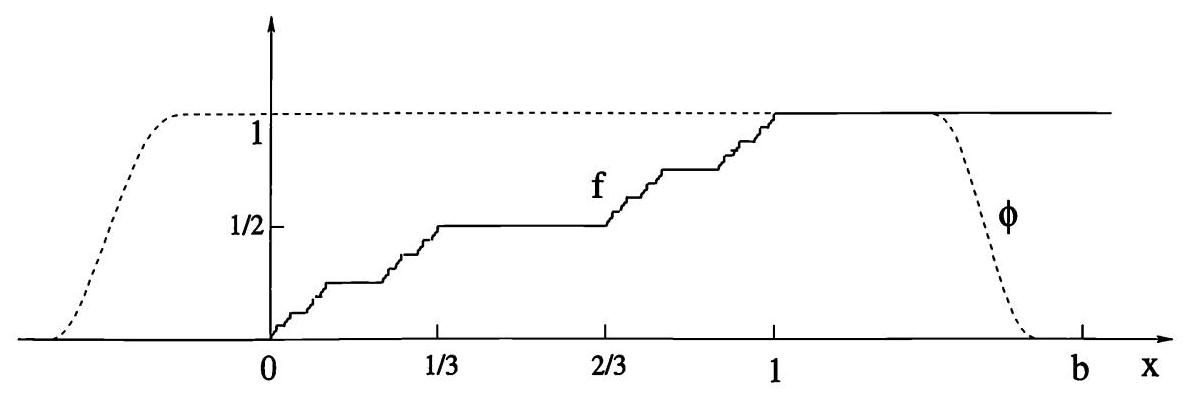
\includegraphics[width=0.9\textwidth]{images/bo_d6ik6nn7aajc739ct1l0_154_150_227_1183_394_0.jpg}
\caption{Cantor函数 $f$ 及一个检验函数 $\phi$ ，表明 $g\left( x\right)  \equiv  0$ 不可能是 $f$ 的弱导数.}
\label{fig:cantor-function-test}
\end{figure}
\noindent 上为常数，故 $g\left( x\right)  = {f}^{\prime }\left( x\right)  = 0$ 必在这些开区间的并集上为零.因此对几乎处处的 $x \in  \mathbb{R}$ ，有 $g\left( x\right)  = 0$ .为导出矛盾，需证明函数 $g \equiv  0$ 并非 $f$ 的弱导数.如图\ref{fig:cantor-function-test}所示，取检验函数 $\phi  \in  {\mathcal{C}}_{c}^{\infty }$ ，使得当 $x \in  \left(  {0,1}\right)$ 时 $\phi \left( x\right)  = 1$ ，而当 $x \geq  b$ 时 $\phi \left( x\right)  = 0$ .则
\[
\int g\left( x\right) \phi \left( x\right) {\d x} = 0 \neq  1 =  - \int f\left( x\right) {\phi }^{\prime }\left( x\right) {\d x}.
\]
\end{instance}

\subsection{分布}
前一节所述构造可推广至多维空间中任意开区域.设 $\Omega  \subseteq  {\mathbb{R}}^{n}$ 为一开集.记 ${L}_{\text{ loc }}^{1}\left( \Omega \right)$ 为 $\Omega$ 上局部可积函数的空间.这些是可测函数 $f : \Omega  \mapsto  \mathbb{R}$ ，其在每个紧子集 $K \subset  \Omega$ 上的限制均可积.

\begin{instance}\label{ins:L1loc-examples}
函数 ${e}^{x}$ 与 $\ln \left| x\right|$ 属于 ${L}_{\text{ loc }}^{1}\left( \mathbb{R}\right)$ ，而 ${x}^{-1} \notin \; {L}_{\text{ loc }}^{1}\left( \mathbb{R}\right)$ .另一方面，函数 $f\left( x\right)  = {x}^{\gamma }$ 对任意(正或负)指数 $\gamma  \in  \mathbb{R}$ 均属于 ${L}_{\text{ loc }}^{1}\left(  \right)  0,\infty \left(  \right)$ .在多个空间维数下，若 $\gamma  < n$ ，则函数 $f\left( x\right)  = {\left| x\right| }^{-\gamma }$ 属于 ${L}_{\text{ loc }}^{1}\left( {\mathbb{R}}^{n}\right)$ .需谨记:函数 $f \in  {L}_{\text{ loc }}^{1}$ 在零测集上的逐点取值无关紧要.
\end{instance}

我们用 ${\mathcal{C}}_{\mathrm{c}}^{\infty }\left( \Omega \right)$ 表示所有阶连续偏导数均存在且连续、支集为 $\Omega$ 的紧子集的连续函数 $\phi  : \Omega  \mapsto  \mathbb{R}$ 所构成的空间.函数 $\phi  \in  {\mathcal{C}}_{\mathrm{c}}^{\infty }\left( \Omega \right)$ 通常称为“检验函数”.我们回顾:函数 $\phi$ 的支集是 $\phi$ 不为零之处的集合的闭包:
\[
\operatorname{Supp}\left( \phi \right)  \doteq  \overline{\{ x \in  \Omega ;\phi \left( x\right)  \neq  0\} }.
\]

我们需要一种高效方式来表示函数 $f$ 的高阶导数.多重指标 $\alpha  = \left( {{\alpha }_{1},{\alpha }_{2},\ldots ,{\alpha }_{n}}\right)$ 是一个由非负整数构成的 $n$ 元组.其长度定义为
\[
\left| \alpha \right|  \doteq  {\alpha }_{1} + {\alpha }_{2} + \cdots  + {\alpha }_{n}.
\]

每个多重指标 $\alpha$ 确定一个阶数为 $\left| \alpha \right|$ 的偏微分算子，即
\[
{D}^{\alpha }f = {\left( \frac{\partial }{\partial {x}_{1}}\right) }^{{\alpha }_{1}}{\left( \frac{\partial }{\partial {x}_{2}}\right) }^{{\alpha }_{2}}\cdots {\left( \frac{\partial }{\partial {x}_{n}}\right) }^{{\alpha }_{n}}f.
\]

\begin{definition}[分布]\label{def:distribution}
开集 $\Omega  \subseteq  {\mathbb{R}}^{n}$ 上的\colorbf{分布}是一个线性泛函 $\Lambda  : {\mathcal{C}}_{c}^{\infty }\left( \Omega \right)  \mapsto  \mathbb{R}$ ，满足如下有界性条件:对每个紧集 $K \subset  \Omega$ ，存在整数 $N \geq  0$ 和常数 $C$ ，使得
\begin{equation}\tag{8.7}\label{eq:distribution-bound}
\left| {\Lambda \left( \phi \right) }\right| \; \leq  \;C\| \phi {\| }_{{\mathcal{C}}^{N}},\;\forall\,\phi  \in  {\mathcal{C}}^{\infty }\,\text{满足}\,\mathrm{{Supp}}\left( \phi \right)  \subseteq  K\;.
\end{equation}
\end{definition}

换言之，对所有在给定紧集 $K$ 外消失的检验函数 $\phi$ ，其值 $\Lambda \left( \phi \right)$ 应以 $\phi$ 的各阶导数(至某阶 $N$ 为止)的最大值为界.

注意，此处 $N$ 与 $C$ 均依赖于紧子集 $K$ .若存在一个与 $K$ 无关的整数 $N \geq  0$ ，使得\eqref{eq:distribution-bound}式成立(其中 $C = \; {C}_{K}$ 仍可依赖于 $K$ )，则称该分布具有有限阶.满足此条件的最小整数 $N$ 称为该分布的阶.

\begin{instance}\label{ins:Lf-is-distribution}
设 $\Omega$ 为 ${\mathbb{R}}^{n}$ 的一个开子集，并考虑函数 $f \in  {L}_{\mathrm{{loc}}c}^{1}\left( \Omega \right)$ .则由下式定义的线性映射 ${\Lambda }_{f} : {\mathcal{C}}_{c}^{\infty }\left( \Omega \right)  \mapsto  \mathbb{R}$
\begin{equation}\tag{8.8}\label{eq:Lf-definition}
{\Lambda }_{f}\left( \phi \right)  \doteq  {\int }_{\Omega }{f\phi \d x}
\end{equation}
是一种分布.事实上，显然 ${\Lambda }_{f}$ 是良定义的且是线性的.对任意紧子集 $K \subset  \Omega$ ，每个支集满足 $\operatorname{Supp}\left( \phi \right)  \subseteq  K$ 的检验函数 $\phi$ 均满足如下估计
\[
\left| {{\Lambda }_{f}\left( \phi \right) }\right| \; = \;\left| {{\int }_{K}f\;\phi \;{\d x}}\right| \; \leq  \;{\int }_{K}\left| {f\left( x\right) }\right| \;{\d x} \cdot  \mathop{\max }\limits_{{x \in  K}}\left| {\phi \left( x\right) }\right| \; \leq  \;C\;\| \phi {\| }_{{\mathcal{C}}^{0}}\;.
\]

因此，界\eqref{eq:distribution-bound}在 $C = {\int }_{K}\left| f\right| {\d x}$ 和 $N = 0$ 下成立.这给出了一个零阶分布的例子.
\end{instance}

所有定义在 $\Omega$ 上的分布构成的族显然构成一个向量空间.一个值得注意的事实是:尽管函数 $f$ 可能(在经典意义下)不存在任何偏导数，但对于任一分布 $\Lambda$ ，总可适当地定义其导数.

\begin{definition}[分布的导数]\label{def:distribution-derivative}
给定一分布 $\Lambda$ 及一多重指标 $\alpha$ ，我们通过下式定义分布 ${D}^{\alpha }\Lambda$
\begin{equation}\tag{8.9}\label{eq:distribution-derivative}
{D}^{\alpha }\Lambda \left( \phi \right)  \doteq  {\left( -1\right) }^{\left| \alpha \right| }\Lambda \left( {{D}^{\alpha }\phi }\right) .
\end{equation}
\end{definition}

易验证 ${D}^{\alpha }\Lambda$ 本身亦为一分布.事实上，映射 $\phi  \mapsto  {D}^{\alpha }\Lambda \left( \phi \right)$ 的线性性是显然的.其次，设 $K$ 是 $\Omega$ 的一个紧子集，且设 $\phi$ 是支集包含于 $K$ 的检验函数.由假设，存在常数 $C$ 和整数 $N \geq  0$ ，使得\eqref{eq:distribution-bound}成立.由此可得
\[
\left| {{D}^{\alpha }\Lambda \left( \phi \right) }\right|  = \left| {\Lambda \left( {{D}^{\alpha }\phi }\right) }\right|  \leq  C{\norm{D}^{\alpha }\phi }_{{\mathcal{C}}^{N}} \leq  C\| \phi {\| }_{{\mathcal{C}}^{N + \left| \alpha \right| }}.
\]

故 ${D}^{\alpha }\Lambda$ 亦满足\eqref{eq:distribution-bound}，其中 $N$ 被替换为 $N + \left| \alpha \right|$ .

注意，若 ${\Lambda }_{f}$ 是\eqref{eq:Lf-definition}中对应于函数 $f$ 的分布，且该函数 $f$ 是 $\left| \alpha \right|$ 次连续可微的，则可通过分部积分得到
{\setjot[-2]\begin{align*}
    {D}^{\alpha }{\Lambda }_{f}\left( \phi \right)  &= {\left( -1\right) }^{\left| \alpha \right| }{\Lambda }_{f}\left( {{D}^{\alpha }\phi }\right)  = {\left( -1\right) }^{\left| \alpha \right| }\int f\left( x\right) {D}^{\alpha }\phi \left( x\right) {\d x}\\
    &= \int {D}^{\alpha }f\left( x\right) \phi \left( x\right) {\d x} = {\Lambda }_{{D}^{\alpha }f}\left( \phi \right) .
\end{align*}}
这证明了公式\eqref{eq:distribution-derivative}的合理性.

\subsection{弱导数}
对每个局部可积函数 $f$ 及每个多重指标 $\alpha  = \left( {{\alpha }_{1},\ldots ,{\alpha }_{n}}\right)$ ，分布 ${\Lambda }_{f}$ 总存在按\eqref{eq:distribution-derivative}定义的分布意义下的导数 ${D}^{\alpha }{\Lambda }_{f}$ .在某些情形下，可找到一个局部可积函数 $g$ ，使得分布 ${D}^{\alpha }{\Lambda }_{f}$ 恰好等于由 ${\Lambda }_{g}$ 所确定的分布.这便引出了弱导数的概念.

\begin{definition}[弱导数]\label{def:weak-derivative}
设 $f \in  {L}_{\text{ loc }}^{1}\left( \Omega \right)$ 是开集 $\Omega  \subseteq  {\mathbb{R}}^{n}$ 上的局部可积函数， ${\Lambda }_{f}$ 是其对应的分布(如\eqref{eq:Lf-definition}所定义).给定一多重指标 $\alpha  = \left( {{\alpha }_{1},\ldots ,{\alpha }_{n}}\right)$ ，若存在局部可积函数 $g \in  {L}_{\text{ loc }}^{1}\left( \Omega \right)$ ，使得 ${D}^{\alpha }{\Lambda }_{f} = {\Lambda }_{g}$ ，即
\begin{equation}\tag{8.10}\label{eq:weak-derivative}
\int f{D}^{\alpha }{\phi \d x} = {\left( -1\right) }^{\left| \alpha \right| }\int {g\phi \d x},\;\forall\,\text{测试函数}\,\phi  \in  {\mathcal{C}}_{\mathrm{c}}^{\infty }\left( \Omega \right) ,
\end{equation}
则称 $g$ 是 $f$ 的\colorbf{弱 $\alpha$ 阶导数}，并记作 $g = {D}^{\alpha }f$ .
\end{definition}

一般而言，弱导数未必存在.特别地，例\ref{ins:heaviside-dirac}表明，Heaviside 函数不具有弱导数.事实上，其分布意义下的导数是一个 Dirac 测度(在原点处集中单位质量)，而非局部可积函数.另一方面，若弱导数存在，则它在几乎处处意义下是唯一的.

\begin{lemma}[弱导数的唯一性]\label{lem:weak-derivative-uniqueness}
设 $f \in  {L}_{\text{ loc }}^{1}\left( \Omega \right)$ ，且 $g,\widetilde{g} \in  {L}_{\text{ loc }}^{1}\left( \Omega \right)$ 是 $f$ 的弱 $\alpha$ 阶导数，即
\[
\int f{D}^{\alpha }{\phi \d x} = {\left( -1\right) }^{\left| \alpha \right| }\int {g\phi \d x} = {\left( -1\right) }^{\left| \alpha \right| }\int \widetilde{g}{\phi \d x}
\]
对所有检验函数 $\phi  \in  {\mathcal{C}}_{\mathrm{c}}^{\infty }\left( \Omega \right)$ 成立.则 $g\left( x\right)  = \widetilde{g}\left( x\right)$ 几乎处处成立于 $x \in  \Omega$ .
\end{lemma}

\begin{proof}
由假设，函数 $\left( {g - \widetilde{g}}\right)  \in  {L}_{\text{ loc }}^{1}\left( \Omega \right)$ 满足
\[
\int \left( {g - \widetilde{g}}\right) {\phi \d x} = 0,\;\forall\,\text{测试函数}\,\phi  \in  {\mathcal{C}}_{\mathrm{c}}^{\infty }\left( \Omega \right) .
\]

因此，由附录中推论A.17可得 $g\left( x\right)  - \widetilde{g}\left( x\right)  = 0$几乎处处成立于 $x \in  \Omega$ .
\end{proof}

若函数 $f$ 二阶连续可微，则微积分基本定理指出:偏导数可交换顺序，即 ${f}_{{x}_{j}{x}_{k}} = {f}_{{x}_{k}{x}_{j}}$ .该性质对弱导数仍成立.为一般性地陈述此结果，我们回顾:两个多重指标 $\alpha  = \left( {{\alpha }_{1},\ldots ,{\alpha }_{n}}\right)$ 与 $\beta  = \left( {{\beta }_{1},\ldots ,{\beta }_{n}}\right)$ 的和定义为 $\alpha  + \beta  = \left( {{\alpha }_{1} + {\beta }_{1},\ldots ,{\alpha }_{n} + {\beta }_{n}}\right)$ .

\begin{lemma}[弱导数可交换]\label{lem:weak-derivative-commute}
设 $f \in  {L}_{\text{ loc }}^{1}\left( \Omega \right)$ 对每个 $\left| \alpha \right|  \leq  k$ 均存在弱导数 ${D}^{\alpha }f$ .则对任意满足 $\left| \alpha \right|  + \left| \beta \right|  \leq  k$ 的多重指标对 $\alpha ,\beta$ ，有
\begin{equation}\tag{8.11}\label{eq:weak-derivative-commute}
{D}^{\alpha }\left( {{D}^{\beta }f}\right)  = {D}^{\beta }\left( {{D}^{\alpha }f}\right)  = {D}^{\alpha  + \beta }f.
\end{equation}
\end{lemma}

\begin{proof}
考虑任意检验函数 $\phi  \in  {\mathcal{C}}_{c}^{\infty }\left( \Omega \right)$ .利用 ${D}^{\beta }\phi  \in \; {\mathcal{C}}_{\mathrm{c}}^{\infty }\left( \Omega \right)$ 同样是检验函数，可得
{\setjot[-2]\begin{align*}
    {\int }_{\Omega }{D}^{\alpha }f{D}^{\beta }{\phi \d x} &= {\left( -1\right) }^{\left| \alpha \right| }{\int }_{\Omega }f\left( {{D}^{\alpha  + \beta }\phi }\right) {\d x}\\
    &= {\left( -1\right) }^{\left| \alpha \right| }{\left( -1\right) }^{\left| \alpha  + \beta \right| }{\int }_{\Omega }\left( {{D}^{\alpha  + \beta }f}\right) {\phi \d x}\\
    &= {\left( -1\right) }^{\left| \beta \right| }{\int }_{\Omega }\left( {{D}^{\alpha  + \beta }f}\right) {\phi \d x}.
\end{align*}}



由定义，这意味着 ${D}^{\alpha  + \beta }f = {D}^{\beta }\left( {{D}^{\alpha }f}\right)$ .在前述计算中交换多重指标 $\alpha$ 与 $\beta$ 的角色，可得 ${D}^{\alpha  + \beta }f = \; {D}^{\alpha }\left( {{D}^{\beta }f}\right)$ .
\end{proof}

下一个引理推广了另一熟知结论:极限的弱导数等于弱导数的极限.

\begin{lemma}[弱导数的收敛性]\label{lem:weak-derivative-convergence}
考虑函数列 ${f}_{n} \in  {L}_{\text{ loc }}^{1}\left( \Omega \right)$ .对固定多重指标 $\alpha$ ，假设每个 ${f}_{n}$ 均存在弱导数 ${g}_{n} = {D}^{\alpha }{f}_{n}$ .若 ${f}_{n} \rightarrow  f$ 且 ${g}_{n} \rightarrow  g$ 在 ${L}_{\text{ loc }}^{1}\left( \Omega \right)$ 中成立，则 $g = {D}^{\alpha }f$ .
\end{lemma}

\begin{proof}
对任一检验函数 $\phi  \in  {\mathcal{C}}_{\mathrm{c}}^{\infty }\left( \Omega \right)$ ，直接计算可得
{\begin{align*}
    {\int }_{\Omega }{g\phi \d x} &= \mathop{\lim }\limits_{{n \rightarrow  \infty }}{\int }_{\Omega }{g}_{n}{\phi \d x} = \mathop{\lim }\limits_{{n \rightarrow  \infty }}{\left( -1\right) }^{\left| \alpha \right| }{\int }_{\Omega }{f}_{n}{D}^{\alpha }{\phi \d x}\\
    &= {\left( -1\right) }^{\left| \alpha \right| }{\int }_{\Omega }f{D}^{\alpha }{\phi \d x}
\end{align*}}
根据定义，这意味着 $g$ 是 $f$ 的 $\alpha$ 阶弱导数.
\end{proof}

\section{磨光化}

如常，设 $\Omega  \subseteq  {\mathbb{R}}^{n}$ 为开集.对给定的 $\varepsilon  > 0$ ，定义开子集
\begin{equation}\tag{8.12}\label{eq:omega-epsilon}
{\Omega }_{\varepsilon } \doteq  \left\{  {x \in  {\mathbb{R}}^{n};\bar{B}\left( {x,\varepsilon }\right)  \subset  \Omega }\right\}  .
\end{equation}

对每个 $u \in  {L}_{\text{ loc }}^{1}\left( \Omega \right)$ ，磨光化
\[
{u}_{\varepsilon }\left( x\right)  \doteq  \left( {{J}_{\varepsilon } * u}\right) \left( x\right)  = {\int }_{B\left( {x,\varepsilon }\right) }{J}_{\varepsilon }\left( {x - y}\right) u\left( y\right) {\d y}
\]
对每个 $x \in  {\Omega }_{\varepsilon }$ 均有定义.此外， ${u}_{\varepsilon } \in  {\mathcal{C}}^{\infty }\left( {\Omega }_{\varepsilon }\right)$ .磨光化算子一个极为有用的性质是:它与弱微分可交换.

\begin{lemma}[磨光化与弱导数可交换]\label{lem:mollification}
设 ${\Omega }_{\varepsilon } \subset  \Omega$ 如式\eqref{eq:omega-epsilon}所定义.假设函数 $u \in  {L}_{\text{ loc }}^{1}\left( \Omega \right)$ 存在弱导数 ${D}^{\alpha }u$ ，其中 $\alpha$ 为某多重指标.则其磨光化的导数(在经典意义下存在)恰等于该弱导数的磨光化，即
\begin{equation}\tag{8.13}\label{eq:mollification-derivative}
{D}^{\alpha }\left( {{J}_{\varepsilon } * u}\right)  = {J}_{\varepsilon } * {D}^{\alpha }u,\;\forall\,x \in  {\Omega }_{\varepsilon }.
\end{equation}
\end{lemma}

\begin{proof}
    对每个固定的 $x \in  {\Omega }_{\varepsilon }$ ，函数 $\phi \left( y\right)  \doteq  {J}_{\varepsilon }\left( {x - y}\right)\in{\mathcal{C}}_{c}^{\infty }\left( \Omega \right)$ .因此可将弱导数定义 ${D}^{\alpha }u$ 应用于检验函数 $\phi$ .记 ${D}_{x}^{\alpha }$ 与 ${D}_{y}^{\alpha }$ 分别表示关于变量 $x$ 或 $y$ 的微分，从而得到
{\setjot[-2]\begin{align*}
    {D}^{\alpha }{u}_{\varepsilon }\left( x\right) &= {D}_{x}^{\alpha }\left( {{\int }_{\Omega }{J}_{\varepsilon }\left( {x - y}\right) u\left( y\right) {\d y}}\right)\\
    &= {\int }_{\Omega }{D}_{x}^{\alpha }{J}_{\varepsilon }\left( {x - y}\right) u\left( y\right) {\d y}\\
    &= {\left( -1\right) }^{\left| \alpha \right| }{\int }_{\Omega }{D}_{y}^{\alpha }{J}_{\varepsilon }\left( {x - y}\right) u\left( y\right) {\d y}\\
    &= {\left( -1\right) }^{\left| \alpha \right|  + \left| \alpha \right| }{\int }_{\Omega }{J}_{\varepsilon }\left( {x - y}\right) {D}_{y}^{\alpha }u\left( y\right) {\d y}\\
    &= \left( {{J}_{\varepsilon } * {D}^{\alpha }u}\right) \left( x\right) .
\end{align*}}
\end{proof}

\begin{figure}[htbp]
    \vspace{-0.5 em}
\centering
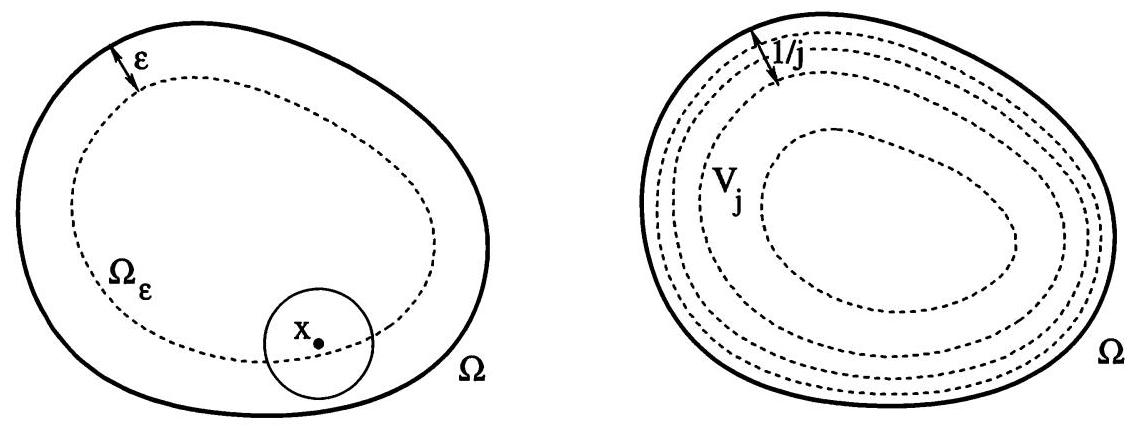
\includegraphics[width=0.85\textwidth]{images/bo_d6ik6nn7aajc739ct1l0_159_171_1175_1136_426_0.jpg}
\caption{左:到边界距离$> \varepsilon$ 的点构成的开子集 ${\Omega }_{\varepsilon } \subset  \Omega$ ；右:区域 $\Omega$ 可被可数个开子域 ${V}_{j} = {\Omega }_{1/\left( {j - 1}\right) } \setminus  {\overline{\Omega }}_{1/\left( {j + 1}\right) }$ 覆盖.}
\label{fig:omega-epsilon}
\end{figure}

引理\ref{lem:mollification}中所述磨光化的这一性质，为关联弱导数与经典意义下的偏导数提供了关键工具.作为首个应用，我们证明

\begin{corollary}[常值函数]\label{cor:constant-function}
设 $\Omega  \subseteq  {\mathbb{R}}^{n}$ 为连通开集，且假设 $u \in  {L}_{\text{ loc }}^{1}\left( \Omega \right)$ .若 $u$ 的一阶弱导数满足
\[
{D}_{{x}_{i}}u\left( x\right)  = 0,\;i = 1,2,\ldots ,n,\,\text{ a.e. }x \in  \Omega ,
\]

则 $u$ 几乎处处等于一常值函数.
\end{corollary}

\begin{proof}
1. 对 $\varepsilon  > 0$ ，考虑其磨光化函数 ${u}_{\varepsilon } = {J}_{\varepsilon } * u$ .由前述分析， ${u}_{\varepsilon } : {\Omega }_{\varepsilon } \mapsto  \mathbb{R}$ 是光滑函数，其导数 ${D}_{{x}_{i}}{u}_{\varepsilon }$ 在 ${\Omega }_{\varepsilon }$ 上恒为零.因此， ${u}_{\varepsilon }$ 在 ${\Omega }_{\varepsilon }$ 的每个连通分支上必为常数.

\noindent 2. 现考虑任意两点 $x,y \in  \Omega$ .由于开集 $\Omega$ 是连通的，故存在一条折线路径 $\Gamma$ ，连接 $x$ 与 $y$ ，且完全位于 $\Omega$ 内部.令 $\delta  \doteq  \mathop{\min }\limits_{{z \in  \Gamma }}d\left( {z,\partial \Omega }\right)  > 0$ 为 $\Gamma$ 中各点到 $\Omega$ 边界的最小距离.则对每个 $\varepsilon  < \delta$ ，整条折线 $\Gamma$ 均位于 ${\Omega }_{\varepsilon }$ 内.因此， $x,y$ 属于 ${\Omega }_{\varepsilon }$ 的同一连通分支.特别地， ${u}_{\varepsilon }\left( x\right)  = {u}_{\varepsilon }\left( y\right) .$ 

\noindent 3. 设 $\widetilde{u}\left( x\right)  \doteq  \mathop{\lim }\limits_{{\varepsilon  \rightarrow  0}}{u}_{\varepsilon }\left( x\right)$ .由前一步可知， $\widetilde{u}$ 在 $\Omega$ 上为常函数.此外， $\widetilde{u}\left( x\right)  = u\left( x\right)$ 在 $u$ 的每个Lebesgue点处成立，故在 $\Omega$ 上几乎处处成立.
\end{proof}

\begin{figure}[htbp]
\centering
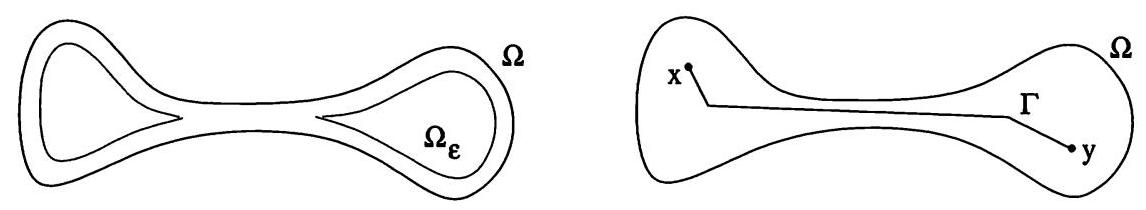
\includegraphics[width=0.9\textwidth]{images/bo_d6ik6nn7aajc739ct1l0_160_166_1087_1146_210_0.jpg}
\caption{左:即使 $\Omega$ 连通，子区域 ${\Omega }_{\varepsilon } \doteq \; \{ x \in  \Omega ;\bar{B}\left( {x,\varepsilon }\right)  \subseteq  \Omega \}$ 也可能不连通.右:任意两点 $x,y \in  \Omega$ 均可通过一条完全位于 $\Omega$ 内部的折线路径 $\Gamma$ 相连.因此，若 $\varepsilon  > 0$ 足够小，则 $x$ 与 $y$ 属于 ${\Omega }_{\varepsilon }$ 的同一连通分支.}
\label{fig:omega-epsilon-components}
\end{figure}

在一维情形下，再次借助引理\ref{lem:mollification}，我们现刻画具有 ${L}^{1}$ 中弱导数的函数集合.

\begin{corollary}[绝对连续函数]\label{cor:absolute-continuity}
设 $(a,b)$ 为一开区间，并设 $u \in  {L}_{\text{ loc }}^{1}\left(a,b\right)$ 具有弱导数 $v \in \; {L}^{1}\left( {( a,b) }\right)$ .则存在一个绝对连续函数 $\widetilde{u}$ ，使得
\begin{equation}\tag{8.14}\label{eq:ac-representative}
\widetilde{u}\left( x\right)  = u\left( x\right) \;\text{a.e. }x \in  ( a,b) ,
\end{equation}
\begin{equation}\tag{8.15}\label{eq:ac-classical-derivative}
v\left( x\right)  = \mathop{\lim }\limits_{{h \rightarrow  0}}\frac{\widetilde{u}\left( {x + h}\right)  - \widetilde{u}\left( x\right) }{h}\;\text{a.e. }x \in  ( a,b) .
\end{equation}
\end{corollary}

\begin{proof}
设 ${x}_{0} \in  ( a,b)$ 为 $u$ 的一个Lebesgue点，并定义
\[
\widetilde{u}\left( x\right)  \doteq  u\left( {x}_{0}\right)  + {\int }_{{x}_{0}}^{x}v\left( y\right) {\d y}.
\]

显然， $\widetilde{u}$ 绝对连续且满足\eqref{eq:ac-classical-derivative}.

为证\eqref{eq:ac-representative}，设 ${J}_{\varepsilon }$ 为标准磨光核，并令 ${u}_{\varepsilon } \doteq \; {J}_{\varepsilon } * u,{v}_{\varepsilon } \doteq  {J}_{\varepsilon } * v$ .则 ${u}_{\varepsilon },{v}_{\varepsilon } \in  {\mathcal{C}}^{\infty }\left( {( a + \varepsilon ,b - \varepsilon ) }\right)$ ，而引理\ref{lem:mollification}给出
\begin{equation}\tag{8.16}\label{eq:ac-mollified-fundamental}
{u}_{\varepsilon }\left( x\right)  = {u}_{\varepsilon }\left( {x}_{0}\right)  + {\int }_{{x}_{0}}^{x}{v}_{\varepsilon }\left( y\right) {\d y}\;\forall\,x \in  ( a + \varepsilon ,b - \varepsilon ) .
\end{equation}

令 $\varepsilon  \rightarrow  0$ ，我们得到 ${u}_{\varepsilon }\left( {x}_{0}\right)  \rightarrow  u\left( {x}_{0}\right)$ ，因为 ${x}_{0}$ 是一个Lebesgue点.此外，\eqref{eq:ac-mollified-fundamental}式右端对每个 $x \in  ( a,b)$ 均收敛于 $\widetilde{u}\left( x\right)$ ，而左端在 $u$ 的每个Lebesgue点(从而几乎处处)收敛于 $u\left( x\right)$ .因此\eqref{eq:ac-representative}成立.
\end{proof}
\begin{property}[弱可微函数]
若 $f,g \in  {L}_{\text{ loc }}^{1}\left( \Omega \right)$ 是弱可微函数，则对任意常数 $a,b \in  \mathbb{R}$ ，其线性组合 ${af} + {bg}$ 也弱可微，且满足
\begin{equation}\tag{8.17}\label{eq:weak-derivative-linearity}
{D}_{{x}_{i}}\left( {{af} + {bg}}\right)  = a{D}_{{x}_{i}}f + b{D}_{{x}_{i}}g.
\end{equation}
\end{property}



我们现在考虑弱可微函数的乘积与复合.需注意，一般地，两个函数 $f,g \in  {L}_{\text{ loc }}^{1}$ 的乘积未必是局部可求和的；类似地，定义在 ${\mathbb{R}}^{n}$ 上的两个弱可微函数的乘积也未必弱可微(参见习题 20).因此，在下一引理中，我们将假设其中一函数连续可微且其导数一致有界.

给定两个多重指标 $\alpha  = \left( {{\alpha }_{1},\ldots ,{\alpha }_{n}}\right)$ 和 $\beta  = \left( {{\beta }_{1},\ldots ,{\beta }_{n}}\right)$ ，我们回顾记号 $\beta  \leq  \alpha$ 表示对每个 $i = 1,\ldots ,n$ 均有 ${\beta }_{i} \leq  {\alpha }_{i}$ .此外，
\[
\begin{pmatrix}\alpha\\ \beta \end{pmatrix}\begin{pmatrix}\alpha\\ \beta \end{pmatrix}  \doteq  \frac{\alpha !}{\beta !\left( {\alpha  - \beta }\right) !} \doteq  \frac{{\alpha }_{1}!}{{\beta }_{1}!\left( {{\alpha }_{1} - {\beta }_{1}}\right) !} \cdot  \frac{{\alpha }_{2}!}{{\beta }_{2}!\left( {{\alpha }_{2} - {\beta }_{2}}\right) !}\cdots \frac{{\alpha }_{n}!}{{\beta }_{n}!\left( {{\alpha }_{n} - {\beta }_{n}}\right) !}.
\]
    
\begin{lemma}[弱可微函数的乘积与复合]\label{lem:weakly-differentiable-product-composition}
设 $\Omega  \subseteq  {\mathbb{R}}^{n}$ 为任意开集，并考虑函数 $u \in  {L}_{\text{ loc }}^{1}\left( \Omega \right)$ ，其具有任意阶 $\left| \alpha \right|  \leq  k$ 的弱导数 ${D}^{\alpha }u$ .
\begin{enumerate}[(i)]
    \item 若 $\eta  \in  {\mathcal{C}}^{k}\left( \Omega \right)$ ，则乘积 ${\eta u}$ 存在阶数不超过 $k$ 的弱导数.这些弱导数由莱布尼茨公式给出
\begin{equation}\tag{8.18}\label{eq:weak-leibniz}
{D}^{\alpha }\left( {\eta u}\right)  = \sum_{{\beta  \leq  \alpha }}\begin{pmatrix}\alpha\\ \beta \end{pmatrix} {D}^{\beta }\eta {D}^{\alpha  - \beta }u.
\end{equation}
    \item 设 ${\Omega }^{\prime } \subseteq  {\mathbb{R}}^{n}$ 为一开集， $\varphi  : {\Omega }^{\prime } \mapsto  \Omega$ 为一 ${\mathcal{C}}^{k}$ 双射，其雅可比矩阵具有一致有界逆.则复合函数 $u \circ  \varphi$ 属于 ${L}_{\text{ loc }}^{1}\left( {\Omega }^{\prime }\right)$ ，且存在阶数不超过 $k$ 的弱导数.
\end{enumerate}
\end{lemma}

\begin{proof}
1. 为证 (i)，令 ${J}_{\varepsilon }$ 为标准磨光子，并设 ${u}_{\varepsilon } \doteq  {J}_{\varepsilon } * u$ .由于莱布尼茨公式对光滑函数之乘积成立，故对每个 $\varepsilon  > 0$ ，我们得到
\begin{equation}\tag{8.19}\label{eq:weak-leibniz-mollified}
{D}^{\alpha }\left( {\eta {u}_{\varepsilon }}\right)  = \sum_{{\beta  \leq  \alpha }}\begin{pmatrix}\alpha\\ \beta \end{pmatrix} {D}^{\beta }\eta {D}^{\alpha  - \beta }{u}_{\varepsilon }.
\end{equation}

于是，对任一检验函数 $\phi  \in  {\mathcal{C}}_{c}^{\infty }\left( \Omega \right)$ ，有
{\begin{align*}
    {\left( -1\right) }^{\left| \alpha \right| }{\int }_{\Omega }\left( {\eta {u}_{\varepsilon }}\right) {D}^{\alpha }{\phi \d x} &= {\int }_{\Omega }{D}^{\alpha }\left( {\eta {u}_{\varepsilon }}\right) {\phi \d x} \\
    &= \sum_{{\beta  \leq  \alpha }}\begin{pmatrix}\alpha\\ \beta \end{pmatrix} {\int }_{\Omega }\left( {{D}^{\beta }\eta {D}^{\alpha  - \beta }{u}_{\varepsilon }}\right) {\phi \d x}.
\end{align*}}


注意:若 $\varepsilon  > 0$ 足够小，使得 $\operatorname{Supp}\left( \phi \right)  \subset  {\Omega }_{\varepsilon }$ ，则上述积分定义良好.令 $\varepsilon  \rightarrow  0$ ，可得
\[
{\left( -1\right) }^{\left| \alpha \right| }{\int }_{\Omega }\left( {\eta u}\right) {D}^{\alpha }{\phi \d x} = {\int }_{\Omega }\left( {\sum_{{\beta  \leq  \alpha }}\begin{pmatrix}\alpha\\ \beta \end{pmatrix} {D}^{\beta }\eta {D}^{\alpha  - \beta }u}\right) {\phi \d x}.
\]

由弱导数定义，式\eqref{eq:weak-leibniz}成立.

\noindent 2. 我们对 $k$ 归纳证明 (ii).记 $y$ 为 ${\Omega }^{\prime }$ 中的变量， $x = \varphi \left( y\right)$ 为 $\Omega$ 中的变量，如图\ref{fig:composition-map}所示.由假设， $n \times  n$ 雅可比矩阵 ${\left( \frac{\partial {\varphi }_{i}}{\partial {y}_{j}}\right) }_{i,j = 1,\ldots ,n}$ 具有一致有界逆.因此复合函数 $u \circ  \varphi$ 属于 ${L}_{\text{ loc }}^{1}\left( {\Omega }^{\prime }\right)$ ，从而定理在 $k = 0$ 情形下得证.

接下来，假设结论对所有阶数为 $\left| \alpha \right|  \leq \; k - 1$ 的弱导数均成立.取任一检验函数 $\phi  \in  {\mathcal{C}}_{c}^{\infty }\left( {\Omega }^{\prime }\right)$ ，并定义其磨光 ${u}_{\varepsilon } \doteq  {J}_{\varepsilon } * u$ .对任意足够小的 $\varepsilon  > 0$ 使得 $\varphi \left( {\operatorname{Supp}\left( \phi \right) }\right)  \subset  {\Omega }_{\varepsilon }$，有
{\begin{align*}
    - {\int }_{{\Omega }^{\prime }}\left( {{u}_{\varepsilon } \circ  \varphi }\right)  \cdot  {D}_{{y}_{i}}{\phi \d y} &= {\int }_{{\Omega }^{\prime }}{D}_{{y}_{i}}\left( {{u}_{\varepsilon } \circ  \varphi }\right)  \cdot  {\phi \d y}\\
    &= {\int }_{{\Omega }^{\prime }}\left( {\sum_{{j = 1}}^{n}{D}_{{x}_{j}}{u}_{\varepsilon }\left( {\varphi \left( y\right) }\right)  \cdot  {D}_{{y}_{i}}{\varphi }_{j}\left( y\right) }\right)  \cdot  \phi \left( y\right) {\d y}.
\end{align*}}

令 $\varepsilon  \rightarrow  0$ ，我们得出复合函数 $u \circ  \varphi$ 存在一阶弱导数，其表达式为
\begin{equation}\tag{8.20}\label{eq:weak-chain-rule}
{D}_{{y}_{i}}\left( {u \circ  \varphi }\right) \left( y\right)  = \sum_{{j = 1}}^{n}{D}_{{x}_{j}}u\left( {\varphi \left( y\right) }\right)  \cdot  {D}_{{y}_{i}}{\varphi }_{j}\left( y\right) .
\end{equation}

根据归纳假设，每个函数 ${D}_{{x}_{j}}\left( {u \circ  \varphi }\right)$ 均存在阶数不超过 $k - 1$ 的弱导数，而 ${D}_{{y}_{i}}{\varphi }_{j} \in  {\mathcal{C}}^{k - 1}\left( {\Omega }^{\prime }\right)$ .由引理第 (i) 部分可知，式\eqref{eq:weak-chain-rule}右端所有乘积均存在阶数不超过 $k - 1$ 的弱导数.再应用引理\ref{lem:weak-derivative-commute}，可得复合函数 $u \circ  \varphi$ 存在阶数不超过 $k$ 的弱导数.由此通过归纳法，证毕.
\end{proof}

\begin{figure}[htbp]
\centering
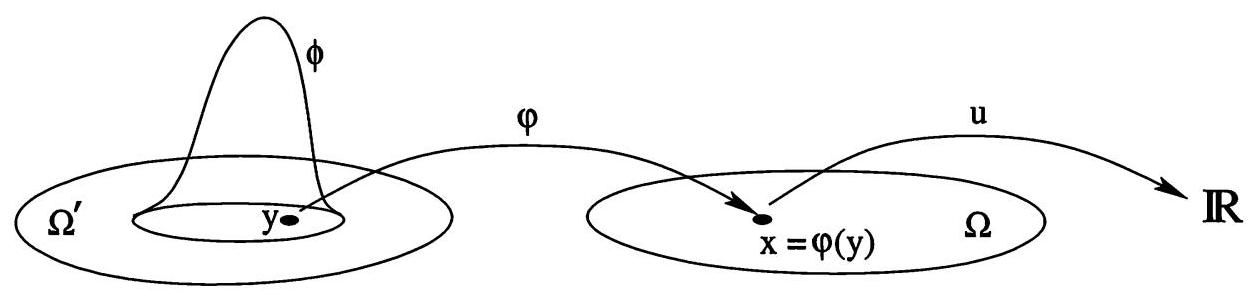
\includegraphics[width=1.0\textwidth]{images/bo_d6ik6nn7aajc739ct1l0_163_113_942_1254_295_0.jpg}
\caption{引理\ref{lem:weakly-differentiable-product-composition} 第 (ii) 部分所考虑的映射.}
\label{fig:composition-map}
\end{figure}

\section{Soblev空间}

考虑开集 $\Omega  \subseteq  {\mathbb{R}}^{n}$ ，固定 $p \in  \left(  {1,\infty }\right)$ ，并设 $k$ 为一非负整数.

\begin{definition}[Soblev空间]\label{def:sobolev-space}
(i) Soblev空间 ${W}^{k,p}\left( \Omega \right)$ 是指所有局部可积函数 $u : \Omega  \mapsto  \mathbb{R}$ 构成的空间，使得对每个满足 $\left| \alpha \right|  \leq  k$ 的多重指标 $\alpha$ ，其弱导数 ${D}^{\alpha }u$ 存在且属于 ${L}^{p}\left( \Omega \right)$ .

在 ${W}^{k,p}$ 上，我们采用如下范数:
\begin{equation}\tag{8.21}\label{eq:sobolev-norm-p}
\| u{\| }_{{W}^{k,p}} \doteq  {\left( \sum_{{\left| \alpha \right|  \leq  k}}{\int }_{\Omega }{\left| {D}^{\alpha }u\right| }^{p}\d x\right) }^{1/p},\;1 \leq  p < \infty ,
\end{equation}
\begin{equation}\tag{8.22}\label{eq:sobolev-norm-infty}
\| u{\| }_{{W}^{k,\infty }} \doteq  \sum_{{\left| \alpha \right|  \leq  k}}\underset{x \in  \Omega }{\operatorname{ess}\sup }\left| {{D}^{\alpha }u}\right|,\;p = \infty .
\end{equation}

(ii) 子空间 ${W}_{0}^{k,p}\left( \Omega \right)  \subseteq  {W}^{k,p}\left( \Omega \right)$ 定义为 ${\mathcal{C}}_{c}^{\infty }\left( \Omega \right)$ 在 ${W}^{k,p}\left( \Omega \right)$ 中的闭包.更准确地说， $u \in  {W}_{0}^{k,p}\left( \Omega \right)$ 当且仅当存在一列函数 ${u}_{n} \in  {\mathcal{C}}_{c}^{\infty }\left( \Omega \right)$ ，使得
\[
{\norm{u - u_n}}_{{W}^{k,p}} \rightarrow  0.
\]

(iii) 此外， ${W}_{\text{ loc }}^{k,p}\left( \Omega \right)$ 表示所有局部属于 ${W}^{k,p}$ 的函数构成的空间.这些函数 $u : \Omega  \mapsto  \mathbb{R}$ 满足如下性质:若开集 ${\Omega }^{\prime } \subset  \subset  \Omega$\footnotemark，则 $u$ 在 ${\Omega }^{\prime }$ 上的限制属于 ${W}^{k,p}\left( {\Omega }^{\prime }\right)$ .
\end{definition}
\footnotetext{根据定义，集合 ${\Omega }^{\prime }$ 紧包含于 $\Omega$ ，是指其闭包 $\overline{{\Omega }^{\prime }}$ 是 $\Omega$ 的一个紧子集.}

直观上，可将闭子空间 ${W}_{0}^{1,p}\left( \Omega \right)$ 视为所有在 $\Omega$ 边界上消失的函数 $u \in  {W}^{1,p}\left( \Omega \right)$ 构成的空间.更一般地， ${W}_{0}^{k,p}\left( \Omega \right)$ 是一类函数空间，其导数 ${D}^{\alpha }u$ 在 $\partial \Omega$ 上消失，其中 $\left| \alpha \right|  \leq  k - 1$ .

\begin{definition}[Hilbert-Soblev空间]\label{def:hilbert-sobolev-space}
在$p = 2$ 下，定义\colorbf{Hilbert-Soblev 空间}${H}^{k}\left( \Omega \right)  \doteq  {W}^{k,2}\left( \Omega \right)$，并赋予如下内积:
\begin{equation}\tag{8.23}\label{eq:hilbert-sobolev-inner-product}
\langle u,v{\rangle }_{{H}^{k}} \doteq  \sum_{{\left| \alpha \right|  \leq  k}}{\int }_{\Omega }{D}^{\alpha }u{D}^{\alpha }{v\d x}.
\end{equation}

类似地，定义 ${H}_{0}^{k}\left( \Omega \right)  \doteq  {W}_{0}^{k,2}\left( \Omega \right)$ .
\end{definition}

\begin{theorem}[Soblev空间的基本性质]\label{thm:sobolev-basic-properties}
(i) 每个 Soblev 空间 ${W}^{k,p}\left( \Omega \right)$ 都是一个 Banach 空间.

(ii) 空间 ${W}_{0}^{k,p}\left( \Omega \right)$ 是 ${W}^{k,p}\left( \Omega \right)$ 的一个闭子空间，因此它是一个 Banach 空间，且范数与 ${W}^{k,p}\left( \Omega \right)$ 相同.

(iii) 空间 ${H}^{k}\left( \Omega \right)$ 和 ${H}_{0}^{k}\left( \Omega \right)$ 均为 Hilbert 空间.
\end{theorem}

\begin{proof}
1. 设 $u,v \in  {W}^{k,p}\left( \Omega \right)$ .对 $\left| \alpha \right|  \leq  k$ ，称 ${D}^{\alpha }u,{D}^{\alpha }v$ 为其弱导数.则对任意 $\lambda ,\mu  \in  \mathbb{R}$，线性组合 ${\lambda u} + {\mu v}$ 是一个局部可和函数.易验证其弱导数为
\begin{equation}\tag{8.24}\label{eq:sobolev-weak-derivative-linearity}
{D}^{\alpha }\left( {{\lambda u} + {\mu v}}\right)  = \lambda {D}^{\alpha }u + \mu {D}^{\alpha }v.
\end{equation}
因此，对每个 $\left| \alpha \right|  \leq  k$ ，有 ${D}^{\alpha }\left( {{\lambda u} + {\mu v}}\right)  \in  {L}^{p}\left( \Omega \right)$ .这表明 ${W}^{k,p}\left( \Omega \right)$ 是一个向量空间.


\noindent 2. 接下来验证式\eqref{eq:sobolev-norm-p}与式\eqref{eq:sobolev-norm-infty}满足定义范数的条件 (N1)-(N3).对 $\lambda  \in  \mathbb{R}$ 和 $u \in  {W}^{k,p}$ ，有
\begin{gather*}
    \| {\lambda u}{\| }_{{W}^{k,p}} = \left| \lambda \right| \| u{\| }_{{W}^{k,p}}\\
    \| u{\| }_{{W}^{k,p}} \geq  \| u{\| }_{{L}^{p}} \geq  0
\end{gather*}
且等号成立当且仅当 $u = 0$ .

此外，若 $u,v \in  {W}^{k,p}\left( \Omega \right)$ ，则对 $1 \leq  p < \infty$ ，Minkowski不等式给出
{\begin{align*}
    \| u + v{\| }_{{W}^{k,p}} &= {\left( \sum_{{\left| \alpha \right|  \leq  k}}{\norm{{D}^{\alpha }u + {D}^{\alpha }v}_{{L}^{p}}^{p}}\right) }^{1/p}\\
    &\leq  {\left( \sum_{{\left| \alpha \right|  \leq  k}}{\left( {\norm{D^{\alpha }u}}_{{L}^{p}} + {\norm{D^{\alpha }v}}_{{L}^{p}}\right) }^{p}\right) }^{1/p}\\
    &\leq  {\left( \sum_{{\left| \alpha \right|  \leq  k}}{\norm{D^{\alpha }u}_{{L}^{p}}^{p}}\right) }^{1/p} + {\left( \sum_{{\left| \alpha \right|  \leq  k}}{\norm{D^{\alpha }v}_{{L}^{p}}^{p}}\right) }^{1/p}\\
    &= \| u{\| }_{{W}^{k,p}} + \| v{\| }_{{W}^{k,p}}.
\end{align*}}

在 $p = \infty$ 的情形下，上述计算替换为
{\begin{align*}
    \| u + v{\| }_{{W}^{k,\infty }} &= \sum_{{\left| \alpha \right|  \leq  k}}{\norm{D^{\alpha }u + {D}^{\alpha }v}}_{{L}^{\infty }} \leq  \sum_{{\left| \alpha \right|  \leq  k}}\left( {{\norm{D^{\alpha }u}}_{{L}^{\infty }} + {\norm{D^{\alpha }v}}_{{L}^{\infty }}}\right)\\
    &= \| u{\| }_{{W}^{k,\infty }} + \| v{\| }_{{W}^{k,\infty }}.
\end{align*}}


\noindent 3. 为完成 (i) 的证明，需证空间 ${W}^{k,p}\left( \Omega \right)$ 是完备的，故为 Banach 空间.

设 ${\left( {u}_{n}\right) }_{n \geq  1}$ 是 ${W}^{k,p}\left( \Omega \right)$ 中的一个 Cauchy 序列.对任一满足 $\left| \alpha \right|  \leq  k$ 的多重指标 $\alpha$ ，弱导数序列 ${D}^{\alpha }{u}_{n}$ 在 ${L}^{p}\left( \Omega \right)$ 中为 Cauchy 序列.由于 ${L}^{p}\left( \Omega \right)$ 完备，故存在函数 $u$ 和 ${u}_{\alpha }$ ，使得
\begin{equation}\tag{8.25}\label{eq:sobolev-cauchy-convergence}
\| {u}_{n} - u{\| }_{{L}^{p}} \rightarrow  0,\;\| {D}^{\alpha }{u}_{n} - {u}_{\alpha }{\| }_{{L}^{p}} \rightarrow  0\;\forall\,\left| \alpha \right|  \leq  k.
\end{equation}

由引理\ref{lem:weak-derivative-convergence}，极限函数 ${u}_{\alpha }$ 恰为弱导数 ${D}^{\alpha }u$ .因该结论对所有满足 $\left| \alpha \right|  \leq  k$ 的多重指标 $\alpha$ 成立，故收敛 ${u}_{n} \rightarrow \; u$ 在 ${W}^{k,p}\left( \Omega \right)$ 中成立.至此，(i) 得证.

\noindent 4. ${W}_{0}^{k,p}\left( \Omega \right)$ 是 ${W}^{k,p}\left( \Omega \right)$ 的闭子空间这一事实直接由定义得出.同样易验证式\eqref{eq:hilbert-sobolev-inner-product}是一个内积，其所诱导的范数为 $\|  \cdot  {\| }_{{W}^{k,2}}$ .
\end{proof}

\begin{instance}\label{ins:W1p-interval-ac}
设 $\Omega = (a,b)$ 为一开区间.由推论\ref{cor:absolute-continuity}可知，空间 ${W}^{1,p}\left( {( a,b) }\right)$ 的每个元素几乎处处等于某个绝对连续函数 $f : (a,b) \mapsto  \mathbb{R}$ ，且该函数的导数为 ${f}^{\prime } \in  {L}^{p}\left( {( a,b) }\right)$ .\par
\begin{figure}[htbp]
\centering
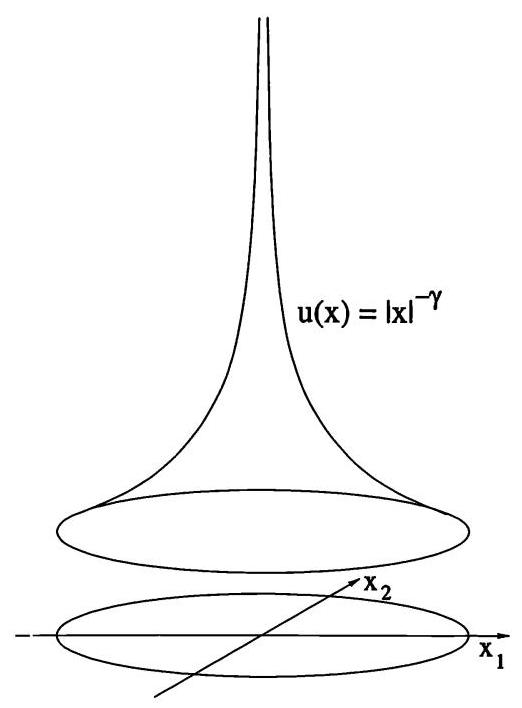
\includegraphics[width=0.35\textwidth]{images/bo_d6ik6nn7aajc739ct1l0_166_479_682_522_708_0.jpg}
\caption{对某些 $p,n$ 取值，函数 $u \in  {W}^{1,p}\left( {\mathbb{R}}^{n}\right)$ 可能不连续或无界.}
\label{fig:W1p-discontinuous}
\end{figure}
\end{instance}



\begin{instance}\label{ins:radial-singularity-W1p}
设 $\Omega  = B\left( {0,1}\right)  \subset  {\mathbb{R}}^{n}$ 为以原点为中心、半径为一的开球.固定 $\gamma  > 0$ ，并考虑径向对称函数
\[
u\left( x\right)  \doteq  {\left| x\right| }^{-\gamma } = {\left( \sum_{{i = 1}}^{n}{x}_{i}^{2}\right) }^{-\gamma /2},\;0 < \left| x\right|  < 1.
\]

注意到 $u \in  {\mathcal{C}}^{1}\left( {\Omega \setminus \{ 0\} }\right)$ .我们声称:对 $1 \leq  p < \infty$ ，
\begin{equation}\tag{8.26}\label{eq:radial-W1p-condition}
u \in  {W}^{1,p}\left( \Omega \right)\iff \gamma  < \frac{n - p}{p}.
\end{equation}

在原点之外，偏导数计算如下:
\begin{equation}\tag{8.27}\label{eq:radial-W1p-derivative}
{u}_{{x}_{i}} =  - \frac{\gamma }{2}{\left( \sum_{{i = 1}}^{n}{x}_{i}^{2}\right) }^{-\left( {\gamma /2}\right)  - 1}2{x}_{i} = \frac{-\gamma {x}_{i}}{{\left| x\right| }^{\gamma  + 2}}.
\end{equation}

因此，梯度 $\nabla u = \left( {{u}_{{x}_{1}},\ldots ,{u}_{{x}_{n}}}\right)$ 的欧氏范数为
\[
\left| {\nabla u\left( x\right) }\right|  = {\left( \sum_{{i = 1}}^{n}{\left| {u}_{{x}_{i}}\left( x\right) \right| }^{2}\right) }^{1/2} = \frac{\gamma }{{\left| x\right| }^{\gamma  + 1}}.
\]

记 ${\sigma }_{n}$ 为单位球面 $\{ x \in  {\mathbb{R}}^{n};\left| x\right|  = 1\}$ 的 $\left( {n - 1}\right)$ 维测度，我们计算得
\begin{equation}\tag{8.28}\label{eq:radial-W1p-integral}
    \setjot[-2]\begin{aligned}
        {\int }_{\Omega }{\left( \frac{1}{{\left| x\right| }^{\gamma  + 1}}\right) }^{p}{\d x} &= {\int }_{x \in  {\mathbb{R}}^{n},\left| x\right|  < 1}{\left| x\right| }^{-p\left( {\gamma  + 1}\right) }{\d x}\\
        &= {\sigma }_{n}{\int }_{0}^{1}{r}^{n - 1}{r}^{-p\left( {\gamma  + 1}\right) }{\d r}.
    \end{aligned}
\end{equation}

式\eqref{eq:radial-W1p-integral}右端有限当且仅当 $n - 1 - p\left( {\gamma  + 1}\right)  >  - 1$ ，即 $\gamma  < \frac{n - p}{p}$ .对 ${\left| u\right| }^{p}$ 作类似计算后，我们得出
\[
{\int }_{\Omega }\left( {{\left| u\right| }^{p} + {\left| \nabla u\right| }^{p}}\right) {\d x} < \infty \iff \gamma  < \frac{n - p}{p}.
\]

为完成式\eqref{eq:radial-W1p-condition}的证明，需验证:若 $0 < \gamma  < \frac{n - p}{p}$ (从而 $n \geq  2$ )，则式\eqref{eq:radial-W1p-derivative}中所定义的函数确为 $u$ 在整个球 $\Omega$ 上的弱导数(而不仅限于集合 $\Omega  \setminus  \{ 0\}$ 上).为此，取任意检验函数 $\phi  \in  {\mathcal{C}}_{c}^{\infty }\left( \Omega \right)$ .固定 $i \in  \{ 1,\ldots ,n\}$ .为方便起见，我们将 $\phi$ 延拓至整个空间 ${\mathbb{R}}^{n}$ ，即令 $\phi \left( x\right)  = 0$ 对所有 $x \notin  \Omega$ 成立.由于 $n \geq  2$ ， ${x}_{i}$ 轴的 $n$ 维 Lebesgue 测度为零.分部积分得
{\setjot[-2]\begin{align*}
    {\int }_{\Omega }\frac{-\gamma {x}_{i}}{{\left| x\right| }^{\gamma  + 2}}{\phi \d x} &= {\int }_{{\mathbb{R}}^{n - 1}\setminus \{ 0\} }\left( {{\int }_{\mathbb{R}}\frac{-\gamma {x}_{i}}{{\left| x\right| }^{\gamma  + 2}}\phi {\d x_{i}}}\right) \d x_{1}\cdots \d x_{i - 1}\d x_{i + 1}\cdots \d x_{n}\\
    &=  - {\int }_{{\mathbb{R}}^{n - 1}\setminus \{ 0\} }\left( {{\int }_{\mathbb{R}}{\left| x\right| }^{-\gamma }{\phi }_{{x}_{i}}\d x_{i}}\right) \d x_{1}\cdots \d x_{i - 1}\d x_{i + 1}\cdots \d x_{n}\\
    &=  - {\int }_{\Omega }{\left| x\right| }^{-\gamma }{\phi }_{{x}_{i}}{\d x}.
\end{align*}}


注意，前述计算依赖于 $u$ 在几乎每条平行于某坐标轴的直线上绝对连续(事实上光滑)这一事实.然而，无法通过在零测集上修改 $u$ ，使其在整个区域 $\Omega$ 上连续.
\end{instance}

Soblev空间中其一重要问题是:能否用函数一阶导数的范数来估计该函数的范数？ \par
以下结果为此提供了初等估计.它对包含于某一层状区域(例如) $\Omega$ 的区域成立.
\begin{equation}\tag{8.29}\label{eq:poincare-strip-domain}
\Omega  \subseteq  \left\{  {x = \left( {{x}_{1},{x}_{2},\ldots ,{x}_{n}}\right) ;a < {x}_{1} < b}\right\}  .
\end{equation}

\begin{theorem}[Poincaré不等式，I]\label{thm:poincare-inequality-I}
设 $\Omega  \subset  {\mathbb{R}}^{n}$ 是满足式\eqref{eq:poincare-strip-domain}的某个 $a,b \in  \mathbb{R}$ 的开集.则每个 $u \in  {H}_{0}^{1}\left( \Omega \right)$ 均满足
\begin{equation}\tag{8.30}\label{eq:poincare-inequality-I}
\| u{\| }_{{L}^{2}\left( \Omega \right) }\; \leq  \;2\left( {b - a}\right) \;\| {D}_{{x}_{1}}u{\| }_{{L}^{2}\left( \Omega \right) }.
\end{equation}
\end{theorem}

\begin{proof}
1. 首先假设 $u \in  {\mathcal{C}}_{c}^{\infty }\left( \Omega \right)$ .我们将 $u$ 延拓至全空间 ${\mathbb{R}}^{n}$ ，定义为对 $x \notin  \Omega$ 取 $u\left( x\right)  = 0$ .引入变量 $x = \left( {{x}_{1},{x}^{\prime }}\right)$ ，其中 ${x}^{\prime } = \left( {{x}_{2},\ldots ,{x}_{n}}\right)$ ，计算得
\[
{u}^{2}\left( {{x}_{1},{x}^{\prime }}\right)  = {\int }_{a}^{{x}_{1}}{2u}{u}_{{x}_{1}}\left( {t,{x}^{\prime }}\right) {\d t}.
\]

分部积分得
{\setjot[-2]\begin{align*}
    \| u{\| }_{{L}^{2}}^{2} &= {\int }_{{\mathbb{R}}^{n}}{u}^{2}\left( x\right) {\d x} = {\int }_{{\mathbb{R}}^{n - 1}}{\int }_{a}^{b}1 \cdot  \left( {{\int }_{a}^{{x}_{1}}{2u}{u}_{{x}_{1}}\left( {t,{x}^{\prime }}\right) {\d t}}\right) \d x_{1}\d x^{\prime }\\
    &= {\int }_{{\mathbb{R}}^{n - 1}}{\int }_{a}^{b}\left( {b - {x}_{1}}\right) {2u}{u}_{{x}_{1}}\left( {{x}_{1},{x}^{\prime }}\right) \d x_{1}\d x^{\prime } \leq  2\left( {b - a}\right) {\int }_{{\mathbb{R}}^{n}}\left| u\right| \left| {u}_{{x}_{1}}\right| {\d x}\\
    &\leq  2\left( {b - a}\right) \| u{\| }_{{L}^{2}}{\norm{u}_{{x}_{1}}}_{{L}^{2}}
\end{align*}}


两边同除以 $\| u{\| }_{{L}^{2}}$ ，即得对每个 $u \in  {\mathcal{C}}_{c}^{\infty }\left( \Omega \right)$ 成立的式\eqref{eq:poincare-inequality-I}.

\noindent 2. 现考虑任意 $u \in  {H}_{0}^{1}\left( \Omega \right)$ .由假设，存在函数列 ${u}_{n} \in  {\mathcal{C}}_{c}^{\infty }\left( \Omega \right)$，使得 ${\norm{u}_{n} - u}_{{H}^{1}} \rightarrow  0$.由前一步可知
\[
\| u{\| }_{{L}^{2}} = \mathop{\lim }\limits_{{n \rightarrow  \infty }}{\norm{u}_{n}}_{{L}^{2}} \leq  \mathop{\lim }\limits_{{n \rightarrow  \infty }}2\left( {b - a}\right) {\norm{D_{{x}_{1}}{u}_{n}}}_{{L}^{2}} = 2\left( {b - a}\right) {\norm{D_{{x}_{1}}u}}_{{L}^{2}}.\qedhere
\]
\end{proof}

为继续分析Soblev空间，我们需要建立关于弱导数的一些额外事实.

\begin{theorem}[弱导数的性质]\label{thm:weak-derivative-properties}
设 $\Omega  \subseteq  {\mathbb{R}}^{n}$ 为开集， $p \in  \left(  {1,\infty }\right)$ ，且 $\left| \alpha \right|  \leq  k$ .若 $u,v \in  {W}^{k,p}\left( \Omega \right)$ ，则:
\begin{enumerate}
    \item $u$ 在任意开集 $\widetilde{\Omega } \subset  \Omega$ 上的限制属于空间 ${W}^{k,p}\left( \widetilde{\Omega }\right)$ .
    \item ${D}^{\alpha }u \in  {W}^{k - \left| \alpha \right| ,p}\left( \Omega \right)$ .
    \item 若 $\eta  \in  {\mathcal{C}}^{k}\left( \Omega \right)$ ，则乘积满足 ${\eta u} \in  {W}^{k,p}\left( \Omega \right)$ .此外，存在仅依赖于 $\Omega$ 和 $\| \eta {\| }_{{\mathcal{C}}^{k}}$，但不依赖于 $u,$ 的常数 $C$ ，使得
\begin{equation}\tag{8.31}\label{eq:eta-u-Wkp-estimate}
\norm{\eta u}_{{W}^{k,p}\left( \Omega \right) } \leq C\norm{u}_{{W}^{k,p}\left( \Omega \right) }.
\end{equation}
    \item 设 ${\Omega }^{\prime } \subseteq  {\mathbb{R}}^{n}$ 为开集， $\varphi  : {\Omega }^{\prime } \mapsto  \Omega$ 为 ${\mathcal{C}}^{k}$ 微分同胚，其Jacobi矩阵的逆一致有界.则复合函数满足 $u \circ  \varphi  \in  {W}^{k,p}\left( {\Omega }^{\prime }\right)$ .此外，存在仅依赖于 ${\Omega }^{\prime }$ 和 $\| \varphi {\| }_{{\mathcal{C}}^{k}}$ 、但不依赖于 $u$ 的常数 $C$ ，使得
\begin{equation}\tag{8.32}\label{eq:composition-Wkp-estimate}
\norm{u \circ  \varphi }_{{W}^{k,p}\left( {\Omega }^{\prime }\right) }\leq  C\norm{u}_{{W}^{k,p}\left( \Omega \right) }.
\end{equation}
\end{enumerate}
\end{theorem}

\begin{proof}
命题 (i) 是定义的直接推论，而 (ii) 由引理\ref{lem:weak-derivative-commute}得出.

为证 (iii)，我们注意到:由假设， $\eta$ 的所有导数均有界，即
\[
{\norm{D^{\beta }\eta }}_{{L}^{\infty }} \leq  \| \eta {\| }_{{\mathcal{C}}^{k}},\;\forall\,\left| \beta \right|  \leq  k.
\]

因此，由表示公式\eqref{eq:weak-leibniz}即得估计式\eqref{eq:eta-u-Wkp-estimate}.

回顾引理\ref{lem:weakly-differentiable-product-composition}的第(ii)部分，我们对 $k$ 作归纳法证明 (iv).由假设， $n \times  n$ 雅可比矩阵 ${\left( {D}_{{x}_{i}}{\varphi }_{j}\right) }_{i,j = 1,\ldots ,n}$ 具有一致有界逆.因此 $k = 0$ 的情形显然成立.

接下来，假设结论对 $k = 0,1,\ldots ,m - 1$ 成立.若 $u \in \; {W}^{m,p}\left( \Omega \right)$ ，则有
\[
\| {D}_{{x}_{i}}\left( {u \circ  \varphi }\right) {\| }_{{W}^{m - 1,p}\left( {\Omega }^{\prime }\right) }\; \leq  \;{C}^{\prime }\;\| \nabla u{\| }_{{W}^{m - 1,p}\left( \Omega \right) }\| \varphi {\| }_{{\mathcal{C}}^{m}\left( {\Omega }^{\prime }\right) }\; \leq  \;C\;\| u{\| }_{{W}^{m,p}\left( \Omega \right) }.
\]

表明结论对 $k = m$ 亦成立.由归纳法，结论成立.
\end{proof}

\section{Soblev函数的逼近}

若 $u \in  {W}^{k,p}\left( {\mathbb{R}}^{n}\right)$ 是定义在整个空间 ${\mathbb{R}}^{n}$ 上的函数，则可通过取磨光来简单地用光滑函数逼近: ${u}_{\varepsilon } = \; {J}_{\varepsilon } * u$ .然而，若 $u$ 仅定义在某个开子集 $\Omega  \subset  {\mathbb{R}}^{n}$ 上，则需更精细的构造.

\begin{theorem}[用光滑函数逼近]\label{thm:approximation-by-smooth-functions}
设 $\Omega  \subseteq  {\mathbb{R}}^{n}$ 为开集， $u \in  {W}^{k,p}\left( \Omega \right)$ 满足 $1 \leq  p < \infty$ .则对任意 $\varepsilon  > 0$ ，存在函数 $U \in  {\mathcal{C}}^{\infty }\left( \Omega \right)$ 使得 $\| U - u{\| }_{{W}^{k,p}\left( \Omega \right) } < \varepsilon$ .
\end{theorem}

\begin{proof}
1. 给定 $\varepsilon  > 0$ .考虑集合 $\Omega$ 的如下局部有限开覆盖(见图\ref{fig:omega-epsilon}):
\begin{gather*}
{V}_{1} \doteq  \left\{  {x \in  \Omega ;d\left( {x,\partial \Omega }\right)  > \frac{1}{2}}\right\}\\
{V}_{j} \doteq  \left\{  {x \in  \Omega ;\frac{1}{j + 1} < d\left( {x,\partial \Omega }\right)  < \frac{1}{j - 1}}\right\}  ,\;j = 2,3,\ldots
\end{gather*}

利用附录中定理A.18，令 ${\eta }_{1},{\eta }_{2},\ldots$ 为从属于上述覆盖的光滑单位分解.由定理\ref{thm:weak-derivative-properties}，对每个 $j \geq  0$ ，乘积 ${\eta }_{j}u$ 属于 ${W}^{k,p}\left( \Omega \right)$ .依构造，其支集包含于 ${V}_{j}$ .

\noindent 2. 考虑磨光 ${J}_{\varepsilon } * \left( {{\eta }_{j}u}\right)$ .由引理\ref{lem:mollification}及附录中定理A.16，对每个 $\left| \alpha \right|  \leq  k$ ，有
\[
{D}^{\alpha }\left( {{J}_{\varepsilon } * \left( {{\eta }_{j}u}\right) }\right)  = {J}_{\epsilon } * \left( {{D}^{\alpha }\left( {{\eta }_{j}u}\right) }\right)  \rightarrow  {D}^{\alpha }\left( {{\eta }_{j}u}\right),\varepsilon\to 0
\]

由于每个 ${\eta }_{j}$ 具有紧支集，此处收敛在 ${L}^{p}\left( \Omega \right)$ 中发生.因此，对每个 $j \geq  0$ ，可取 $0 < {\varepsilon }_{j} < {2}^{-j}$ 足够小使得
\[
{\norm{\eta _{j}u - {J}_{{\varepsilon }_{j}} * \left( {\eta }_{j}u\right) }}_{{W}^{k,p}\left( \Omega \right) } \leq  \varepsilon {2}^{-j}.
\]

\noindent 3. 考虑函数
\[
U \doteq  \sum_{{j = 1}}^{\infty }{J}_{{\varepsilon }_{j}} * \left( {{\eta }_{j}u}\right)
\]

注意，上述级数在 ${W}^{k,p}$ 中未必收敛.但其必逐点收敛，因为任一紧集 $K \subset  \Omega$ 仅与有限个集合 ${V}_{j}$ 相交.限制在 $K$ 上时，上述和式仅含有限个非零项.由于每项均光滑，故有 $U \in \; {\mathcal{C}}^{\infty }\left( \Omega \right)$ .

\noindent 4. 考虑子区域
\[
{\Omega }_{1/n} \doteq  \left\{  {x \in  \Omega ;d\left( {x,\partial \Omega }\right)  > \frac{1}{n}}\right\}  .
\]

由 $\sum_{j}{\eta }_{j}\left( x\right)  \equiv  1$ 可知，对每个 $n \geq  1$ ，得到
\[
\| U - u{\| }_{{W}^{k,p}\left( {\Omega }_{1/n}\right) } \leq  \sum_{{j = 1}}^{{n + 2}}{\norm{\eta _{j}u - {J}_{{\varepsilon }_{j}} * \left( {\eta }_{j}u\right) }}_{{W}^{k,p}\left( {\Omega }_{1/n}\right) } \leq  \sum_{{j = 1}}^{{n + 2}}\varepsilon {2}^{-j} \leq  \varepsilon .
\]

由此推出
\[
\norm{U - u}_{{W}^{k,p}\left( \Omega \right) } = \mathop{\sup }\limits_{{n \geq  1}}\norm{U - u}_{{W}^{k,p}\left( {\Omega }_{1/n}\right) } \leq  \varepsilon .
\]

由于 $\varepsilon  > 0$ 是任意的，这证明了 ${\mathcal{C}}^{\infty }$ 函数集在 ${W}^{k,p}\left( \Omega \right)$ 中稠密.
\end{proof}

利用上述逼近结果，我们得到Soblev函数的第一个正则性定理(见图\ref{fig:omega-cylinder-domain}).

\begin{theorem}[弱导数与强导数之间的关系]\label{thm:weak-strong-derivative}
设 $u \in  {W}^{1,1}\left( \Omega \right)$ ，其中 $\Omega  \subseteq  {\mathbb{R}}^{n}$ 为具有如下形式的开集\eqref{eq:omega-cylinder-domain}
\begin{equation}\tag{8.33}\label{eq:omega-cylinder-domain}
\Omega  = \left\{  {x = \left( {x,{x}^{\prime }}\right) ;{x}^{\prime } \doteq  \left( {{x}_{2},\ldots ,{x}_{n}}\right)  \in  {\Omega }^{\prime },\alpha \left( {x}^{\prime }\right)  < {x}_{1} < \beta \left( {x}^{\prime }\right) }\right\}
\end{equation}

(可能取 $\alpha  \equiv   - \infty$ 或 $\beta  \equiv   + \infty$ ).则存在函数 $\widetilde{u}$ ，使得对几乎处处的 $x \in  \Omega$ ，有 $\widetilde{u}\left( x\right)  = u\left( x\right)$ ，且满足以下条件:对几乎处处的 ${x}^{\prime } = \; \left( {{x}_{2},\ldots ,{x}_{n}}\right)  \in  {\Omega }^{\prime } \subset  {\mathbb{R}}^{n - 1}$ (关于 $\left( {n - 1}\right)$ 维Lebesgue测度)，映射
\[
{x}_{1} \mapsto  \widetilde{u}\left( {{x}_{1},{x}^{\prime }}\right)
\]

是绝对连续的；其导数几乎处处等于弱导数 ${D}_{{x}_{1}}u$ .
\end{theorem}

\begin{figure}[htbp]
\centering
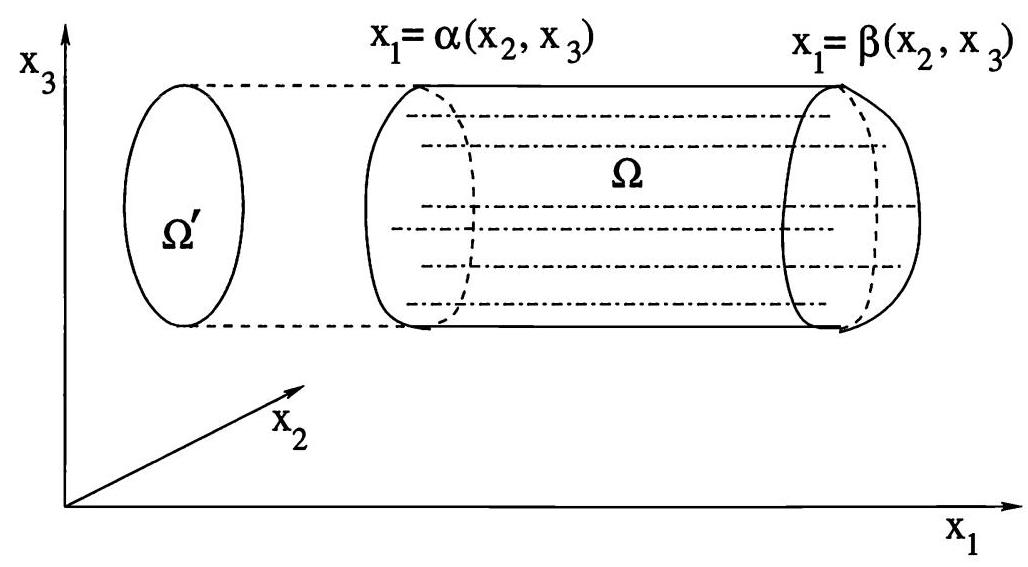
\includegraphics[width=0.9\textwidth]{images/bo_d6ik6nn7aajc739ct1l0_171_221_1182_1028_567_0.jpg}
\caption{\eqref{eq:omega-cylinder-domain}式中的定义域 $\Omega$ .若 $u$ 具有弱导数 ${D}_{{x}_{1}}u \in  {L}^{1}\left( \Omega \right)$ ，则(通过在零测集上修改其取值)函数 $u$ 在几乎每条平行于 ${x}_{1}$ 轴的线段上绝对连续，且其偏导数 $\partial u/\partial {x}_{1}$ 几乎处处等于该弱导数.}
\label{fig:omega-cylinder-domain}
\end{figure}

\begin{proof}
1. 由定理\ref{thm:approximation-by-smooth-functions}，存在一列函数 ${u}_{k} \in  {\mathcal{C}}^{\infty }\left( \Omega \right)$ ，使得
\begin{equation}\tag{8.34}\label{eq:uk-converge-W11}
{\norm{u}_{k} - u}_{{W}^{1,1}} < {2}^{-k}
\end{equation}

我们断言，这蕴含逐点收敛性
\[
{u}_{k}\left( x\right)  \rightarrow  u\left( x\right) ,\;{D}_{{x}_{1}}{u}_{k}\left( x\right)  \rightarrow  {D}_{{x}_{1}}u\left( x\right) \;\text{ for a.e. }x \in  \Omega .
\]

事实上，考虑函数
\begin{equation}\tag{8.35}\label{eq:def-fg-series}
{\setjot[-2]\begin{aligned}
f\left( x\right)  &\doteq  \left| {{u}_{1}\left( x\right) }\right|  + \sum_{{k = 1}}^{\infty }\left| {{u}_{k + 1}\left( x\right)  - {u}_{k}\left( x\right) }\right| \\
g\left( x\right)  &\doteq  \left| {{D}_{{x}_{1}}{u}_{1}\left( x\right) }\right|  + \sum_{{k = 1}}^{\infty }\left| {{D}_{{x}_{1}}{u}_{k + 1}\left( x\right)  - {D}_{{x}_{1}}{u}_{k}\left( x\right) }\right| .
\end{aligned}}
\end{equation}

由\eqref{eq:uk-converge-W11}，
\[
{\norm{u}_{k} - {u}_{k + 1}}_{{W}^{1,1}} \leq  {2}^{1 - k}
\]

因此 $f,g \in  {L}^{1}\left( \Omega \right)$ ，且\eqref{eq:def-fg-series}式中的级数对几乎处处的 $x \in  \Omega$ 绝对收敛，故其几乎处处逐点收敛.此外，我们还有如下估计
\begin{equation}\tag{8.36}\label{eq:uk-bounded-by-fg}
\left| {{u}_{k}\left( x\right) }\right| \leq  f\left( x\right) ,\quad \left| {{D}_{{x}_{1}}{u}_{k}\left( x\right) }\right| \leq  g\left( x\right),\forall\,k \geq  1,\;x \in  \Omega .
\end{equation}

\noindent 2. 由于 $f,g \in  {L}^{1}\left( \Omega \right)$ ，由Fubini定理，存在一个零测集 $\mathcal{N} \subset  {\Omega }^{\prime }$ (关于 $\left( {n - 1}\right)$ 维Lebesgue测度)，使得对每个 ${x}^{\prime } \in  {\Omega }^{\prime } \setminus  \mathcal{N}$ ，均有
\begin{equation}\tag{8.37}\label{eq:fg-integrable-slices}
{\int }_{\alpha \left( {x}^{\prime }\right) }^{\beta \left( {x}^{\prime }\right) }f\left( {{x}_{1},{x}^{\prime }}\right) \d x_{1} < \infty ,\quad {\int }_{\alpha \left( {x}^{\prime }\right) }^{\beta \left( {x}^{\prime }\right) }g\left( {{x}_{1},{x}^{\prime }}\right) \d x_{1} < \infty .
\end{equation}

固定这样一个点 ${x}^{\prime } \in  {\Omega }^{\prime } \setminus  \mathcal{N}$ .选取一点 ${y}_{1} \in  ( \alpha \left( {x}^{\prime }\right) ,\beta \left( {x}^{\prime }\right) )$ ，使得逐点收敛 ${u}_{k}\left( {{y}_{1},{x}^{\prime }}\right)  \rightarrow  u\left( {{y}_{1},{x}^{\prime }}\right)$ 成立.对任意 $\alpha \left( {x}^{\prime }\right)  < {x}_{1} < \; \beta \left( {x}^{\prime }\right)$ ，因 ${u}_{k}$ 光滑，故有
\begin{equation}\tag{8.38}\label{eq:uk-line-integral}
{u}_{k}\left( {{x}_{1},{x}^{\prime }}\right)  = {u}_{k}\left( {{y}_{1},{x}^{\prime }}\right)  + {\int }_{{y}_{1}}^{{x}_{1}}{D}_{{x}_{1}}{u}_{k}\left( {s,{x}^{\prime }}\right) {\d s}.
\end{equation}

现令 $k \rightarrow  \infty$ 趋于\eqref{eq:uk-line-integral}式中右侧极限.由\eqref{eq:uk-bounded-by-fg}与\eqref{eq:fg-integrable-slices}，函数 ${D}_{{x}_{1}}{u}_{k}\left( {\cdot ,{x}^{\prime }}\right)$ 均被可积函数 $g\left( {\cdot ,{x}^{\prime }}\right)  \in  {L}^{1}$ 控制.根据控制收敛定理，\eqref{eq:uk-line-integral}式右侧从而收敛于
\begin{equation}\tag{8.39}\label{eq:def-u-tilde}
\widetilde{u}\left( {{x}_{1},{x}^{\prime }}\right)  \doteq  u\left( {{y}_{1},{x}^{\prime }}\right)  + {\int }_{{y}_{1}}^{{x}_{1}}{D}_{{x}_{1}}u\left( {s,{x}^{\prime }}\right) {\d s}.
\end{equation}

显然，\eqref{eq:def-u-tilde}式右侧是标量变量 ${x}_{1}$ 的绝对连续函数.另一方面，左侧满足
\[
\widetilde{u}\left( {{x}_{1},{x}^{\prime }}\right)  \doteq  \mathop{\lim }\limits_{{n \rightarrow  \infty }}{u}_{k}\left( {{x}_{1},{x}^{\prime }}\right)  = u\left( {{x}_{1},{x}^{\prime }}\right) \;\text{ for a.e. }{x}_{1} \in  \left(  {\alpha \left( {x}^{\prime }\right) ,\beta \left( {x}^{\prime }\right) }\right)  .
\]

至此，证明完成.
\end{proof}

\begin{remark}\label{rem:weak-strong-derivative}
(i) 显然，对任意其他导数 ${D}_{{x}_{i}}u$ (含 $i = 1,2,\ldots ,n$ )，类似结论均成立.

(ii) 若 $u \in  {W}^{k,p}\left( \widetilde{\Omega }\right)$ 且 $\Omega  \subset  \widetilde{\Omega }$ ，则 $u$ 在 $\Omega$ 上的限制属于空间 ${W}^{k,p}\left( \Omega \right)$ .即使开集 $\widetilde{\Omega }$ 具有复杂拓扑结构，定理\ref{thm:weak-strong-derivative}的结论仍可应用于任一具有表示式\eqref{eq:omega-cylinder-domain}的柱状子区域 $\Omega  \subset  \widetilde{\Omega }$ .

(iii) 若 $\Omega  \subset  {\mathbb{R}}^{n}$ 是有界开集且 $u \in  {W}^{k,p}\left( \Omega \right)$ ，则对每个 $q \in  \left(  {1,p}\right)$ 均有 $u \in  {W}^{k,q}\left( \Omega \right)$ .

\end{remark}

\section{延拓算子}

设 $\Omega  \subset  {\mathbb{R}}^{n}$ 为具有 ${\mathcal{C}}^{1}$ 边界的有界开区域\footnote{说 $\Omega$ 具有 ${\mathcal{C}}^{1}$ 边界，是指如下含义:对每个边界点 $x \in  \partial \Omega$ ，均存在 $x$ 的一个邻域 ${V}^{x}$ 及一个 ${\mathcal{C}}^{1}$ 映射 $\varphi  : {\mathbb{R}}^{n} \mapsto  \mathbb{R}$ ，使得 $\nabla \varphi \left( x\right)  \neq  0$ 且 $\Omega  \cap  {V}^{x} = \left\{  {y \in  {V}^{x};\varphi \left( y\right)  > 0}\right\}  .$}.对定义在 $\Omega$ 上的函数 $u$ ，下述定理提供了一种将其延拓至整个空间 ${\mathbb{R}}^{n}$ 的方法，并在 ${W}^{1,p}$ 范数上保持某种控制.

\begin{theorem}[延拓算子]\label{thm:extension-operator}
设 $\Omega  \subset   \subset  \widetilde{\Omega } \subset  {\mathbb{R}}^{n}$ 为开集，且 $\Omega$ 的闭包是 $\widetilde{\Omega }$ 的紧子集.此外，假设 $\Omega$ 具有 ${\mathcal{C}}^{1}$ 边界.则存在有界线性算子 $E$ : ${W}^{1,p}\left( \Omega \right)  \mapsto  {W}^{1,p}\left( {\mathbb{R}}^{n}\right)$ 及常数 $C$ ，使得

(i) ${Eu}\left( x\right)  = u\left( x\right)$ 对几乎处处的 $x \in  \Omega$ 成立，

(ii) $Eu\left( x\right)  = 0$ 对 $x \notin  \widetilde{\Omega }$ 成立，

(iii) 满足估计式 $\| {Eu}{\| }_{{W}^{1,p}\left( {\mathbb{R}}^{n}\right) } \leq  C\| u{\| }_{{W}^{1,p}\left( \Omega \right) }$ .
\end{theorem}

\begin{proof}
1. 我们首先证明:当区域为半空间 $\Omega  = \left\{  {x = \left( {{x}_{1},{x}_{2},\ldots ,{x}_{n}}\right) ;{x}_{1} > 0}\right\}$ 且 $\widetilde{\Omega } = {\mathbb{R}}^{n}$ 时，结论同样成立.此时，任意函数 $u \in  {W}^{1,p}\left( \Omega \right)$ 均可通过对称反射延拓至整个空间 ${\mathbb{R}}^{n}$ ，即定义为
\begin{equation}\tag{8.40}\label{eq:extension-reflection}
\left( {{E}^{\sharp }u}\right) \left( {{x}_{1},{x}_{2},\ldots ,{x}_{n}}\right)  \doteq  u\left( {\left| {x}_{1}\right| ,{x}_{2},{x}_{3},\ldots ,{x}_{n}}\right) .
\end{equation}

由定理\ref{thm:weak-strong-derivative}可知，对每个 $i \in  \{ 1,\ldots ,n\}$ ，函数 $u$ 在几乎每条平行于 ${x}_{i}$ -轴的直线上绝对连续.因此，其延拓 ${E}^{\sharp }u$ 亦然.通过分部积分的直接计算可知， ${E}^{\sharp }u$ 在全空间 ${\mathbb{R}}^{n}$ 上存在一阶弱导数，且满足
\[
\left\{  \begin{array}{ll} {D}_{{x}_{1}}{E}^{\sharp }u\left( {-{x}_{1},{x}_{2},\ldots ,{x}_{n}}\right) &  =  - {D}_{{x}_{1}}u\left( {{x}_{1},{x}_{2},\ldots ,{x}_{n}}\right) , \\  {D}_{{x}_{j}}{E}^{\sharp }u\left( {-{x}_{1},{x}_{2},\ldots ,{x}_{n}}\right) &  = {D}_{{x}_{j}}u\left( {{x}_{1},{x}_{2},\ldots ,{x}_{n}}\right) \;\left( {j = 2,\ldots ,n}\right) , \end{array}\right.
\]

对所有 ${x}_{1} > 0,{x}_{2},\ldots ,{x}_{n} \in  \mathbb{R}$ 成立.在\eqref{eq:extension-reflection}处定义的延拓算子 ${E}^{\sharp } : {W}^{1,p}\left( \Omega \right)  \mapsto \; {W}^{1,p}\left( {\mathbb{R}}^{n}\right)$ 显然是线性的，且是有界的，因为
\[
\| {E}^{\sharp }u{\| }_{{W}^{1,p}\left( {\mathbb{R}}^{n}\right) } \leq  2\| u{\| }_{{W}^{1,p}\left( \Omega \right) }.
\]




\begin{figure}[htbp]
\centering
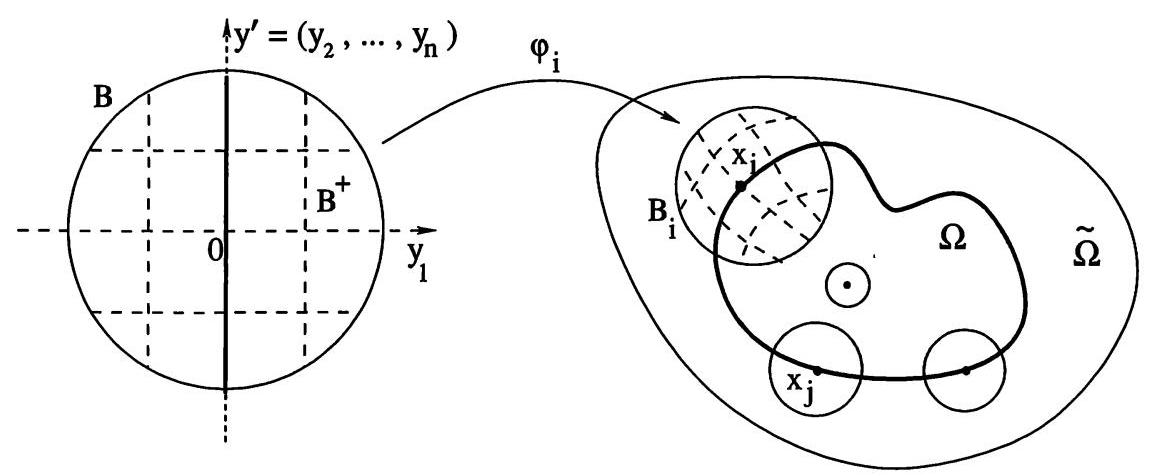
\includegraphics[width=1.0\textwidth]{images/bo_d6ik6nn7aajc739ct1l0_174_168_582_1149_476_0.jpg}
\caption{集合 $\Omega$ 的开覆盖.对每个球 ${B}_{i} = \; B\left( {{x}_{i},{r}_{i}}\right)$ ，存在一个 ${\mathcal{C}}^{1}$ 双射 ${\varphi }_{i}$ ，将单位开球 $B \subset  {\mathbb{R}}^{n}$ 映射到 ${B}_{i}$ .对那些以边界 $\Omega$ 上点为球心的球 ${B}_{i}$ ，正半球 ${B}^{ + } = B \cap  \left\{  {{y}_{1} > 0}\right\}$ 被映射到交集 ${B}_{i} \cap  \Omega$ .}
\label{fig:omega-covering}
\end{figure}

\noindent 2. 为处理一般情形，我们使用单位分解.对每个 $x \in  \overline{\Omega }$ (即 $\Omega$ 的闭包)，选取半径 ${r}_{x} > 0$ ，使得以 $x$ 为中心、半径为 ${r}_{x}0$ 的开球 $B\left( {x,{r}_{x}}\right)$ 满足以下条件:
\begin{itemize}
\item 若 $x \in  \Omega$ ，则 $B\left( {x,{r}_{x}}\right)  \subset  \Omega$ .
\item 若 $x \in  \partial \Omega$ ，则 $B\left( {x,{r}_{x}}\right)  \subset  \widetilde{\Omega }$ .此外，记 $B \doteq  B\left( {0,1}\right)$ 为 ${\mathbb{R}}^{n}$ 中的单位开球，则存在一个 ${\mathcal{C}}^{1}$ 双射 ${\varphi }^{x} : B \mapsto  B\left( {x,{r}_{x}}\right)$ ，其逆映射亦为 ${\mathcal{C}}^{1}$ ，该映射将半球
\[
{B}^{ + } \doteq  \left\{  {y = \left( {{y}_{1},{y}_{2},\ldots ,{y}_{n}}\right) ;\sum_{{i = 1}}^{n}{y}_{i}^{2} < 1,{y}_{1} > 0}\right\}
\]
映射到集合 $B\left( {x,{r}^{x}}\right)  \cap  \Omega$ .
\end{itemize}


当 ${r}_{x} > 0$ 取得足够小时，此类双射的存在性由 $\Omega$ 具有 ${\mathcal{C}}^{1}$ 边界的假设保证.

由于 $\Omega$ 有界，其闭包 $\overline{\Omega }$ 是紧的，故可被有限个球 ${B}_{i} = B\left( {{x}_{i},{r}_{i}}\right) ,i = 1,\ldots ,N$ 覆盖.设 ${\varphi }_{i} : B \mapsto  {B}_{i}$ 为对应的双射.回顾可知 ${\varphi }_{i}$ 将 ${B}^{ + }$ 映射到 ${B}_{i} \cap  \Omega$ .

\noindent 3. 设 ${\eta }_{1},\ldots ,{\eta }_{N}$ 为上述覆盖的光滑单位分解.对每个 $x \in  \Omega$ ，我们有
\begin{equation}\tag{8.41}\label{eq:partition-unity-u}
u\left( x\right)  = \sum_{{i = 1}}^{N}{\eta }_{i}\left( x\right) u\left( x\right) .
\end{equation}

我们将指标集划分为
\[
\{ 1,2,\ldots ,N\}  = \mathcal{I} \cup  \mathcal{J},
\]
其中 $\mathcal{I}$ 包含满足 ${x}_{i} \in  \Omega$ 的指标，而 $\mathcal{J}$ 包含满足 ${x}_{i} \in  \partial \Omega$ 的指标.

对每个 $i \in  \mathcal{J}$ ，有 ${\eta }_{i}u \in  {W}^{1,p}\left( {{B}_{i} \cap  \Omega }\right)$ .因此由定理\ref{thm:weak-derivative-properties}(iv)得 $\left( {{\eta }_{i}u}\right)  \circ  {\varphi }_{i} \in  {W}^{1,p}\left( {B}^{ + }\right)$ .应用在\eqref{eq:extension-reflection}处定义的延拓算子 ${E}^{\sharp }$ ，得到
\[
{E}^{\sharp }\left( {\left( {{\eta }_{i}u}\right)  \circ  {\varphi }_{i}}\right) \; \in  \;{W}^{1,p}\left( {B}^{ + }\right) ,\;{E}^{\sharp }\left( {\left( {{\eta }_{i}u}\right)  \circ  {\varphi }_{i}}\right)  \circ  {\varphi }_{i}^{-1}\; \in  \;{W}^{1,p}\left( {B}_{i}\right) .
\]

将所有这些延拓相加，我们定义
\[
{Eu} \doteq  \sum_{{i \in  \mathcal{I}}}{\eta }_{i}u + \sum_{{i \in  \mathcal{J}}}{E}^{\sharp }\left( {\left( {{\eta }_{i}u}\right)  \circ  {\varphi }_{i}}\right)  \circ  {\varphi }_{i}^{-1}.
\]

现在显然，延拓算子 $E$ 满足所有要求.事实上，(i)由\eqref{eq:partition-unity-u}推出；性质(ii)源于如下事实:对每个 $u \in  {W}^{1,p}\left( \Omega \right)$ ， ${Eu}$ 的支集包含于 $\mathop{\bigcup }\limits_{{i = 1}}^{N}{B}_{i} \subseteq  \widetilde{\Omega }$ ；最后，由于 $E$ 被定义为有限个有界线性算子之和，故存在某个常数 $C$ ，使得估计式(iii)成立.

\end{proof}

\section{嵌入定理}

在一维空间中，若函数 $u : \mathbb{R} \mapsto  \mathbb{R}$ 存在弱导数 ${Du} \in  {L}^{1}\left( \mathbb{R}\right)$ ，则其(在零测集上修改取值后)绝对连续；反之，若 $\Omega  \subseteq  {\mathbb{R}}^{n}$ 且 $n \geq  2$ ，则存在既不连续也不有界的函数 $u \in  {W}^{1,p}\left( \Omega \right)$ .例如函数 $u\left( x\right)  = {\left| x\right| }^{-\gamma }$ 在 $0 < \gamma  < \frac{n - p}{p}$ 时即属此情形.

在偏微分方程或变分法的诸多应用中，理解函数 $u \in \; {W}^{k,p}\left( {\mathbb{R}}^{n}\right)$ 所具有的正则性程度至关重要.我们将证明两个朝此方向的基本结果.

\noindent 1.(Morrey)若 $p > n$ ，则每个函数 $u \in  {W}^{1,p}\left( {\mathbb{R}}^{n}\right)$ (在零测集上修改后)均Hölder连续.

\noindent 2.(Gagliardo-Nirenberg)若 $p < n$ ，则每个函数 $u \in  {W}^{1,p}\left( {\mathbb{R}}^{n}\right)$ 属于空间 ${L}^{{p}^{ * }}\left( {\mathbb{R}}^{n}\right)$ ，且具有更大的指数 ${p}^{ * } = p + \frac{{p}^{2}}{n - p}$ .

在这两种情形下，结果均可表述为嵌入定理:在零测集上修改后，每个函数 $u \in  {W}^{1,p}\left( \Omega \right)$ 亦属于某个其他Banach空间 $X$ ；此处 $X = {C}^{0,\gamma }$ 或 $X = {L}^{q}$ ，其中 $q > p$ 为某常数.基本思路如下:
\begin{enumerate}[(I)]
    \item \allbf{对所有光滑函数证明先验估计.}对任意函数 $u \in  {\mathcal{C}}^{\infty }\left( \Omega \right)  \cap  {W}^{k,p}\left( \Omega \right)$ ，证明 $u$ 亦属于另一Banach空间 $X$ ，且存在仅依赖于 $k,p,\Omega$ 而与 $u$ 无关的常数 $C$ ，使得
\begin{equation}\tag{8.42}\label{eq:embedding-apriori}
\| u{\| }_{X}\; \leq  \;C\| u{\| }_{{W}^{k,p}}\;\forall\,u \in  {\mathcal{C}}^{\infty }\left( \Omega \right)  \cap  {W}^{k,p}\left( \Omega \right) \;.
\end{equation}
    \item \allbf{利用连续性将嵌入推广至整个空间.}由于 ${\mathcal{C}}^{\infty }$ 在 ${W}^{k,p}$ 中稠密，故对每个 $u \in  {W}^{k,p}\left( \Omega \right)$ ，可找到一列函数 ${u}_{n} \in  {\mathcal{C}}^{\infty }\left( \Omega \right)$ 使得 $\norm{u - {u}_{n}}_{{W}^{k,p}} \rightarrow  0$ 成立.由\eqref{eq:embedding-apriori}式，
    \[
    \limsup_{{m,n \rightarrow  \infty }}{\norm{u_{m} - {u}_{n}}}_{X} \leq  \limsup_{{m,n \rightarrow  \infty }}C{\norm{u_{m} - {u}_{n}}}_{{W}^{k,p}} = 0.
    \]
    因此，函数 ${u}_{n}$ 在空间 $X$ 中也构成Cauchy列.由完备性可知， ${u}_{n} \rightarrow  \widetilde{u}$ 对某个 $\widetilde{u} \in  X$ 成立.注意到对几乎处处的 $x \in  \Omega$ 有 $\widetilde{u}\left( x\right)  = u\left( x\right)$ ，故可推出:在测度为零的集合 $\mathcal{N} \subset  \Omega$ 上作适当修改后，每个函数 $u \in  {W}^{k,p}\left( \Omega \right)$ 也属于空间 $X$ .
\end{enumerate}



\subsection{莫雷不等式}

本节证明:若 $u \in  {W}^{1,p}\left( {\mathbb{R}}^{n}\right)$ ，其中指数 $p$ 大于空间维数 $n$ ，则 $u$ 几乎处处等于一个Hölder连续函数.
\begin{theorem}[莫雷不等式]\label{thm:morrey-inequality}
设 $n < p < \infty$ ，并令 $\gamma  \doteq  1 - \frac{n}{p} > 0$ .则存在仅依赖于 $p$ 和 $n$ 的常数 $C$ ，使得
\begin{equation}\tag{8.43}\label{eq:morrey-inequality}
\| u{\| }_{{\mathcal{C}}^{0,\gamma }\left( {\mathbb{R}}^{n}\right) }\; \leq  \;C\| u{\| }_{{W}^{1,p}\left( {\mathbb{R}}^{n}\right) }
\end{equation}

对每个 $u \in  {\mathcal{C}}^{1}\left( {\mathbb{R}}^{n}\right)  \cap  {W}^{1,p}\left( {\mathbb{R}}^{n}\right)$ 成立.
\end{theorem}

\begin{proof}
在给出严格证明之前，先概述其思想.由函数$u$的梯度满足的一个积分估计，例如
\begin{equation}\tag{8.44}\label{eq:morrey-gradient-Lp-bound}
{\int }_{{\mathbb{R}}^{n}}{\left| \nabla u\left( x\right) \right| }^{p}{\d x} \leq  {C}_{0}
\end{equation}
我们希望得到如下形式的逐点估计:
\begin{equation}\tag{8.45}\label{eq:morrey-holder-target}
\left| {u\left( y\right)  - u\left( {y}^{\prime }\right) }\right|  \leq  {C}_{1}{\left| y - {y}^{\prime }\right| }^{\gamma }\;\forall\,y,{y}^{\prime } \in  {\mathbb{R}}^{n}.
\end{equation}

\begin{figure}[htbp]
\centering
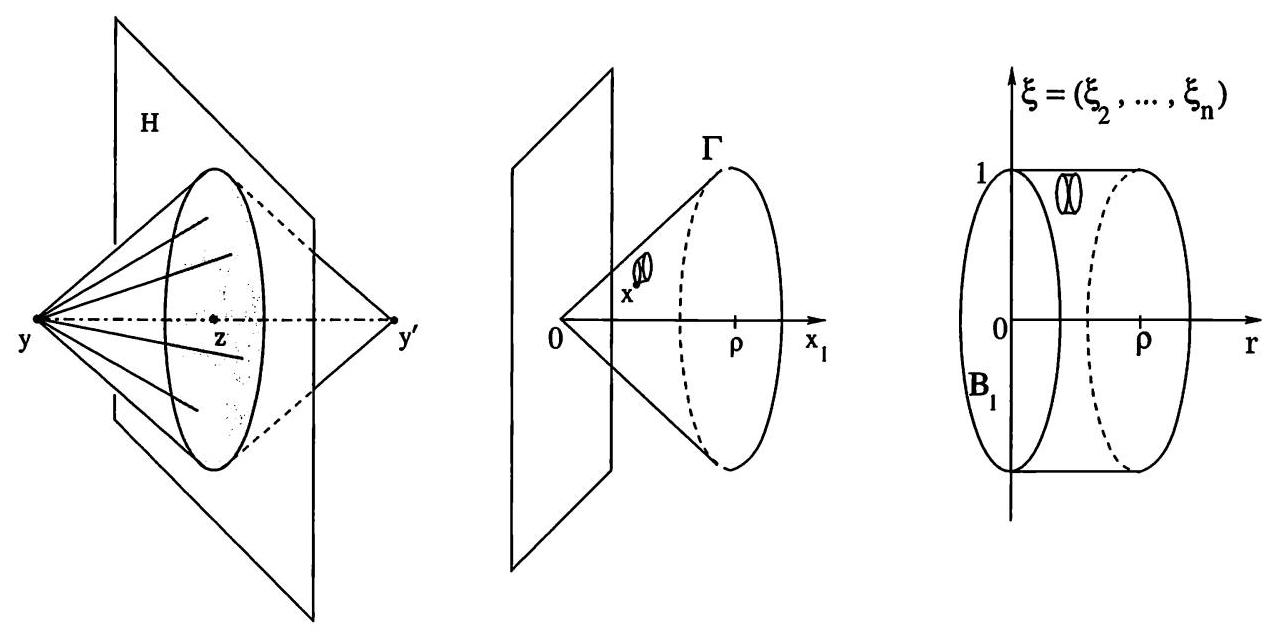
\includegraphics[width=0.95\textwidth]{images/bo_d6ik6nn7aajc739ct1l0_177_106_234_1282_634_0.jpg}
\caption{莫雷不等式的证明.左:在垂直于向量 $y - {y}^{\prime }$ 的超平面 $H$ 内，以中点 $z$ 为中心、位于该平面内的 $\left( {n - 1}\right)$ 维球(阴影区域)上取函数 $u$ 的平均值，并将 $u\left( y\right)$ 与 $u\left( {y}^{\prime }\right)$ 的值分别与之比较.中与右:锥 $\Gamma$ 中一点 $x$ 用坐标 $\left( {r,\xi }\right)  \in  \left(  {0,\rho }\right)   \times  {B}_{1}$ 表示.}
\label{fig:morrey-proof}
\end{figure}

为实现\eqref{eq:morrey-holder-target}，一种自然尝试是写作
\begin{equation}\tag{8.46}\label{eq:morrey-segment-bound}
    \setjot[-2]\begin{aligned}
        \left| {u\left( y\right)  - u\left( {y}^{\prime }\right) }\right|  &= \left| {{\int }_{0}^{1}\left(  {\frac{d}{d\theta }u\left( {{\theta y} + \left( {1 - \theta }\right) {y}^{\prime }}\right) }\right)  {d\theta }}\right|\\
        &\leq  {\int }_{0}^{1}\left| {\nabla u\left( {{\theta y} + \left( {1 - \theta }\right) {y}^{\prime }}\right) }\right| \left| {y - {y}^{\prime }}\right| {d\theta }.
    \end{aligned}
\end{equation}

然而，\eqref{eq:morrey-segment-bound}式右端积分仅涉及 $\nabla u$ 在连接 $y$ 与 ${y}^{\prime }$ 的线段上的取值.若空间维数为 $n > 1$ ，则该线段测度为零；因此即使\eqref{eq:morrey-gradient-Lp-bound}中的积分很小，\eqref{eq:morrey-segment-bound}式右端积分仍可能任意大.为克服这一困难，我们将 $u\left( y\right) ,u\left( {y}^{\prime }\right)$ 二者均与函数 $u$ 在以中点 $z = \frac{y + {y}^{\prime }}{2}$ 为中心的 $\left( {n - 1}\right)$ 维球上的平均值 ${u}_{A}$ 进行比较，如图\ref{fig:morrey-proof}(左)所示.注意，差值 $\left| {u\left( y\right)  - {u}_{A}}\right|$ 可通过在 $n$ 维锥上对 $\left| {\nabla u}\right|$ 积分来估计.由此便可利用界\eqref{eq:morrey-gradient-Lp-bound}.

\noindent 1. 现在开始证明，并先作一预备计算.在 ${\mathbb{R}}^{n}$ 上考虑锥
\[
\Gamma  \doteq  \left\{  {x = \left( {{x}_{1},{x}_{2},\ldots ,{x}_{n}}\right) ;\;\sum_{{j = 2}}^{n}{x}_{j}^{2} \leq  {x}_{1}^{2},\;0 < {x}_{1} < \rho }\right\}
\]
及函数
\begin{equation}\tag{8.47}\label{eq:morrey-psi}
\psi \left( x\right)  = \frac{1}{{x}_{1}^{n - 1}}.
\end{equation}

令 $q = \frac{p}{p - 1}$ 为 $p$ 的共轭指数，即满足 $\frac{1}{p} + \frac{1}{q} = 1$ .我们计算
{\setjot[0]\begin{align*}
    \| \psi {\| }_{{L}^{q}\left( \Gamma \right) }^{q} &= {\int }_{\Gamma }{\left( \frac{1}{{x}_{1}^{n - 1}}\right) }^{q}{\d x} = {\int }_{0}^{\rho }{c}_{n - 1}{x}_{1}^{n - 1}{\left( \frac{1}{{x}_{1}^{n - 1}}\right) }^{q}\d x_{1}\\
    &= {c}_{n - 1}{\int }_{0}^{\rho }{s}^{\left( {n - 1}\right) \left( {1 - q}\right) }{\d s}
\end{align*}}
其中常数 ${c}_{n - 1}$ 给出 ${\mathbb{R}}^{n - 1}$ 中单位球的体积.因此， $\psi  \in  {L}^{q}\left( \Gamma \right)$ 当且仅当 $n < p$ .此时，
\begin{equation}\tag{8.48}\label{eq:morrey-psi-norm}
\| \psi {\| }_{{L}^{q}\left( \Gamma \right) } = {\left( {c}_{n - 1}{\int }_{0}^{\rho }{s}^{-\frac{n - 1}{p - 1}}\d s\right) }^{\frac{1}{q}} = c{\left( {\rho }^{\frac{p - n}{p - 1}}\right) }^{\frac{p - 1}{p}} = c{\rho }^{\frac{p - n}{p}},
\end{equation}
其中常数 $c$ 仅依赖于 $n$ 和 $p$ .

\noindent 2. 考虑任意两个不同点 $y,{y}^{\prime } \in  {\mathbb{R}}^{n}$ .令 $\rho  \doteq  \frac{1}{2}\left| {y - {y}^{\prime }}\right|$ .过中点 $z \doteq  \frac{y + {y}^{\prime }}{2}$ 且垂直于向量 $y - {y}^{\prime }$ 的超平面方程为
\[
H = \left\{  {x \in  {\mathbb{R}}^{n};\left\langle  {x - z,y - {y}^{\prime }}\right\rangle   = 0}\right\}  .
\]

在 $H$ 内，考虑以 $z$ 为中心、半径为 $\rho$ 的 $\left( {n - 1}\right)$ 维球，
\[
{B}_{\rho } \doteq  \{ x \in  H;\left| {x - z}\right|  < \rho \} .
\]

记 ${u}_{A}$ 为 $u$ 在球 ${B}_{\rho }$ 上的平均值，则差值 $\left| {u\left( y\right)  - u\left( {y}^{\prime }\right) }\right|$ 将被估计为
\begin{equation}\tag{8.49}\label{eq:morrey-split}
\left| {u\left( y\right)  - u\left( {y}^{\prime }\right) }\right|  \leq  \left| {u\left( y\right)  - {u}_{A}}\right|  + \left| {{u}_{A} - u\left( {y}^{\prime }\right) }\right| .
\end{equation}

\noindent 3. 通过坐标平移与旋转，可假设
\[
y = \left( {0,\ldots ,0}\right)  \in  {\mathbb{R}}^{n},\;\quad {B}_{\rho } = \left\{  {x = \left( {{x}_{1},{x}_{2},\ldots ,{x}_{n}}\right) ;{x}_{1} = \rho ,\sum_{{i = 2}}^{n}{x}_{i}^{2} \leq  {\rho }^{2}}\right\}  .
\]

为计算平均值 ${u}_{A}$ ，令 ${B}_{1}$ 为 ${\mathbb{R}}^{n - 1}$ 中的单位球，并令 ${c}_{n - 1}$ 为其 $\left( {n - 1}\right)$ 维测度.锥体 $\Gamma$ 中的点将用另一套坐标系描述.对具有坐标 $\left( {r,\xi }\right)  = \left( {r,{\xi }_{2},\ldots ,{\xi }_{n}}\right)  \in  \left(  {0,\rho }\right)   \times  {B}_{1}$ 的点，关联其具有分量的点 $x\left( {r,\xi }\right)  \in  \Gamma$
\begin{equation}\tag{8.50}\label{eq:morrey-cone-coords}
\left( {{x}_{1},{x}_{2},\ldots ,{x}_{n}}\right)  = \left( {r,{r\xi }}\right)  = \left( {r,r{\xi }_{2},\ldots ,r{\xi }_{n}}\right) .
\end{equation}

定义 $U\left( {r,\xi }\right)  = u\left( {r,{r\xi }}\right)$ ，并注意到对每个 $\xi$ 均有 $U\left( {0,\xi }\right)  = u\left( 0\right)$ .

因此
\[
U\left( {\rho ,\xi }\right)  = U\left( {0,\xi }\right)  + {\int }_{0}^{\rho }\left(  {\frac{\partial }{\partial r}U\left( {r,\xi }\right) }\right)  {\d r},
\]
\begin{equation}\tag{8.51}\label{eq:morrey-uA-average}
{u}_{A} - u\left( 0\right)  = \frac{1}{{c}_{n - 1}}{\int }_{{B}_{1}}\left( {{\int }_{0}^{\rho }\left(  {\frac{\partial }{\partial r}U\left( {r,\xi }\right) }\right)  {\d r}}\right) {\d \xi }.
\end{equation}

我们现在作变量替换，将积分\eqref{eq:morrey-uA-average}在 $\left(  {0,\rho }\right)   \times  {B}_{1}$ 上的积分变换为在锥体 $\Gamma$ 上的积分.计算变换\eqref{eq:morrey-cone-coords}的雅可比矩阵，得其行列式为 ${r}^{n - 1}$ ；故
\[
\d x_{1}\d x_{2}\cdots \d x_{n} = {r}^{n - 1}\d{r}\d{\xi }_{2}\cdots \d{\xi }_{n}.
\]

此外，由于 $\left| \xi \right|  \leq  1$ ，函数 $u$ 沿向量 $\left( {1,{\xi }_{2},\ldots ,{\xi }_{n}}\right)$ 方向的方向导数被估计为
\begin{equation}\tag{8.52}\label{eq:morrey-dUr-bound}
\left| {\frac{\partial }{\partial r}U\left( {r,\xi }\right) }\right|  = \left| {{u}_{{x}_{1}} + \sum_{{i = 2}}^{n}{\xi }_{i}{u}_{{x}_{i}}}\right|  \leq  2\left| {\nabla u\left( {r,\xi }\right) }\right| .
\end{equation}

在\eqref{eq:morrey-uA-average}中代入\eqref{eq:morrey-dUr-bound}，并利用函数 $\psi \left( x\right)  \doteq  {x}_{1}^{1 - n}$ 的 ${L}^{q}$ 范数估计\eqref{eq:morrey-psi-norm}，得到
\begin{equation}\tag{8.53}\label{eq:morrey-uA-bound}
    {\setjot[0]\begin{aligned}
        \left| {{u}_{A} - u\left( 0\right) }\right|  &\leq  \frac{2}{{c}_{n - 1}}{\int }_{\Gamma }\frac{1}{{x}_{1}^{n - 1}}\left| {\nabla u\left( x\right) }\right| {\d x}\\
        &\leq  \frac{2}{{c}_{n - 1}}\| \psi {\| }_{{L}^{q}\left( \Gamma \right) }\| \nabla u{\| }_{{L}^{p}\left( \Gamma \right) }\;\quad \left( {q = \frac{p}{p - 1}}\right)\\
        &\leq  C{\rho }^{\frac{p - n}{p}}\| u{\| }_{{W}^{1,p}\left( {\mathbb{R}}^{n}\right) }.
    \end{aligned}}
\end{equation}
其中 $C$ 为某常数.注意最后两步分别由 Hölder 不等式及\eqref{eq:morrey-psi-norm}得出.

\noindent 4. 利用\eqref{eq:morrey-uA-bound}估计\eqref{eq:morrey-split}右端每一项，并回顾 $\rho  = \frac{1}{2}\left| {y - {y}^{\prime }}\right|$ ，我们得出
\begin{equation}\tag{8.54}\label{eq:morrey-holder}
\left| {u\left( y\right)  - u\left( {y}^{\prime }\right) }\right|  \leq  {2C}{\left( \frac{\left| y - {y}^{\prime }\right| }{2}\right) }^{\frac{p - n}{p}}\| u{\| }_{{W}^{1,p}\left( {\mathbb{R}}^{n}\right) }.
\end{equation}

这表明 $u$ 是指数为 $\gamma  = \frac{p - n}{p}$ 的 Hölder 连续函数.

\noindent 5. 为估计 $\mathop{\sup }\limits_{y}\left| {u\left( y\right) }\right|$ ，我们注意到，由\eqref{eq:morrey-holder}，存在某常数 ${C}_{1}$ ，使得
\[
\left| {u\left( y\right) }\right|  \leq  \left| {u\left( x\right) }\right|  + {C}_{1}\| u{\| }_{{W}^{1,p}\left( {\mathbb{R}}^{n}\right) }\;\forall\,x \in  B\left( {y,1}\right) .
\]

对以 $y$ 为中心、半径为1的球上右侧表达式取平均，得到
\begin{equation}\tag{8.55}\label{eq:morrey-sup-estimate}
\left| {u\left( y\right) }\right|  \leq  {\int }_{B\left( {y,1}\right) }\left| {u\left( x\right) }\right| {\d x} + {C}_{1}\| u{\| }_{{W}^{1,p}\left( {\mathbb{R}}^{n}\right) } \leq  {C}_{2}\| u{\| }_{{L}^{p}\left( {\mathbb{R}}^{n}\right) } + {C}_{1}\| u{\| }_{{W}^{1,p}\left( {\mathbb{R}}^{n}\right) }.
\end{equation}

\noindent 6. 综合\eqref{eq:morrey-holder}--\eqref{eq:morrey-sup-estimate}可得
\[
\| u{\| }_{{\mathcal{C}}^{0,\gamma }\left( {\mathbb{R}}^{n}\right) } \doteq  \mathop{\sup }\limits_{y}\left| {u\left( y\right) }\right|  + \mathop{\sup }\limits_{{y \neq  {y}^{\prime }}}\frac{\left| u\left( y\right)  - u\left( {y}^{\prime }\right) \right| }{{\left| y - {y}^{\prime }\right| }^{\gamma }} \leq  C\| u{\| }_{{W}^{1,p}\left( {\mathbb{R}}^{n}\right) },
\]
其中常数 $C$ 仅依赖于 $p$ 和 $n$ .
\end{proof}

由于 ${\mathcal{C}}^{\infty }$ 在 ${W}^{1,p}$ 中稠密，由定理\ref{thm:morrey-inequality}可得

\begin{corollary}[嵌入]\label{cor:morrey-embedding}
设 $\Omega  \subset  {\mathbb{R}}^{n}$ 为具有 ${\mathcal{C}}^{1}$ 边界的有界开集.假设 $n < p < \infty$ ，并令 $\gamma  \doteq  1 - \frac{n}{p} > 0$ .则每个函数 $f \in  {W}^{1,p}\left( \Omega \right)$ 几乎处处等于某个函数 $\widetilde{f} \in  {\mathcal{C}}^{0,\gamma }\left( \Omega \right)$ .此外，存在常数 $C$ ，使得
\begin{equation}\tag{8.56}\label{eq:morrey-embedding}
\| \widetilde{f}{\| }_{{\mathcal{C}}^{0,\gamma }} \leq  C\| f{\| }_{{W}^{1,p}}\;\forall\,f \in  {W}^{1,p}\left( \Omega \right) .
\end{equation}
\end{corollary}

\begin{proof}
1. 令 $\widetilde{\Omega } \doteq  \left\{  {x \in  {\mathbb{R}}^{n};d\left( {x,\Omega }\right)  < 1}\right\}$ 为集合 $\Omega$ 的半径为1的开邻域.由定理\ref{thm:extension-operator}可知，存在有界延拓算子 $E$ ，它将每个函数 $f \in  {W}^{1,p}\left( \Omega \right)$ 延拓为支集包含于 $\widetilde{\Omega }$ 内的函数 ${Ef} \in  {W}^{1,p}\left( {\mathbb{R}}^{n}\right)$ .

\noindent 2. 由于 ${\mathcal{C}}^{1}\left( {\mathbb{R}}^{n}\right)$ 在 ${W}^{1,p}\left( {\mathbb{R}}^{n}\right)$ 中稠密，可取一列函数 ${g}_{n} \in  {\mathcal{C}}^{1}\left( {\mathbb{R}}^{n}\right)$ 在 ${W}^{1,p}\left( {\mathbb{R}}^{n}\right)$ 中收敛于 ${Ef}$ .由定理\ref{thm:morrey-inequality}
\[
\limsup_{{m,n \rightarrow  \infty }}{\norm{g_{m} - {g}_{n}}}_{{C}^{0,\gamma }\left( {\mathbb{R}}^{n}\right) } \leq  C\limsup_{{m,n \rightarrow  \infty }}{\norm{g_{m} - {g}_{n}}}_{{W}^{1,p}\left( {\mathbb{R}}^{n}\right) } = 0.
\]

这表明序列 ${\left( {g}_{n}\right) }_{n \geq  1}$ 在空间 ${\mathcal{C}}^{0,\gamma }$ 中亦为Cauchy列.因此它一致收敛于某个极限函数 $g \in  {C}^{0,\gamma }\left( {\mathbb{R}}^{n}\right)$ (对 $x \in  {\mathbb{R}}^{n}$ 一致).

\noindent 3. 由于 ${g}_{n} \rightarrow  {Ef}$ 在 ${W}^{1,p}\left( {\mathbb{R}}^{n}\right)$ 中，故对$\text{a.e.}\; x \in  {\mathbb{R}}^{n}$ 亦有 $g\left( x\right)  = \left( {Ef}\right) \left( x\right)$ .特别地，对$\text{a.e.}\;x \in  \Omega$ 有 $g\left( x\right)  = f\left( x\right)$ .又因延拓算子 $E$ 有界，由式\eqref{eq:morrey-inequality}可推出\eqref{eq:morrey-embedding}.
\end{proof}

\begin{remark}\label{rem:morrey-embedding-Rn}
若 $\Omega  = {\mathbb{R}}^{n}$ ，推论\ref{cor:morrey-embedding}的结论仍成立.
\end{remark}

\subsection{Gagliardo--Nirenberg不等式}

接下来我们研究 $1 \leq  p < n$ 的情形.定义 $p$ 的\bluebf{Soblev共轭}为
\begin{equation}\tag{8.57}\label{eq:p-star}
{p}^{ * } \doteq  \frac{np}{n - p} > p.
\end{equation}

注意， ${p}^{ * }$ 不仅依赖于 $p$ ，还依赖于空间的维数 $n$ :
\begin{equation}\tag{8.58}\label{eq:p-star-reciprocal}
\frac{1}{{p}^{ * }} = \frac{1}{p} - \frac{1}{n}
\end{equation}

作为预备知识，我们介绍广义Hölder不等式的一个有用应用；参见附录中的(A.26).设给定非负函数 $n - 1$  ${g}_{1},{g}_{2},\ldots ,{g}_{n - 1} \in  {L}^{1}\left( \Omega \right)$ .由于对每个 $i$ 均有 ${g}_{i}^{\frac{1}{n - 1}} \in  {L}^{n - 1}\left( \Omega \right)$，应用广义Hölder不等式可得
\begin{equation}\tag{8.59}\label{eq:generalized-holder-application}
{\int }_{\Omega }{g}_{1}^{\frac{1}{n - 1}}{g}_{2}^{\frac{1}{n - 1}}\cdots {g}_{n - 1}^{\frac{1}{n - 1}}{\d s} \leq  \mathop{\prod }\limits_{{i = 1}}^{{n - 1}}{\norm{g_{i}^{\frac{1}{n - 1}}}}_{{L}^{n - 1}} = \mathop{\prod }\limits_{{i = 1}}^{{n - 1}}{\norm{g}_{i}}_{{L}^{1}}^{\frac{1}{n - 1}}.
\end{equation}

\begin{theorem}[Gagliardo--Nirenberg不等式]\label{thm:gagliardo-nirenberg}
假设 $1 \leq  p < n$ .则存在仅依赖于 $p$ 和 $n$ 的常数 $C$ ，使得
\begin{equation}\tag{8.60}\label{eq:gagliardo-nirenberg}
\| f{\| }_{{L}^{{p}^{ * }}\left( {\mathbb{R}}^{n}\right) }\; \leq  \;C\| \nabla f{\| }_{{L}^{p}\left( {\mathbb{R}}^{n}\right) },\;\forall\,\;f \in  {C}_{c}^{1}\left( {\mathbb{R}}^{n}\right) .
\end{equation}
\end{theorem}

\begin{figure}[htbp]
\centering
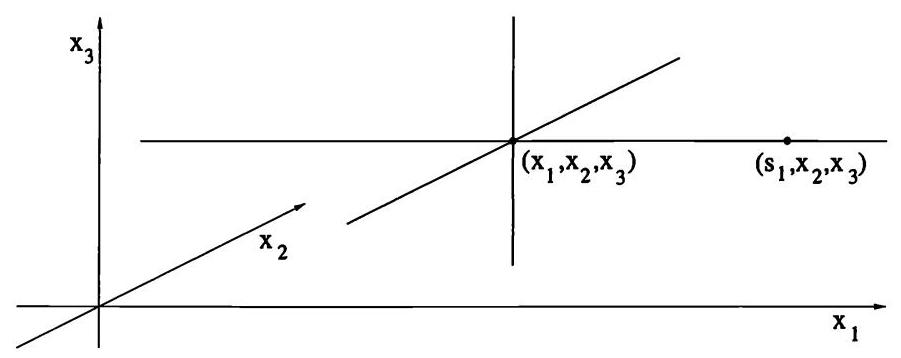
\includegraphics[width=0.8\textwidth]{images/bo_d6ik6nn7aajc739ct1l0_181_291_1364_901_358_0.jpg}
\caption{证明加利亚尔多--尼伦伯格不等式.积分 ${\int }_{-\infty }^{\infty }\left| {{D}_{{x}_{1}}f\left( {{s}_{1},{x}_{2},{x}_{3}}\right) }\right| \d s_{1}$ 依赖于 ${x}_{2},{x}_{3}$ 但不依赖于 ${x}_{1}$ .类似地，积分 ${\int }_{-\infty }^{\infty }\left| {{D}_{{x}_{2}}f\left( {{x}_{1},{s}_{2},{x}_{3}}\right) }\right| \d s_{2}$ 依赖于 ${x}_{1},{x}_{3}$ 但不依赖于 ${x}_{2}$ .}
\label{fig:gn-proof}
\end{figure}

\begin{proof}
1. 对每个 $i \in  \{ 1,\ldots ,n\}$ 及每一点 $x = \left( {{x}_{1},\ldots ,{x}_{i},\ldots ,{x}_{n}}\right)  \in \; {\mathbb{R}}^{n}$ ，由于 $f$ 具有紧支集，可写为
\[
f\left( {{x}_{1},\ldots ,{x}_{i},\ldots ,{x}_{n}}\right)  = {\int }_{-\infty }^{{x}_{i}}{D}_{{x}_{i}}f\left( {{x}_{1},\ldots ,{s}_{i},\ldots ,{x}_{n}}\right) \d s_{i}.
\]

进而得到
\[
\left| {f\left( {{x}_{1},\ldots ,{x}_{n}}\right) }\right|  \leq  {\int }_{-\infty }^{\infty }\left| {{D}_{{x}_{i}}f\left( {{x}_{1},\ldots ,{s}_{i},\ldots ,{x}_{n}}\right) }\right| \d s_{i},\;1 \leq  i \leq  n,
\]
\begin{equation}\tag{8.61}\label{eq:gn-pointwise}
{\left| f\left( x\right) \right| }^{\frac{n}{n - 1}} \leq  \mathop{\prod }\limits_{{i = 1}}^{n}{\left( {\int }_{-\infty }^{\infty }\left| {D}_{{x}_{i}}f\left( {x}_{1},\ldots ,{s}_{i},\ldots ,{x}_{n}\right) \right| \d s_{i}\right) }^{\frac{1}{n - 1}}.
\end{equation}

现对\eqref{eq:gn-pointwise}关于 ${x}_{1}$ 积分.注意右侧第一因子不依赖于 ${x}_{1}$ .该因子表现如常数，可提出积分号外.剩余 $n - 1$ 个因子的乘积则利用\eqref{eq:generalized-holder-application}处理.由此得到\eqref{eq:gn-integrate-x1}
\begin{equation}\tag{8.62}\label{eq:gn-integrate-x1}
\begin{aligned}
&{\int }_{-\infty }^{\infty }{\left| f\right| }^{\frac{n}{n - 1}}\d x_{1}\\
&\leq  {\left( {\int }_{-\infty }^{\infty }\left| {D}_{{x}_{1}}f\right| \d s_{1}\right) }^{\frac{1}{n - 1}}{\int }_{-\infty }^{\infty }\mathop{\prod }\limits_{{i = 2}}^{n}{\left( {\int }_{-\infty }^{\infty }\left| {D}_{{x}_{i}}f\right| \d s_{i}\right) }^{\frac{1}{n - 1}}\d x_{1} \\
&\leq  {\left( {\int }_{-\infty }^{\infty }\left| {D}_{{x}_{1}}f\right| \d s_{1}\right) }^{\frac{1}{n - 1}}\mathop{\prod }\limits_{{i = 2}}^{n}{\left( {\int }_{-\infty }^{\infty }{\int }_{-\infty }^{\infty }\left| {D}_{{x}_{i}}f\right| \d s_{i}\d x_{1}\right) }^{\frac{1}{n - 1}}.
\end{aligned}
\end{equation}
注意第二个不等式是将广义Hölder不等式应用于 $n - 1$ 个函数 ${g}_{i} = {\int }_{-\infty }^{\infty }\left| {{D}_{{x}_{i}}f}\right| \d s_{i},i = 2,\ldots ,n$ 所得.

现对\eqref{eq:gn-integrate-x1}两边关于 ${x}_{2}$ 积分.注意\eqref{eq:gn-integrate-x1}右侧乘积中出现的一个因子不依赖于变量 ${x}_{2}$ (即涉及关于 ${s}_{2}$ 积分的那个因子).该因子表现如常数，可提出积分号外.剩余 $n - 2$ 个因子的乘积再次用Hölder不等式估计.由此得到
\begin{equation}\tag{8.63}\label{eq:gn-integrate-x2}
\begin{aligned}
&{\int }_{-\infty }^{\infty }{\int }_{-\infty }^{\infty }{\left| f\right| }^{\frac{n}{n - 1}}\d x_{1}\d x_{2}\\
&\leq  {\left( {\int }_{-\infty }^{\infty }{\int }_{-\infty }^{\infty }\left| {D}_{{x}_{1}}f\right| \d x_{1}\d x_{2}\right) }^{\frac{1}{n - 1}}{\left( {\int }_{-\infty }^{\infty }{\int }_{-\infty }^{\infty }\left| {D}_{{x}_{2}}f\right| \d x_{1}\d x_{2}\right) }^{\frac{1}{n - 1}} \\
&\quad\times  \mathop{\prod }\limits_{{i = 3}}^{n}{\left( {\int }_{-\infty }^{\infty }{\int }_{-\infty }^{\infty }{\int }_{-\infty }^{\infty }\left| {D}_{{x}_{i}}f\right| \d s_{i}\d x_{1}\d x_{2}\right) }^{\frac{1}{n - 1}}.
\end{aligned}
\end{equation}

依同样方式继续，经过 $n$ 次积分后得到
\begin{equation}\tag{8.64}\label{eq:gn-integrate-xn}
\begin{aligned}
&{\int }_{-\infty }^{\infty }\cdots {\int }_{-\infty }^{\infty }{\left| f\right| }^{\frac{n}{n - 1}}\d x_{1}\cdots \d x_{n}\\
&\leq  \mathop{\prod }\limits_{{i = 1}}^{n}{\left( {\int }_{-\infty }^{\infty }\cdots {\int }_{-\infty }^{\infty }\left| {D}_{{x}_{i}}f\right| \d x_{1}\cdots \d x_{n}\right) }^{\frac{1}{n - 1}} \\
&\leq  {\left( {\int }_{{\mathbb{R}}^{n}}\left| \nabla f\right| \d x\right) }^{\frac{n}{n - 1}}.
\end{aligned}
\end{equation}

这已蕴含
\begin{equation}\tag{8.65}\label{eq:gn-p1-case}
\| f{\| }_{{L}^{n/\left( {n - 1}\right) }} = {\left( {\int }_{{\mathbb{R}}^{n}}{\left| f\right| }^{\frac{n}{n - 1}}\d x\right) }^{\frac{n - 1}{n}} \leq  {\int }_{{\mathbb{R}}^{n}}\left| {\nabla f}\right| {\d x},
\end{equation}

从而在 $p = 1$ 且 ${p}^{ * } = \frac{n}{n - 1}$ 的情形下证得该定理.

\noindent 2. 为涵盖 $1 < p < n$ 的一般情形，将\eqref{eq:gn-p1-case}应用于函数
\begin{equation}\tag{8.66}\label{eq:gn-g-definition}
 g \doteq  {\left| f\right| }^{\beta }\;\text{ with }\;\beta  \doteq  \frac{p\left( {n - 1}\right) }{n - p}.
\end{equation}

利用标准Hölder不等式，可得\eqref{eq:gn-holder}
\begin{equation}\tag{8.67}\label{eq:gn-holder}
\begin{aligned}
{\left( {\int }_{{\mathbb{R}}^{n}}{\left| f\right| }^{\frac{\beta n}{n - 1}}\d x\right) }^{\frac{n - 1}{n}}
&\leq  {\int }_{{\mathbb{R}}^{n}}\beta {\left| f\right| }^{\beta  - 1}\left| {\nabla f}\right| {\d x} \\
&\leq  \beta {\left( {\int }_{{\mathbb{R}}^{n}}{\left| f\right| }^{\frac{\left( {\beta  - 1}\right) p}{p - 1}}\d x\right) }^{\frac{p - 1}{p}}{\left( {\int }_{{\mathbb{R}}^{n}}{\left| \nabla f\right| }^{p}\d x\right) }^{\frac{1}{p}}.
\end{aligned}
\end{equation}

$\beta$ 在\eqref{eq:gn-g-definition}中的选取给出
\[
\frac{\left( {\beta  - 1}\right) p}{p - 1} = \frac{\beta n}{n - 1} = \frac{np}{n - p} = {p}^{ * }.
\]

因此，由\eqref{eq:gn-holder}可得
\[
{\left( {\int }_{{\mathbb{R}}^{n}}{\left| f\right| }^{{p}^{ * }}\d x\right) }^{\frac{n - 1}{n}} \leq  \beta {\left( {\int }_{{\mathbb{R}}^{n}}{\left| f\right| }^{{p}^{ * }}\d x\right) }^{\frac{p - 1}{p}}{\left( {\int }_{{\mathbb{R}}^{n}}{\left| \nabla f\right| }^{p}\d x\right) }^{\frac{1}{p}}.
\]

注意到 $\frac{n - 1}{n} - \frac{p - 1}{p} = \frac{n - p}{np} = \frac{1}{{p}^{ * }}$ ，故可得
\[
{\left( {\int }_{{\mathbb{R}}^{n}}{\left| f\right| }^{{p}^{ * }}\d x\right) }^{\frac{1}{{p}^{ * }}} \leq  C{\left( {\int }_{{\mathbb{R}}^{n}}{\left| \nabla f\right| }^{p}\d x\right) }^{\frac{1}{p}}.
\]
\end{proof}

若区域 $\Omega  \subset  {\mathbb{R}}^{n}$ 有界，则对任意 $q \in  \left(  {1,{p}^{ * }}\right)$ ，均有 ${L}^{q}\left( \Omega \right)  \subseteq  {L}^{{p}^{ * }}\left( \Omega \right)$ .由定理\ref{thm:gagliardo-nirenberg}可得

\begin{corollary}[嵌入]\label{cor:gn-embedding}
设 $\Omega  \subset  {\mathbb{R}}^{n}$ 是具有 ${\mathcal{C}}^{1}$ 边界的有界开区域，且假设 $1 \leq  p < n$ .则对任意满足 ${p}^{ * } \doteq  \frac{np}{n - p}$ 的 $q \in  \left(  {1,{p}^{ * }}\right)$ ，存在常数 $C$ ，使得
\begin{equation}\tag{8.68}\label{eq:gn-embedding}
\| f{\| }_{{L}^{q}\left( \Omega \right) }\; \leq  \;C\| f{\| }_{{W}^{1,p}\left( \Omega \right) }\;\forall\,\;f \in  {W}^{1,p}\left( \Omega \right) \;.
\end{equation}
\end{corollary}

\begin{proof}
令 $\widetilde{\Omega } \doteq  \left\{  {x \in  {\mathbb{R}}^{n};d\left( {x,\Omega }\right)  < 1}\right\}$ 为集合 $\Omega$ 的半径为一的开邻域.由定理\ref{thm:extension-operator}，存在有界延拓算子 $E : {W}^{1,p}\left( \Omega \right)  \mapsto  {W}^{1,p}\left( {\mathbb{R}}^{n}\right)$ ，其性质为:对任意 $f \in  {W}^{1,p}\left( \Omega \right)$ ， ${Ef}$ 的支集包含于 $\widetilde{\Omega }$ 内.将定理\ref{thm:gagliardo-nirenberg}应用于 ${Ef}$ ，可得(对适当常数 ${C}_{1},{C}_{2},{C}_{3}$ )
\[
\| f{\| }_{{L}^{q}\left( \Omega \right) }\; \leq  \;{C}_{1}\| f{\| }_{{L}^{{p}^{ * }}\left( \Omega \right) }\; \leq  \;{C}_{2}\| {Ef}{\| }_{{L}^{{p}^{ * }}\left( {\mathbb{R}}^{n}\right) }\; \leq  \;{C}_{3}\| f{\| }_{{W}^{1,p}\left( \Omega \right) }.
\]
\end{proof}

\subsection{高阶 Soblev 估计}

设 $\Omega  \subset  {\mathbb{R}}^{n}$ 是具有 ${\mathcal{C}}^{1}$ 边界的有界开集，且设 $u \in  {W}^{k,p}\left( \Omega \right)$ .称
\[
k - \frac{n}{p}
\]
为 $u$ 的“净光滑性”.如图\ref{fig:net-smoothness}所示，令 $m$ 为此数的整数部分， $0 \leq  \gamma  < 1$ 为其小数部分，即满足
\begin{equation}\tag{8.69}\label{eq:net-smoothness}
 k - \frac{n}{p} = m + \gamma
\end{equation}

\begin{figure}[htbp]
\centering
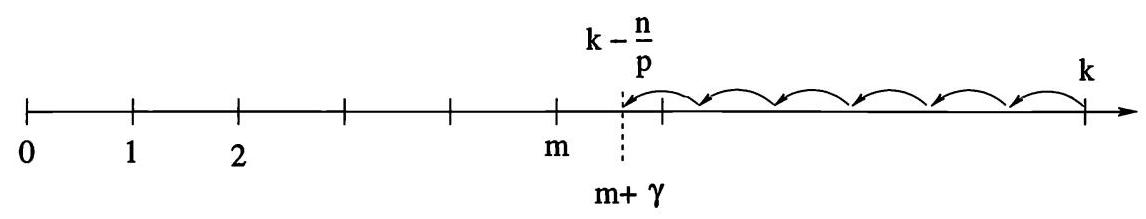
\includegraphics[width=1.0\textwidth]{images/bo_d6ik6nn7aajc739ct1l0_184_162_1681_1146_219_0.jpg}
\caption{计算函数 $f \in \; {W}^{k,p} \subset  {\mathcal{C}}^{m,\gamma }.$ 的“净光滑性”.}
\label{fig:net-smoothness}
\end{figure}

\begin{definition}{连续嵌入}
    称 Banach 空间 $X$ \colorbf{连续嵌入}于 Banach 空间 $Y$ ，若 $X \subseteq  Y$ ，且存在常数 $C$ ，使得
\[
\| u{\| }_{Y} \leq  C\| u{\| }_{X}\;\forall\,u \in  X.
\]
\end{definition}

\begin{theorem}[一般 Soblev 嵌入]\label{thm:sobolev-embedding-general}
设 $\Omega  \subset  {\mathbb{R}}^{n}$ 是具有 ${\mathcal{C}}^{1}$ 边界的有界开集，并考虑空间 ${W}^{k,p}\left( \Omega \right)$ .令 $m,\gamma$ 如\eqref{eq:net-smoothness}式所定义.则下列连续嵌入成立.
\begin{enumerate}[(i)]
    \item 若 $k - \frac{n}{p} < 0$ ，则 ${W}^{k,p}\left( \Omega \right)  \subseteq  {L}^{q}\left( \Omega \right)$ ，且 $\frac{1}{q} = \frac{1}{p} - \frac{k}{n} = \; \frac{1}{n}\left( {\frac{n}{p} - k}\right) .$
    \item 若 $k - \frac{n}{p} = 0$ ，则对每个 ${W}^{k,p}\left( \Omega \right)  \subseteq  {L}^{q}\left( \Omega \right)$ 有 $1 \leq  q < \infty$ .
    \item 若 $m \geq  0$ 且 $\gamma  > 0$ ，则 ${W}^{k,p}\left( \Omega \right)  \subseteq  {\mathcal{C}}^{m,\gamma }\left( \Omega \right)$ .
    \item 若 $m \geq  1$ 且 $\gamma  = 0$ ，则对每个 $0 \leq  {\gamma }^{\prime } < 1$ 有 ${W}^{k,p}\left( \Omega \right)  \subseteq  {\mathcal{C}}^{m - 1,{\gamma }^{\prime }}\left( \Omega \right)$ .
\end{enumerate}
\end{theorem}

\begin{remark}\label{rem:sobolev-embedding-meaning}
Soblev 空间中的函数仅在零测集意义下定义.我们说 ${W}^{k,p}\left( \Omega \right)  \subseteq  {\mathcal{C}}^{m,\gamma }\left( \Omega \right)$ ，意指如下:对每个 $u \in  {W}^{k,p}\left( \Omega \right)$ ，存在一个函数 $\widetilde{u} \in  {\mathcal{C}}^{m,\gamma }\left( \Omega \right)$ ，使得 $\widetilde{u}\left( x\right)  = \; u\left( x\right)$ 对几乎处处的 $x \in  \Omega$ 成立；此外，存在一个常数 $C$ ，它依赖于 $k,p,m,\gamma$ 但不依赖于 $u$ ，满足
\[
\| u{\| }_{{\mathcal{C}}^{m,\gamma }\left( \Omega \right) }\; \leq  \;C\| \widetilde{u}{\| }_{{W}^{k,p}\left( \Omega \right) }.
\]
\end{remark}

\begin{proof}
1．我们首先证明 (i)．假设 $k - \frac{n}{p} < 0$ ，并令 $u \in  {W}^{k,p}\left( \Omega \right)$ ．由于对每个 ${D}^{\alpha }u \in  {W}^{1,p}\left( \Omega \right)$ 有 $\left| \alpha \right|  \leq  k - 1$ ，Gagliardo-Nirenberg 不等式给出
\[
{\norm{D}^{\alpha }u}_{{L}^{{p}^{ * }}\left( \Omega \right) }\; \leq  C\norm{u}_{{W}^{k,p}\left( \Omega \right) },\;\left| \alpha \right|  \leq  k - 1\;.
\]

因此 $u \in  {W}^{k - 1,{p}^{ * }}\left( \Omega \right)$ ，其中 ${p}^{ * }$ 是 $p$ 的 Soblev 共轭指数.

该论证可迭代进行．令 ${p}_{1} = {p}^{ * },{p}_{2} \doteq  {p}_{1}^{ * },\ldots ,{p}_{j} \doteq  {p}_{j - 1}^{ * }$ ．由\eqref{eq:p-star-reciprocal}可知，当${jp} < n$时，
\[
\frac{1}{{p}_{1}} = \frac{1}{p} - \frac{1}{n},\;\ldots ,\;\frac{1}{{p}_{j}} = \frac{1}{p} - \frac{j}{n},
\]
多次应用 Gagliardo-Nirenberg 不等式，我们得到\eqref{eq:sobolev-iteration}
\begin{equation}\tag{8.70}\label{eq:sobolev-iteration}
{W}^{k,p}(\Omega )\; \subseteq  \;{W}^{k - 1,{p}_{1}}(\Omega )\; \subseteq  \;{W}^{k - 2,{p}_{2}}(\Omega )\; \subseteq  \;\cdots \; \subseteq  \;{W}^{k - j,{p}_{j}}(\Omega )\;.
\end{equation}
经过 $k$ 步后，我们得到 $u \in  {W}^{0,{p}_{k}}\left( \Omega \right)  = {L}^{{p}_{k}}\left( \Omega \right)$ ，其中 $\frac{1}{{p}_{k}} = \frac{1}{p} - \frac{k}{n} = \frac{1}{q}$ ．于是 ${p}_{k} = q$ ，(i) 得证.

\noindent 2．在特殊情形 ${kp} = n$ 下，重复上述论证，经过 $k - 1$ 步后我们得到
\[
\frac{1}{{p}_{k - 1}} = \frac{1}{p} - \frac{k - 1}{n} = \frac{1}{n}.
\]

因此 ${p}_{k - 1} = n$ ，且
\[
{W}^{k,p}\left( \Omega \right)  \subset  {W}^{1,n}\left( \Omega \right)  \subseteq  {W}^{1,n - \varepsilon }\left( \Omega \right)
\]
对每个 $\varepsilon  > 0$ 成立．再次应用 Gagliardo-Nirenberg 不等式，我们得到
\[
u \in  {W}^{1,n - \varepsilon }\left( \Omega \right)  \subseteq  {L}^{q}\left( \Omega \right) ,\;q = \frac{n\left( {n - \varepsilon }\right) }{n - \left( {n - \varepsilon }\right) } = \frac{{n}^{2} - {\varepsilon n}}{\varepsilon }.
\]

由于 $\varepsilon  > 0$ 是任意的，这就证明了 (ii).

\noindent 3．为证明 (iii)，假设 $m \geq  0$ 且 $\gamma  > 0$ ，并令 $u \in  {W}^{k,p}\left( \Omega \right)$ ．我们使用嵌入式\eqref{eq:sobolev-iteration}，选取 $j$ 为满足 ${p}_{j} > n$ 的最小整数．于是我们有
\[
\frac{1}{p} - \frac{j}{n} = \frac{1}{{p}_{j}} < \frac{1}{n} < \frac{1}{p} - \frac{j - 1}{n},\;u \in  {W}^{k - j,{p}_{j}}\left( \Omega \right) .
\]

因此，对任意满足 $\alpha$ 且 $\left| \alpha \right|  \leq  k - j - 1$ 的多重指标，Morrey 不等式给出
\[
{D}^{\alpha }u \in  {W}^{1,{p}_{j}}\left( \Omega \right)  \subseteq  {\mathcal{C}}^{0,\gamma }\left( \Omega \right) \;\text{其中}\;\gamma  = 1 - \frac{n}{{p}_{j}} = 1 - \frac{n}{p} + j.
\]

由于 $\alpha$ 是任一长度为 $\leq  k - j - 1$ 的多重指标，上述结论意味着
\[
u \in  {\mathcal{C}}^{k - j - 1,\gamma }\left( \Omega \right) \text{ . }
\]

为完成 (iii) 的证明，只需验证
\[
k - \frac{n}{p} = \left( {k - j - 1}\right)  + \left( {1 - \frac{n}{p} + j}\right) ,
\]

于是 $m = k - j - 1$ 为数 $k - \frac{n}{p}$ 的整数部分，而 $\gamma$ 为其小数部分.

\noindent 4. 为证明 (iv)，假设 $m \geq  1$ 且 $j \doteq  \frac{n}{p}$ 为整数.令 $u \in  {W}^{k,p}\left( \Omega \right)$ ，并任取满足 $\left| \alpha \right|  \leq  j - 1$ 的多重指标.仿照步骤 2 使用 Gagliardo-Nirenberg 不等式，可得
\[
{D}^{\alpha }u \in  {W}^{k - j,p}\left( \Omega \right)  \subseteq  {W}^{1,q}\left( \Omega \right)
\]
对每个 $1 < q < \infty$ 成立.故由 Morrey 不等式
\[
{D}^{\alpha }u \in  {W}^{1,q}\left( \Omega \right)  \subseteq  {\mathcal{C}}^{0,1 - \frac{n}{q}}\left( \Omega \right) .
\]

由于 $q$ 可任意大，这便证明了 (iv).
\end{proof}

\begin{instance}\label{ins:sobolev-embedding-example}
设 $\Omega$ 为 ${\mathbb{R}}^{5}$ 中的开单位球，并设 $u \in  {W}^{4,2}\left( \Omega \right)$ .连续两次应用 Gagliardo-Nirenberg 不等式，再应用 Morrey 不等式，可得
\[
u \in  {W}^{4,2}\left( \Omega \right)  \subset  {W}^{3,\frac{10}{3}}\left( \Omega \right)  \subset  {W}^{2,{10}}\left( \Omega \right)  \subset  {C}^{1,\frac{1}{2}}\left( \Omega \right) .
\]

注意， $u$ 的净光滑性为 $k - \frac{n}{p} = 4 - \frac{5}{2} = 1 + \frac{1}{2}.$
\end{instance}

\section{紧嵌入}

设 $\Omega  \subset  {\mathbb{R}}^{n}$ 为具有 ${\mathcal{C}}^{1}$ 边界的有界开集.本节将更深入地研究嵌入 ${W}^{1,p}\left( \Omega \right)  \subset  {L}^{q}\left( \Omega \right)$ ，并证明:当 $\frac{1}{q} > \frac{1}{p} - \frac{1}{n}$ 时，该嵌入是紧的.即，对任意在 ${W}^{1,p}$ 中有界的序列 ${\left( {u}_{m}\right) }_{m \geq  1}$ ，均可提取一个在 ${L}^{q}$ 中收敛的子列.

作为预备，我们注意到:若 $p > n$ ，则每个函数 $u \in \; {W}^{1,p}\left( \Omega \right)$ 均为 Hölder 连续.特别地，若 ${\left( {u}_{m}\right) }_{m \geq  1}$ 是 ${W}^{1,p}\left( \Omega \right)$ 中的有界序列，则函数族 ${u}_{m}$ 等度连续且一致有界.由 Arzelà-Ascoli 紧性定理，可提取子列 ${\left( {u}_{{m}_{j}}\right) }_{j \geq  1}$ ，其在 $\Omega$ 上一致收敛于某个连续函数 $u$ .由于 $\Omega$ 有界，这蕴含对每个 $q \in  \left(  {1,\infty }\right)$ 均有 ${\norm{u}_{{m}_{j}} - u}_{{L}^{q}\left( \Omega \right) } \rightarrow  0$ .这已表明:当 $p > n$ 且 $1 \leq  q \leq  \infty$ 时，嵌入 ${W}^{1,p}\left( \Omega \right)  \subset  {L}^{q}\left( \Omega \right)$ 是紧的.

因此，本节余下部分我们聚焦于情形 $p < n$ .由Gagliardo-Nirenberg不等式，空间 ${W}^{1,p}\left( \Omega \right)$ 连续嵌入于 ${L}^{{p}^{ * }}\left( \Omega \right)$ ，其中 ${p}^{ * } = \frac{np}{n - p}$ .进而，由于 $\Omega$ 有界，对每个 $1 \leq  q \leq  {p}^{ * }$ ，我们有连续嵌入 ${L}^{{p}^{ * }}\left( \Omega \right)  \subseteq  {L}^{q}\left( \Omega \right)$ .

\begin{theorem}[Rellich--Kondrachov紧性定理]\label{thm:rellich-kondrachov}
设 $\Omega  \subset  {\mathbb{R}}^{n}$ 为具有 ${\mathcal{C}}^{1}$ 边界的有界开集，且假设 $1 \leq  p < n$ .则对每个 $1 \leq  q < {p}^{ * } \doteq  \frac{np}{n - p}$ ，均有紧嵌入
\begin{equation}\tag{8.71}\label{eq:rellich-kondrachov}
{W}^{1,p}\left( \Omega \right)  \subset  \subset  {L}^{q}\left( \Omega \right) .
\end{equation}
\end{theorem}

\begin{proof}
1. 设 ${\left( {u}_{m}\right) }_{m \geq  1}$ 为 ${W}^{1,p}\left( \Omega \right)$ 中的有界序列.利用Soblev函数延拓定理\ref{thm:extension-operator}，可假设所有函数 ${u}_{m}$ 均定义在整个空间 ${\mathbb{R}}^{n}$ 上，且在某个紧集 $K$ 外恒为零:
\begin{equation}\tag{8.72}\label{eq:rellich-support}
\operatorname{Supp}\left( {u}_{m}\right)  \subseteq  K \subset  \widetilde{\Omega } \doteq  B\left( {\Omega ,1}\right) .
\end{equation}

此处右端表示围绕集合 $\Omega$ 的半径为一的开邻域.

由于 $q < {p}^{ * }$ 与 $\widetilde{\Omega }$ 有界，我们有
\[
{\norm{u}_{m}}_{{L}^{q}\left( {\mathbb{R}}^{n}\right) }  =  {\norm{u}_{m}}_{{L}^{q}\left( \widetilde{\Omega }\right) }  \leq   C {\norm{u}_{m}}_{{L}^{{p}^{ * }}\left( \widetilde{\Omega }\right) }  \leq   {C}^{\prime } {\norm{u}_{m}}_{{W}^{1,p}\left( \widetilde{\Omega }\right) }
\]

对某些常数 $C,{C}^{\prime }$ 成立.故序列 ${u}_{m}$ 在 ${L}^{q}\left( {\mathbb{R}}^{n}\right)$ 中一致有界.

\noindent 2. 考虑磨光函数 ${u}_{m}^{\varepsilon } \doteq  {J}_{\varepsilon } * {u}_{m}$ .由\eqref{eq:rellich-support}可知，所有这些函数均支撑于 $\widetilde{\Omega }$ 内.我们声称\eqref{eq:rellich-mollifier-conv}
\begin{equation}\tag{8.73}\label{eq:rellich-mollifier-conv}
{\norm{u_{m}^{\varepsilon } - {u}_{m}}}_{{L}^{q}\left( \widetilde{\Omega }\right) } \rightarrow  0,\;\;\varepsilon  \rightarrow  0,\;\text{关于}\;m\;\text{一致}.
\end{equation}

事实上，若 ${u}_{m}$ 光滑，则(作变量替换 ${y}^{\prime } = {\varepsilon y}$ 与 $z = x - {\varepsilon ty})$
{\setjot[-1]\begin{align*}
{u}_{m}^{\varepsilon }\left( x\right)  - {u}_{m}\left( x\right)  &= {\int }_{\left| {y}^{\prime }\right|  < \varepsilon }{J}_{\varepsilon }\left( {y}^{\prime }\right) \left(  {{u}_{m}\left( {x - {y}^{\prime }}\right)  - {u}_{m}\left( x\right) }\right)  d{y}^{\prime }\\
&= {\int }_{\left| y\right|  < 1}J\left( y\right) \left(  {{u}_{m}\left( {x - {\varepsilon y}}\right)  - {u}_{m}\left( x\right) }\right)  {\d y}\\
&= {\int }_{\left| y\right|  < 1}J\left( y\right) \left( {{\int }_{0}^{1}\frac{d}{\d t}\left( {{u}_{m}\left( {x - {\varepsilon ty}}\right) }\right) {\d t}}\right) {\d y}\\
&=  - \varepsilon {\int }_{\left| y\right|  < 1}J\left( y\right) \left( {{\int }_{0}^{1}\nabla {u}_{m}\left( {x - {\varepsilon ty}}\right)  \cdot  {y\d t}}\right) {\d y}.
\end{align*}}

进而得到
\begin{align*}
    \int_{\widetilde{\Omega }}\left| {u_m^{\varepsilon }(x)-u_m(x) }\right| {\d x} &\leq  \varepsilon {\int }_{\widetilde{\Omega }}{\int }_{\left| y\right| \leq  1}J\left( y\right) \left( {{\int }_{0}^{1}\left| {\nabla {u}_{m}\left( {x - {\varepsilon ty}}\right) }\right| {\d t}}\right) {\d y\d x}\\
    &\leq  \varepsilon {\int }_{\widetilde{\Omega }}\left| {\nabla {u}_{m}\left( z\right) }\right| {\d z}
\end{align*}


通过在 ${W}^{1,p}$ 中用光滑函数列逼近 ${u}_{m}$ ，可知该估计对所有函数 ${u}_{m} \in  {W}^{1,p}\left( \widetilde{\Omega }\right)$ 仍成立.因此我们已证得
\begin{equation}\tag{8.74}\label{eq:rellich-L1-estimate}
\norm{{u}_{m}^{\varepsilon }-{u}_{m}}_{{L}^{1}\left( \widetilde{\Omega }\right) }  \leq   \varepsilon \norm{\nabla {u}_{m}}_{{L}^{1}\left( \widetilde{\Omega }\right) }  \leq   {\varepsilon C}{\norm{u}_{m}}_{{W}^{1,p}\left( \widetilde{\Omega }\right) },
\end{equation}
对某个与 $m$ 无关的常数 $C$ 成立.由于范数 ${\norm{u}_{m}}_{{W}^{1,p}}$ 关于 $m$ 具有一致上界，这已证得我们在 $q = 1$ 情形下的断言\eqref{eq:rellich-mollifier-conv}.

\noindent 3. 为证 $1 < q < {p}^{ * }$ 情形下的\eqref{eq:rellich-mollifier-conv}，现使用 ${L}^{p}$ 范数的插值不等式(见附录(A.28)).选取 $0 < \theta  < 1$ 使得
\[
\frac{1}{q} = \theta  \cdot  1 + \left( {1 - \theta }\right)  \cdot  \frac{1}{{p}^{ * }}.
\]

则
\begin{equation}\tag{8.75}\label{eq:rellich-interpolation}
\| {u}_{m}^{\varepsilon } - {u}_{m} \|_{{L}^{q}\left( \widetilde{\Omega }\right) } \leq  \| {u}_{m}^{\varepsilon } - {u}_{m} \|_{{L}^{1}\left( \widetilde{\Omega }\right) }^{\theta } \cdot  \| {u}_{m}^{\varepsilon } - {u}_{m} \|_{{L}^{{p}^{ * }}\left( \widetilde{\Omega }\right) }^{1 - \theta } \leq  \left( {C}_{0}\varepsilon \right) ^{\theta }.
\end{equation}
对某个与 $m$ 无关的常数 ${C}_{0}$ 成立.事实上，在上述表达式中， ${L}^{1}$ 范数由\eqref{eq:rellich-L1-estimate}控制，而 ${L}^{{p}^{ * }}$ 范数则由定理\ref{thm:gagliardo-nirenberg}控制为某常数.

\noindent 4. 任取 $\delta  > 0$ ，并选取足够小的 $\varepsilon  > 0$ ，使得\eqref{eq:rellich-interpolation}给出
\[
{\norm{u}_{m}^{\varepsilon } - {u}_{m}}_{{L}^{q}\left( \widetilde{\Omega }\right) } \leq  {C}_{0}{\varepsilon }^{\theta } \leq  \frac{\delta }{2}\;\forall\,m \geq  1.
\]

回顾 ${u}_{m}^{\varepsilon } = {J}_{\varepsilon } * {u}_{m}$ ，我们有
{\begin{gather*}
    {\norm{u}_{m}^{\varepsilon }}_{{L}^{\infty }} \leq  {\norm{J}_{\varepsilon }}_{{L}^{\infty }}{\norm{u}_{m}}_{{L}^{1}} \leq  {C}_{1}\\
    \norm{\nabla {u}_{m}^{\varepsilon }}_{{L}^{\infty }} \leq  \norm{\nabla {J}_{\varepsilon }}_{{L}^{\infty }}{\norm{u}_{m}}_{{L}^{1}} \leq  {C}_{2}
\end{gather*}}
其中 ${C}_{1},{C}_{2}$ 是仅依赖于 $\varepsilon$ 而与 $m$ 无关的常数.上述不等式表明，对每个固定的 $\varepsilon  > 0$，序列 ${\left( {u}_{m}^{\varepsilon }\right) }_{m \geq  1}$ 一致有界且等度连续.由Ascoli紧性定理，存在子列 $\left( {u}_{{m}_{j}}^{\varepsilon }\right)$ 在 $\widetilde{\Omega }$ 上一致收敛于某个连续函数 ${u}^{\varepsilon }$ .我们现得到
\begin{equation}\tag{8.76}\label{eq:rellich-cauchy-estimate}
\begin{aligned}
\limsup_{{j,k \rightarrow  \infty }}\norm{{u}_{{m}_{j}} - {u}_{{m}_{k}}}_{{L}^{q}}
&\leq  \limsup_{{j,k \rightarrow  \infty }}\Bigl(
\norm{{u}_{{m}_{j}} - {u}_{{m}_{j}}^{\varepsilon }}_{{L}^{q}}
+ \norm{{u}_{{m}_{j}}^{\varepsilon } - {u}^{\varepsilon }}_{{L}^{q}} \\
&\quad +\norm{{u}^{\varepsilon } - {u}_{{m}_{k}}^{\varepsilon }}_{{L}^{q}}+\norm{{u}_{{m}_{k}}^{\varepsilon } - {u}_{{m}_{k}}}_{{L}^{q}}\Bigr) \\
&\leq  \frac{\delta }{2} + 0 + 0 + \frac{\delta }{2}.
\end{aligned}
\end{equation}

\noindent 5. 证明现通过标准对角化论证完成.由前一步可知，存在一个无穷指标集 ${I}_{1} \subset  \mathbb{N}$ ，使得子列 ${\left( {u}_{m}\right) }_{m \in  {I}_{1}}$ 满足
\[
\limsup_{{\ell ,m \rightarrow  \infty ,\ell ,m \in  {I}_{1}}}{\norm{u}_{\ell } - {u}_{m}}_{{L}^{q}} \leq  {2}^{-1}
\]

对 $j = 1,2,\ldots$ 归纳:在 ${I}_{j - 1}$ 构造完成后，选取一个无穷指标集 ${I}_{j} \subset  {I}_{j - 1} \subset  \mathbb{N}$ ，使得子列 ${\left( {u}_{m}\right) }_{m \in  {I}_{j}}$ 满足
\[
\limsup_{{\ell ,m \rightarrow  \infty ,\ell ,m \in  {I}_{j}}}{\norm{u}_{\ell } - {u}_{m}}_{{L}^{q}} \leq  {2}^{-j}
\]

在对所有 $j \geq  1$ 构造完子集 ${I}_{j}$ 后，再对 $j$ 归纳，选取一列整数 ${m}_{1} < {m}_{2} < {m}_{3} < \cdots$ ，使得对每个 $j$ 均有 ${m}_{j} \in  {I}_{j}$ .该子列 ${\left( {u}_{{m}_{j}}\right) }_{j \geq  1}$ 满足
\[
\limsup_{{j,k \rightarrow  \infty }}{\norm{u}_{{m}_{j}} - {u}_{{m}_{k}}}_{{L}^{q}} = 0.
\]

因此该子列是Cauchy列，收敛于某个极限 $u \in  {L}^{q}$ .这证明了当 $p < n$ 时嵌入\eqref{eq:rellich-kondrachov}是紧的.
\end{proof}

\begin{corollary}\label{cor:H1-L2-compact-embedding}
设 $\Omega  \subset  {\mathbb{R}}^{n}$ 是具有 ${\mathcal{C}}^{1}$ 边界的有界开集，则有如下紧嵌入
\[
{H}^{1}\left( \Omega \right)  \subset  \subset  {L}^{2}\left( \Omega \right) .
\]
\end{corollary}

\begin{proof}
当 $n > 2$ 时，结论是定理\ref{thm:rellich-kondrachov}(取 $p = 2$ )的特例；当 $n = 1$ 时， ${H}^{1}\left( \Omega \right)$ 中每个函数均为Hölder连续，结果由 Ascoli 定理得出；当 $n = 2$ 时，可对 $p = 3/2,{p}^{ * } = 6,q = 2$ 应用定理\ref{thm:rellich-kondrachov}，得到
\[
{W}^{1,2}\left( \Omega \right)  \subset  {W}^{1,3/2}\left( \Omega \right)  \subset  \subset  {L}^{2}\left( \Omega \right) .
\]
\end{proof}

作为紧嵌入定理的一个应用，我们现证明函数 $u$ 与其在区域 $\Omega$ 上平均值之差的一个估计.

\begin{theorem}[Poincar\'e不等式 II]\label{thm:poincare-inequality-ii}
设 $\Omega  \subset  {\mathbb{R}}^{n}$ 是具有 ${\mathcal{C}}^{1}$ 边界的有界连通开集，且设 $p \in  \left(  {1,\infty }\right)$ .则存在仅依赖于 $p$ 和 $\Omega$ 的常数 $C$ ，使得
\begin{equation}\tag{8.77}\label{eq:poincare-ii}
\norm{u - {\int }_{\Omega }u\,\d x}_{{L}^{p}\left( \Omega \right) }\; \leq  \;C\norm{\nabla u}_{{L}^{p}\left( \Omega \right) }.
\end{equation}

对每个 $u \in  {W}^{1,p}\left( \Omega \right)$ 成立.
\end{theorem}

\begin{proof}
若结论不成立，则可找到一列函数 ${u}_{k} \in  {W}^{1,p}\left( \Omega \right)$ ，满足
\[
\norm{{u}_{k} - {\int }_{\Omega }{u}_{k}\,\d x}_{{L}^{p}\left( \Omega \right) } > k\norm{\nabla {u}_{k}}_{{L}^{p}\left( \Omega \right) }
\]

对每个 $k = 1,2,\ldots$ 成立.于是归一化函数
\[
{v}_{k} \doteq  \frac{{u}_{k} - {\int }_{\Omega }{u}_{k}\,\d x}{\norm{{u}_{k} - {\int }_{\Omega }{u}_{k}\,\d x}_{{L}^{p}\left( \Omega \right) }}
\]
满足
\begin{equation}\tag{8.78}\label{eq:poincare-ii-normalization}
{\int }_{\Omega }{v}_{k}\,\d x = 0,\;{\norm{v}_{k}}_{{L}^{p}\left( \Omega \right) } = 1,\;{\norm{\nabla {v}_{k}}}_{{L}^{p}\left( \Omega \right) } < \frac{1}{k},\;k = 1,2,\ldots
\end{equation}

由于序列 ${\left( {v}_{k}\right) }_{k \geq  1}$ 在 ${W}^{1,p}\left( \Omega \right)$ 中有界，若 $p < n$ ，则可应用定理\ref{thm:rellich-kondrachov}(取 $q = p$ )，找到一个在 ${L}^{p}\left( \Omega \right)$ 中收敛于某个函数 $v$ 的子列.若 $p > n$ ，则由\eqref{eq:morrey-embedding}可知函数 ${v}_{k}$ 一致有界且 Hölder 连续.于是利用 Ascoli 紧性定理，可找到一个在 $\Omega$ 上一致收敛于某个连续函数 $v$ 的子列，从而也在 ${L}^{p}\left( \Omega \right)$ 中收敛于 $v$.

由\eqref{eq:poincare-ii-normalization}，弱梯度序列亦收敛，即 $\nabla {v}_{k} \to 0$ 于 ${L}^{p}\left( \Omega \right)$ 中.由引理 8.14，零函数是极限函数 $v$ 的弱梯度.

我们现已有
\[
{\int }_{\Omega }v\,\d x = \mathop{\lim }\limits_{{k \rightarrow  \infty }}{\int }_{\Omega }{v}_{k}\,\d x = 0.
\]
此外，由于 $\nabla v = 0 \in  {L}^{p}\left( \Omega \right)$ ，由推论 8.16 可知函数 $v$ 在连通集 $\Omega$ 上必为常数；结合 $\int_{\Omega } v\,\d x = 0$ ，可得 $v = 0$ 几乎处处成立.

另一方面，由 ${v}_{k} \to v$ 于 ${L}^{p}\left( \Omega \right)$ 及\eqref{eq:poincare-ii-normalization}可得 $\norm{v}_{{L}^{p}\left( \Omega \right) } = 1$ ，矛盾.
\end{proof}

\section{可微性性质}

由 Morrey 不等式，若 $\Omega  \subset  {\mathbb{R}}^{n}$ 且 $w \in  {W}^{1,p}\left( \Omega \right)$ 满足 $p > n$ ，则 $w$ 几乎处处等于一个 Hölder 连续函数.事实上，在零测集上适当修改后，我们有
\begin{equation}\tag{8.79}\label{eq:morrey-pointwise}
\left| {w\left( x\right)  - w\left( y\right) }\right|  \leq  C{\left| x - y\right| }^{1 - \frac{n}{p}}{\left( {\int }_{B\left( {x,\left| {y - x}\right| }\right) }{\left| \nabla w\left( z\right) \right| }^{p}\d z\right) }^{1/p}.
\end{equation}

仅此本身并不意味着 $u$ 必须在经典意义下可微.事实上，存在处处不可微的 Hölder 连续函数.然而，对 Soblev 空间中的函数，可证明更强的正则性结果.

\begin{theorem}[几乎处处可微性]\label{thm:a-e-differentiability}
设 $\Omega  \subseteq  {\mathbb{R}}^{n}$ ，且对某个 $p > n$ 有 $u \in  {W}_{\text{ loc }}^{1,p}\left( \Omega \right)$ .则 $u$ 在几乎处处的点 $x \in  \Omega$ 可微，且其梯度与弱梯度重合.
\end{theorem}

\begin{proof}
令 $u \in  {W}_{\text{ loc }}^{1,p}\left( \Omega \right)$ .由于弱导数属于 ${L}_{\text{ loc }}^{p}$ ，弱梯度 $\nabla u \doteq  \left( {{D}_{{x}_{1}}u,\ldots ,{D}_{{x}_{n}}u}\right)$ 同样属于 ${L}_{\text{ loc }}^{p}$ .由 Lebesgue 微分定理，对几乎处处的 $x \in  \Omega$ ，有
\begin{equation}\tag{8.80}\label{eq:lebesgue-diff-grad}
{\oint }_{B\left( {x,r}\right) }{\left| \nabla u\left( x\right)  - \nabla u\left( z\right) \right| }^{p}{\d z} \rightarrow  0\;\text{ as }r \rightarrow  0.
\end{equation}

固定一个满足\eqref{eq:lebesgue-diff-grad}的点 $x$ ，并定义
\begin{equation}\tag{8.81}\label{eq:def-w-for-diff}
w\left( y\right)  \doteq  u\left( y\right)  - u\left( x\right)  - \nabla u\left( x\right)  \cdot  \left( {y - x}\right) .
\end{equation}

注意到 $w \in  {W}_{\text{ loc }}^{1,p}\left( \Omega \right)$ ，可应用估计式\eqref{eq:morrey-pointwise}，得

{\begin{align*}
    \left| {w\left( y\right)  - w\left( x\right) }\right|  &= \left| {w\left( y\right) }\right|  = \left| {u\left( y\right)  - u\left( x\right)  - \nabla u\left( x\right)  \cdot  \left( {y - x}\right) }\right|\\
    &\leq  C{\left| y - x\right| }^{1 - \frac{n}{p}}{\left( {\int }_{B\left( {x,\left| {y - x}\right| }\right) }{\left| \nabla u\left( x\right)  - \nabla u\left( z\right) \right| }^{p}\d z\right) }^{1/p}\\
    &\leq  {C}^{\prime }\left| {y - x}\right| {\left( {f}_{B\left( {x,\left| {y - x}\right| }\right) }{\left| \nabla u\left( x\right)  - \nabla u\left( z\right) \right| }^{p}\d z\right) }^{1/p}
\end{align*}}
对某些常数 $C,{C}^{\prime }$ 成立.因此
\[
\frac{\left| w\left( y\right)  - w\left( x\right) \right| }{\left| y - x\right| } \rightarrow  0\;\text{ as }\left| {y - x}\right|  \rightarrow  0.
\]

由\eqref{eq:def-w-for-diff}中 $w$ 的定义可知， $u$ 在 $x$ 处经典可微，且其梯度与弱梯度重合.
\end{proof}

\section{习题}

\begin{rbhw}[index=1]
判定下列泛函中哪些在 $\Omega  \subseteq  \mathbb{R}$ 上定义了一个分布.
\begin{enumerate}[(i)]
    \item $\Lambda \left( \phi \right)  = \sum_{{k = 1}}^{\infty }k!{D}^{k}\phi \left( k\right)$ ，其中 $\Omega  = \mathbb{R}$ .
    \item $\Lambda \left( \phi \right)  = \sum_{{k = 1}}^{\infty }{2}^{-k}{D}^{k}\phi \left( {1/k}\right)$ ，且 $\Omega  = \mathbb{R}$ .
    \item $\Lambda \left( \phi \right)  = \sum_{{k = 1}}^{\infty }\frac{\phi \left( {1/k}\right) }{k}$ ，且 $\Omega  = \mathbb{R}$ .
    \item $\Lambda \left( \phi \right)  = {\int }_{0}^{\infty }\frac{\phi \left( x\right) }{{x}^{2}}\,\d x$ ，且 $\Omega = (0,\infty)$ .
\end{enumerate}
\end{rbhw}

\begin{rbhw}
给出直接证明:若对某个 $f \in  {W}^{1,p}(a,b)$ 、 $a < b$ 和 $1 < p < \infty$ ，则通过在零测集上修改 $f$ ，可得
\[
\left| {f\left( x\right)  - f\left( y\right) }\right|  \leq  C{\left| x - y\right| }^{1 - \frac{1}{p}}\;\forall\,x,y \in  ( a,b) .
\]
计算最优常数 $C$ .
\end{rbhw}

\begin{rbhw}
考虑开正方形
\[
Q \doteq  \left\{  {\left( {{x}_{1},{x}_{2}}\right) ;0 < {x}_{1} < 1,0 < {x}_{2} < 1}\right\}   \subset  {\mathbb{R}}^{2}.
\]

设 $f \in  {W}^{1,1}\left( Q\right)$ 为一函数，其弱导数满足对几乎处处 $x \in  Q$ 有 ${D}_{{x}_{1}}f\left( x\right)  = 0$ .证明存在一函数 $g \in  {L}^{1}\left( \left(  {0,1}\right)  \right)$ ，使得
\[
f\left( {{x}_{1},{x}_{2}}\right)  = g\left( {x}_{2}\right) \;\text{ for a.e. }\left( {{x}_{1},{x}_{2}}\right)  \in  Q.
\]
\end{rbhw}

\begin{rbhw}
设 $\Omega  \subseteq  {\mathbb{R}}^{n}$ 为开集，且假设 $f \in  {L}_{\text{ loc }}^{1}\left( \Omega \right)$ .设 $g = {D}_{{x}_{1}}f$ 为 $f$ 关于 ${x}_{1}$ 的弱导数.若 $f$ 在开子集 ${\Omega }^{\prime } \subseteq  \Omega$ 上等于 ${\mathcal{C}}^{1}$ ，则证明 $g$ 在几乎处处点 $x \in  {\Omega }^{\prime }$ 上与偏导数 $\partial f/\partial {x}_{1}$ 重合.
\end{rbhw}

\begin{rbhw}
(i) 证明:若对某个开凸集 $\Omega  \subseteq  {\mathbb{R}}^{n}$ 有 $u \in  {W}^{1,\infty }\left( \Omega \right)$ ，则 $u$ 几乎处处与一个Lipschitz连续函数重合.

(ii) 证明:存在一个(非凸的)连通开集 $\Omega  \subset  {\mathbb{R}}^{n}$ 及一个函数 $u \in  {W}^{1,\infty }\left( \Omega \right)$ ，其不与任何Lipschitz连续函数几乎处处重合.
\end{rbhw}

\begin{rbhw}
(Rademacher定理)设 $\Omega  \subset  {\mathbb{R}}^{n}$ 为开集， $u : \Omega  \mapsto  \mathbb{R}$ 为有界Lipschitz连续函数.
\begin{enumerate}[(i)]
    \item 证明: $u \in  {W}^{1,\infty }\left( \Omega \right)$ .
    \item 证明: $u$ 在几乎处处点 $x \in  \Omega$ 上可微.
\end{enumerate}
\textcolor{gray}{(i) 的提示:先考虑 $\Omega$ 为凸集的情形.为构造弱导数 ${D}_{{x}_{i}}$ ，对任意固定 ${x}_{1},\ldots ,{x}_{i - 1},{x}_{i + 1},\allowbreak \ldots ,{x}_{n}$，考虑绝对连续函数 $s \mapsto  u( {x}_{1},\ldots ,{x}_{i - 1},s,{x}_{i + 1},\ldots ,{x}_{n} )$ .}
\end{rbhw}

\begin{rbhw}
设 $\Omega  = B\left( {0,1}\right)$ 为 ${\mathbb{R}}^{n}$ 中的开单位球，其中 $n \geq  2$ .证明无界函数 $f\left( x\right)  = \ln \ln \left( {1 + \frac{1}{\left| x\right| }}\right)$ 属于 ${W}^{1,n}\left( \Omega \right)$ .
\end{rbhw}

\begin{rbhw}
(i) 设 $\Omega  = (-1,1)$ .考虑由 ${Tf} = f\left( 0\right)$ 定义的线性映射 $T : {\mathcal{C}}^{1}\left( \Omega \right)  \mapsto  \mathbb{R}$ .证明该映射可唯一连续延拓为一个有界线性泛函 $T : {W}^{1,1}\left( \Omega \right)  \mapsto  \mathbb{R}$ .\par
\indent (ii) 设 $\Omega  = B\left( {0,1}\right)  \subset  {\mathbb{R}}^{2}$ 为开单位圆盘.再次考虑由 ${Tf} = f\left( 0\right)$ 定义的线性映射 $T : {\mathcal{C}}^{1}\left( \Omega \right)  \mapsto  \mathbb{R}$ .对该映射，当 $p$ 取何值时，它可连续延拓为一个有界线性泛函 $T : {W}^{1,p}\left( \Omega \right)  \mapsto  \mathbb{R}$ ？
\end{rbhw}

\begin{rbhw}
确定对哪些 $p \geq  1$ 值，一般函数 $f \in  {W}^{1,p}\left( {\mathbb{R}}^{3}\right)$ 沿 ${x}_{1}$ -轴存在迹.换言之，令 $\Gamma  \doteq  \{ \left( {t,0,0}\right) ;t \in  \mathbb{R}\}  \subset  {\mathbb{R}}^{3}$ ，并考虑映射 $T : {\mathcal{C}}_{\mathrm{c}}^{1}\left( {\mathbb{R}}^{3}\right)  \mapsto  {L}^{p}\left( \Gamma \right)$ ，其中 ${Tf} = {f}_{\mid \Gamma }$ 是 $f$ 在 $\Gamma$ 上的限制.求使该映射存在连续延拓 $T : {W}^{1,p}\left( {\mathbb{R}}^{3}\right)  \mapsto  {L}^{p}\left( \Gamma \right)$ 的 $p$ 值.
\end{rbhw}

\begin{rbhw}
设 $V \subset  {\mathbb{R}}^{n}$ 是维数为 $m$ 的子空间， ${V}^{ \bot  }$ 是其正交补子空间，维数为 $n - m$ .设 $u \in  {W}^{1,p}\left( {\mathbb{R}}^{n}\right)$ 且 $m < p < n$ .证明:在零测集上适当修改后，以下结论成立.
\begin{enumerate}[(i)]
    \item 对几乎处处的 $y \in  {V}^{ \bot  }$ (关于 $\left( {n - m}\right)$ -维测度)， $u$ 在仿射子空间 $y + V$ 上的限制是指数为 $\gamma  = 1 - \frac{m}{p}$ 的 Hölder 连续函数.
    \item 点态值 $u\left( y\right)$ 对几乎处处的 $y \in  {V}^{ \bot  }$ 有定义.此外
\[
\| u\left( y\right) {\| }_{{L}^{p}\left( {V}^{ \bot  }\right) } \leq  C \cdot  \| u{\| }_{{W}^{1,p}\left( {\mathbb{R}}^{n}\right) }
\]
其中常数 $C$ 依赖于 $m,n,p$ ，但与 $u$ 无关.
\end{enumerate}
\end{rbhw}

\begin{rbhw}
设 $\Omega  \subset  {\mathbb{R}}^{n}$ 为任意开集(不假设边界具有任何正则性)，并设 $p > n$ .证明:每个函数 $f \in  {W}_{0}^{1,p}\left( \Omega \right)$ 几乎处处等于某个连续函数 $\widetilde{f}$ .此外，存在一个常数 $C$ ，其仅依赖于 $p,n$ ，而与 $\Omega$ 或 $f$ 无关，使得
\[
\| \widetilde{f}{\| }_{{\mathcal{C}}^{0,\gamma }\left( \Omega \right) } \leq  C\| f{\| }_{{W}^{1,p}\left( \Omega \right) }\;\text{ with }\gamma  = 1 - \frac{n}{p}.
\]
\end{rbhw}

\begin{rbhw}
当 $k = 0$ 时，依定义有 ${W}^{0,p}\left( \Omega \right)  = {L}^{p}\left( \Omega \right)$ .若 $1 \leq  p < \infty$ ，则证明 ${W}_{0}^{0,p}\left( \Omega \right)  = {L}^{p}\left( \Omega \right)$ 亦成立. ${W}_{0}^{0,\infty }\left( \Omega \right)$ 是什么？
\end{rbhw}

\begin{rbhw}
设 $\varphi  : \mathbb{R} \mapsto  \left(  {0,1}\right)$ 为一光滑函数，满足
\[
\varphi \left( r\right)  =\begin{cases} 1 & \text{ if }r \leq  0, \\  0 & \text{ if }r \geq  1. \end{cases}
\]
对任意 $f \in  {W}^{k,p}\left( {\mathbb{R}}^{n}\right)$ ，证明函数 ${f}_{k}\left( x\right)  = f\left( x\right) \varphi \left( {\left| x\right|  - k}\right)$ 在 ${W}^{k,p}\left( {\mathbb{R}}^{n}\right)$ 中收敛于 $f$，对每个 $k \geq  0$ 和 $1 \leq  p < \infty$ 均成立.由此推出， ${W}_{0}^{k,p}\left( {\mathbb{R}}^{n}\right)  = {W}^{k,p}\left( {\mathbb{R}}^{n}\right) .$
\end{rbhw}

\begin{rbhw}
设 ${\mathbb{R}}_{ + } \doteq  \{ x \in  \mathbb{R};x > 0\}$ ，并假设 $u \in  {W}^{2,p}\left( {\mathbb{R}}_{ + }\right)$ .通过定义 $u$ 的对称延拓: ${Eu}\left( x\right)  \doteq  u\left( \left| x\right| \right)$ .证明 ${Eu} \in  {W}^{1,p}\left( \mathbb{R}\right)$ ，但一般地 ${Eu} \notin \; {W}^{2,p}\left( \mathbb{R}\right)$ .
\end{rbhw}

\begin{rbhw}
设 $u \in  {\mathcal{C}}_{c}^{1}\left( {\mathbb{R}}^{n}\right)$ ，并固定 $p,q \in  (1,\infty)$ .对给定的 $\lambda  > 0$ ，考虑其缩放函数 ${u}_{\lambda }\left( x\right)  \doteq  u\left( {\lambda x}\right)$ .
\begin{enumerate}[(i)]
    \item 证明存在一个依赖于 $n,q$ 的指数 $\alpha$ ，使得
\[
{\norm{u}_{\lambda }}_{{L}^{q}\left( {\mathbb{R}}^{n}\right) } = {\lambda }^{\alpha }\| u{\| }_{{L}^{q}\left( {\mathbb{R}}^{n}\right) }.
\]
    \item 证明存在一个依赖于 $n,p$ 的指数 $\beta$ ，使得
\[
\| \nabla {u}_{\lambda }{\| }_{{L}^{p}\left( {\mathbb{R}}^{n}\right) } = {\lambda }^{\beta }\| \nabla u{\| }_{{L}^{p}\left( {\mathbb{R}}^{n}\right) }.
\]
    \item  确定使 $\alpha  = \beta$ 成立的 $n,p,q$ 的取值范围，并与\eqref{eq:p-star}比较.
\end{enumerate}
\end{rbhw}

\begin{rbhw}
设 $\Omega  \subset  {\mathbb{R}}^{n}$ 是具有 ${\mathcal{C}}^{1}$ 边界的有界开集， ${\left( {u}_{m}\right) }_{m \geq  1}$ 是一列在 ${H}^{1}\left( \Omega \right)$ 中一致有界的函数.若假设 ${\norm{u}_{m} - u}_{{L}^{2}} \rightarrow  0$ ，则证明 $u \in  {H}^{1}\left( \Omega \right)$ ，且
\[
\| u{\| }_{{H}^{1}} \leq  \mathop{\liminf }\limits_{{m \rightarrow  \infty }}{\norm{u}_{m}}_{{H}^{1}}.
\]
\end{rbhw}

\begin{rbhw}
设 $\Omega  \doteq  \left\{  {\left( {{x}_{1},{x}_{2}}\right) ;{x}_{1}^{2} + {x}_{2}^{2} < 1}\right\}$ 为 ${\mathbb{R}}^{2}$ 中的开单位圆盘， ${\Omega }_{0} \doteq  \Omega  \setminus  \{ \left( {0,0}\right) \}$ 为去掉原点的单位圆盘.考虑函数 $f\left( x\right)  \doteq  1 - \left| x\right|$ .证明(见图\ref{fig:exercise-17})
\begin{enumerate}[(i)]
    \item  若$1 \leq  p < \infty$，则$f  \in  {W}_{0}^{1,p}\left( \Omega \right)$.
    \item 若$1 \leq  p \leq  2$，则$f  \in  {W}_{0}^{1,p}\left( {\Omega }_{0}\right)$；
    \item 若$2 < p \leq  \infty$，则$f  \notin  {W}_{0}^{1,p}\left( \Omega \right)$.
\end{enumerate}
\begin{figure}[htbp]
\centering
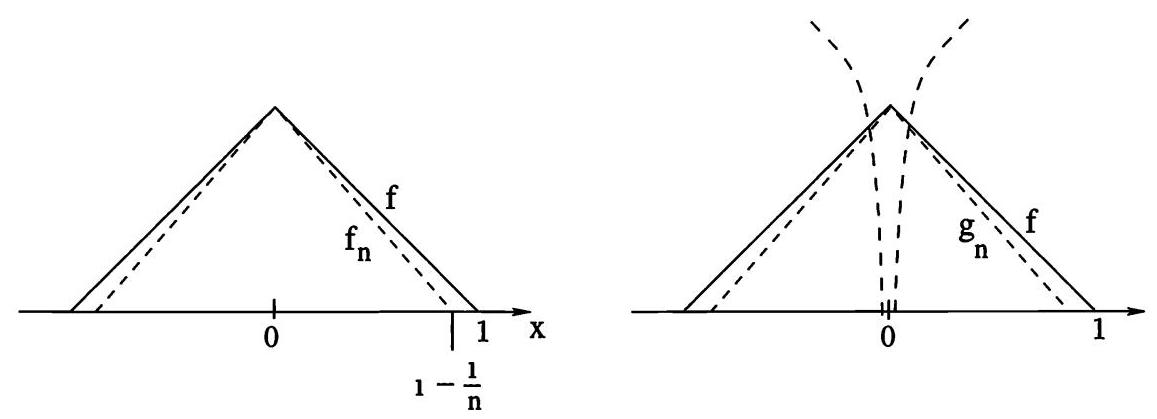
\includegraphics[width=1.0\textwidth]{images/bo_d6ik6nn7aajc739ct1l0_195_164_238_1157_419_0.jpg}
\caption{左:函数 $f$ 可在 ${W}^{1,p}$ 中用支集位于 $\Omega$ 内的函数 ${f}_{n}$ 逼近；右:函数 $f$ 可在 ${W}^{1,2}$ 中用支集位于 ${\Omega }_{0}$ 内的函数 ${g}_{n}$ 逼近.}
\label{fig:exercise-17}
\end{figure}
\end{rbhw}

\begin{rbhw}
设 $\Omega  = \left\{  {\left( {{x}_{1},{x}_{2}}\right) ;0 < {x}_{1} < 1,0 < {x}_{2} < 1}\right\}$ 为 ${\mathbb{R}}^{2}$ 中的开单位正方形.
\begin{enumerate}[(i)]
    \item 若 $u \in  {H}^{1}\left( \Omega \right)$ 满足
\[
\operatorname{meas}\left( {\{ x \in  \Omega ;u\left( x\right)  = 0\} }\right)  > 0,\;\nabla u\left( x\right)  = 0\text{ for a.e. }x \in  \Omega ,
\]
证明:对几乎处处的 $x \in  \Omega$ ，有 $u\left( x\right)  = 0$ .
    \item 对每个 $\alpha  > 0$ ，证明存在常数 ${C}_{\alpha }$ ，满足如下性质:若函数 $u \in  {H}^{1}\left( \Omega \right)$ 满足 $\operatorname{meas}\left( \{x \in \Omega ; u\left( x\right) = 0\}\right) \geq \alpha$ ，则
\begin{equation}\tag{8.82}\label{eq:exercise-18-poincare}
\| u{\| }_{{L}^{2}\left( \Omega \right) } \leq  {C}_{\alpha }\| \nabla u{\| }_{{L}^{2}\left( \Omega \right) }.
\end{equation}
\end{enumerate}
\end{rbhw}

\begin{rbhw}
设 $\Omega  \subseteq  {\mathbb{R}}^{n}$ 为开集， $K \subset  \Omega$ 为“小”的闭集，即其 $\left( {n - 1}\right)$ 维测度为 ${m}_{n - 1}\left( K\right)  = 0$.更准确地说，假设 $K$ 在任意 $\left( {n - 1}\right)$ 维超平面上的投影具有零 $\left( {n - 1}\right)$ 维测度.设 $u$ 在开集 $\Omega  \backslash  K$ 上连续可微，且满足 $u \in  {L}^{p}\left( {\Omega  \backslash  K}\right) ,\nabla u \in  {L}^{p}\left( {\Omega  \backslash  K}\right)$ .证明: $u \in  {W}^{1,p}\left( \Omega \right)$.
\end{rbhw}

\begin{rbhw}
(i) 找出两个函数 $f,g \in  {L}_{\text{ loc }}^{1}\left( {\mathbb{R}}^{n}\right)$ ，使得其乘积 $f \cdot  g$ 不是局部可和的.
(ii) 证明:若 $f,g \in  {L}_{\text{ loc }}^{1}\left( \mathbb{R}\right)$ 均有界且弱可微，则其乘积 $f \cdot  g$ 也弱可微，并满足通常的乘积法则: ${D}_{x}\left( {fg}\right)  = \left( {{D}_{x}f}\right)  \cdot  g + f \cdot  \left( {{D}_{x}g}\right)$ .
(iii) 找出两个函数 $f,g \in  {L}_{\text{ loc }}^{1}\left( {\mathbb{R}}^{n}\right)$ (其中 $n \geq  2$ )，满足如下性质:对任意 $i = 1,\ldots ,n$ ，一阶弱导数 ${D}_{{x}_{i}}f,{D}_{{x}_{i}}g$ 均有定义；但乘积 $f \cdot  g$ 在整个空间 ${\mathbb{R}}^{n}$ 上无任何弱导数.
\end{rbhw}

\begin{rbhw}
设 $\Omega  \subset  {\mathbb{R}}^{n}$ 为具有 ${\mathcal{C}}^{1}$ 边界的有界连通开集， ${\Omega }^{\prime } \subset  \Omega$ 为非空开子集，且 $p \in  \left(  {1,\infty }\right)$.证明:存在常数 $C$ ，使得
\[
\norm{u}_{{L}^{p}\left( \Omega \right) }\; \leq  \;C\left( {\| u{\| }_{{L}^{p}\left( {\Omega }^{\prime }\right) } + \| \nabla u{\| }_{{L}^{p}\left( \Omega \right) }}\right) \;\text{ for every }u \in  {W}^{1,p}\left( \Omega \right) \;.
\]
\end{rbhw}

\begin{rbhw}
考虑开区间 $(0,1)$配备范数$\|f\|_{{\mathcal{C}}^{0}} = \sup_{{0 < x < 1}}{\left| {f\left( x\right) }\right|}$ 上所有有界连续函数构成的 Banach 空间 $X = {C}^{0}\left( {( 0,1) }\right)$ .对固定常数 $M > 0$ ，令 ${S}_{M} \subset  X$ 为满足 $\| f{\| }_{{W}^{2,\infty }} \leq  M$ 的所有函数 $f \in  X$ 构成的子集.换言之， $f \in  {S}_{M}$ 当且仅当 $f$ 具有直至二阶的弱导数，且
\[
\| f{\| }_{{L}^{\infty }} \leq  M,\;\| {\partial }_{x}f{\| }_{{L}^{\infty }} \leq  M,\;\| {\partial }_{xx}f{\| }_{{L}^{\infty }} \leq  M.
\]
\begin{enumerate}[(i)]
    \item 证明 ${S}_{M}$ 是 $X$ 的闭子集.
    \item 证明微分算子 $f \mapsto  {\partial }_{x}f$ 在集合 ${S}_{M}$ 上的限制是连续的.换言之，若 ${\norm{f}_{n} - f}_{{\mathcal{C}}^{0}} \rightarrow  0$ 且对所有 $n \geq  1$ 有 $f,{f}_{n} \in  {S}_{M}$ ，则 ${\norm{\partial }_{x}{f}_{n} - {\partial }_{x}f}_{{\mathcal{C}}^{0}} \rightarrow  0$ .
\end{enumerate}
\end{rbhw}

\begin{rbhw}
设 $\Omega  \subset  {\mathbb{R}}^{n}$ 是一个具有 ${\mathcal{C}}^{1}$ 边界的有界开集.对任意满足 $1 \leq  p < \infty$ 的 $u \in  {W}^{1,p}\left( \Omega \right)$ ，证明存在一列光滑函数 ${u}_{k} \in \; {\mathcal{C}}_{c}^{\infty }\left( {\mathbb{R}}^{n}\right)$ ，使得 ${u}_{k}$ 在 $\Omega$ 上的限制满足
\[
\mathop{\lim }\limits_{{k \rightarrow  \infty }}\| {u}_{k} - u{\| }_{{W}^{1,p}\left( \Omega \right) } = 0.
\]

此外，
\[
{\norm{u}_{k}}_{{W}^{1,p}\left( {\mathbb{R}}^{n}\right) } \leq  C\| u{\| }_{{W}^{1,p}\left( \Omega \right) },
\]
其中常数 $C$ 仅依赖于 $p$ 和 $\Omega$ ，而与 $u$ 无关.
\end{rbhw}

\begin{rbhw}
设 $f : \mathbb{R} \mapsto  \mathbb{R}$ 是一个弱可微函数，其弱导数为 $g \in \; {L}_{\text{ loc }}^{1}\left( \mathbb{R}\right)$ .考虑差商序列 ${g}_{n}\left( x\right)  = n\left(  {f\left( {x + \frac{1}{n}}\right)  - f\left( x\right) }\right)$ .证明:对几乎处处的 $x \in  \mathbb{R}$ ，有 ${g}_{n}\left( x\right)  \rightarrow  g\left( x\right)$ ；且对任意有界区间 $\left(  {a,b}\right)$ ，均有 ${\norm{g}_{n} - g}_{{L}^{1}\left( \left(  {a,b}\right)  \right) } \rightarrow  0$ .
\end{rbhw}

\begin{rbhw}
设 ${\left( {u}_{n}\right) }_{n \geq  1}$ 是 Hilbert 空间 ${H}^{2}\left( {\mathbb{R}}^{3}\right)  \doteq  {W}^{2,2}\left( {\mathbb{R}}^{3}\right)$ 中的一列函数.假设
\[
\mathop{\lim }\limits_{{n \rightarrow  \infty }}{u}_{n}\left( x\right)  = u\left( x\right) \;\forall\,x \in  {\mathbb{R}}^{3},\;{\norm{u}_{n}}_{{H}^{2}} \leq  M\;\forall\,n.
\]

证明极限函数 $u$ 几乎处处等于某个连续函数.
\end{rbhw}